% Définition de la classe de document utilisée pour le rapport de PFE
\documentclass[12pt, oneside, a4paper]{pfe-report}

% Définition du chemin des images
\graphicspath{{images/}}

% Inclusion des packages nécessaires
\usepackage[french]{babel}  % Support de la langue française
\usepackage{hyphenat}       % Gestion des césures
\usepackage{hyperref}       % Gestion des liens hypertexte
\usepackage{utfsym}         % Symboles Unicode
\usepackage{tabularx}       % Tableaux avancés
\usepackage{amsmath}        % Formules mathématiques avancées
\usepackage{amssymb}        % Symboles (\checkmark, etc.)
\usepackage{pdfpages}       % Inclusion de fichiers PDF
\usepackage{longtable}      % Tableaux sur plusieurs pages
\usepackage{caption}        % Gestion des légendes
\usepackage{ragged2e}       % Alignement du texte justifié
\justifying% Justification du texte dans tout le document
\newcommand{\reportAuthor} {%
  Prénom \textsc{NOM}%
}

% TODO: remplacez par le titre et le sujet réels de votre rapport
\newcommand{\reportTitle} {%
  Titre du rapport%
}

\newcommand{\reportSubject} {%
  Sujet du rapport%
}


\newcommand{\MyCommand} {%
  Does nothing really%
}
          % Inclusion d'un fichier contenant des commandes personnalisées

% Configuration des métadonnées du PDF généré
\hypersetup{
  pdftitle={\reportTitle~-~\reportSubject},  % Titre du document
  pdfauthor={\reportAuthor},                % Auteur du document
  pdfsubject={\reportSubject},              % Sujet du rapport
  pdfkeywords={report} {internship} {pfe}  
}

% Activation des mini-tables des matières pour chaque chapitre
\dominitoc%

% Début du document
\begin{document}

    % ---------------------------------------------------------------
    % PAGES DE GARDE : modèle officiel ESPRIT (couverture + page intérieure)
    % Incluses sans en-tête ni pied de page, hors pagination du corps.
    % page2.pdf = hamouda PG 2_page-0001 (1).pdf (période, encadrant, sujet)
    % ---------------------------------------------------------------
    % Cover/page2/end en A4 plein format (edge-to-edge, sans bandes blanches).
    \includepdf[pages=1, width=\paperwidth, height=\paperheight, pagecommand={\thispagestyle{empty}}]{cover.pdf}
    \includepdf[pages=1, width=\paperwidth, height=\paperheight, pagecommand={\thispagestyle{empty}}]{page2.pdf}

    % Interligne 1,15 (consigne ESPRIT « Forme du rapport »)
    \setstretch{1.15}

    % Numérotation des pages en chiffres romains pour les préliminaires
    \pagenumbering{roman}

    % Inclusion des sections préliminaires (pages liminaires)
    \chapter*{DÉDICACES}
%\addstarredchapter{DEDICATION}
%\addcontentsline{toc}{chapter}{DEDICATION}
%\adjustmtc
\thispagestyle{MyStyle}

% Guide pour la rédaction de la section Dédicaces

La section des \textbf{Dédicaces} vous permet d'exprimer votre gratitude envers les personnes qui vous ont soutenu tout au long de votre parcours académique et professionnel. Voici quelques points à prendre en compte pour rédiger cette partie :

\begin{itemize}
    \item \textbf{Introduction :} Exprimez votre reconnaissance de manière générale.
    \item \textbf{Dédicace à la famille :} Soulignez leur rôle dans votre réussite.
    \item \textbf{Dédicace aux amis :} Mentionnez leur soutien et leur présence.
    \item \textbf{Dédicace aux enseignants et encadrants :} Valorisez leur accompagnement.
    \item \textbf{Conclusion :} Terminez avec une réflexion positive sur votre avenir.
\end{itemize}

\noindent N’hésitez pas à personnaliser cette section pour qu’elle reflète au mieux votre expérience et votre ressenti.

\nopagebreak{%
  \raggedright\hspace{5.75cm} {\huge } \textbf{},~\\
  \raggedright\hspace{7.75cm}\@.~\\~\\~\\
  \vspace{-3cm}
  \raggedleft\normalfont\large\itshape{} \reportAuthor\par%
}
  % Page de dédicace
    \chapter*{REMERCIEMENTS}
\thispagestyle{MyStyle}

\vspace*{1.5cm}
\begin{center}
{\large\itshape%
Avant de présenter ce travail, je tiens à profiter de cette occasion\\
pour exprimer ma profonde gratitude à toutes les personnes qui,\\
de près ou de loin, m'ont apporté un soutien et des conseils précieux\\
tout au long de ce projet.\\[1em]
J'adresse mes remerciements les plus sincères à mes encadrantes en entreprise,\\
au sein de \textbf{Talan Tunisie Consulting},\\
Mme \textbf{Afef ABASSI} et Mme \textbf{Amel KOUKI},\\
pour leur accompagnement, leur disponibilité et leurs orientations avisées\\
qui ont guidé chacune des étapes de ce projet.\\[1em]
Je remercie également mon encadrante académique,\\
Mme \textbf{Ghada SETTI},\\
pour son suivi attentif, ses conseils méthodologiques\\
et son engagement constant dans la réussite de ce travail.\\[1em]
Je tiens aussi à remercier chaleureusement les membres du jury\\
pour le temps qu'ils consacrent à l'examen et à l'évaluation de ce travail,\\
ainsi que pour leurs remarques constructives.\\[1em]
Que toutes les personnes ayant contribué, de quelque manière que ce soit,\\
à l'aboutissement de ce projet trouvent ici l'expression\\
de ma sincère reconnaissance.
}
\end{center}

\nopagebreak{%
  \vspace{1.2cm}
  \raggedleft\normalfont\large{\itshape Hamouda Chekir}\par%
}
  % Page de remerciements

    % Résumé / Abstract
    % ─────────────────────────────────────────────────────────────────────────────
%  RÉSUMÉ (français) + ABSTRACT (anglais)
% ─────────────────────────────────────────────────────────────────────────────
\chapter*{RÉSUMÉ}
\markboth{\MakeUppercase{Résumé}}{}
\addcontentsline{toc}{chapter}{RÉSUMÉ}
\adjustmtc
\thispagestyle{MyStyle}

\begin{sloppypar}
Le recrutement, à l'ère des grands modèles de langage, souffre d'un triple déséquilibre :
un volume de candidatures en forte croissance, des entretiens courts qui ne révèlent qu'une
fraction du potentiel d'un candidat, et des filtres automatiques qui reproduisent les biais
de leurs données historiques. Ce projet de fin d'études présente \textbf{NextHire}, une
plateforme agentique d'entretien RH assisté par intelligence artificielle, développée au sein
de Talan Tunisie Consulting et articulée autour de quatre contributions techniques :
(i)~un moteur d'entretien fondé sur une machine à états Python native (\texttt{InterviewEngine})
qui orchestre un entretien en deux phases (RH comportementale puis technique), piloté par le
modèle \texttt{openai/\allowbreak gpt-oss-120b} via Groq et un moteur de questions adaptatif de
type IRT-lite ; (ii)~un pipeline de détection d'intégrité à trois niveaux qui combine la
vérification d'identité faciale (InsightFace), la détection d'objets interdits (YOLOv8n) et la
surveillance comportementale (MediaPipe, Py-Feat) en un score de risque pondéré ;
(iii)~un service d'analyse post-entretien orchestré par LangGraph et appuyé sur NVIDIA NIM
(\texttt{meta/\allowbreak llama-3.3-\allowbreak 70b-\allowbreak instruct}), produisant un rapport
recruteur structuré et un classement des candidats ; (iv)~une application web React~19
entièrement accessible depuis le navigateur, dotée d'un avatar~3D parlant et d'un pipeline vocal
bidirectionnel temps réel, sans installation côté candidat. La suite de tests automatisés compte
211~vérifications réparties sur trois environnements (\texttt{pytest}, \texttt{unittest},
\texttt{node:assert}) et passe à 100\,\%. Le moteur d'entretien fusionne l'évaluation de la réponse
et la génération de la question suivante en un unique appel LLM, ce qui préserve un délai inter-tour
compatible avec une conversation naturelle. NextHire s'adresse aux ingénieurs HR-tech et aux
praticiens soucieux d'aligner l'automatisation du recrutement sur une décision finale qui demeure
humaine.

\bigskip
\noindent\textbf{Mots-clés :} recrutement automatisé, agents d'intelligence artificielle,
grands modèles de langage, analyse multimodale, vision par ordinateur, détection d'intégrité,
évaluation adaptative IRT, équité algorithmique.
\end{sloppypar}

\newpage
\begin{center}\textbf{\large ABSTRACT}\end{center}
\bigskip

\begin{sloppypar}
In the era of large language models, recruitment suffers from a threefold imbalance: a sharply
growing volume of applications, short interviews that reveal only a fraction of a candidate's
potential, and automated filters that reproduce the biases of their historical data. This
graduation project presents \textbf{NextHire}, an agentic, AI-assisted HR-interview platform
developed at Talan Tunisie Consulting and built around four technical contributions:
(i)~an interview engine based on a native Python state machine (\texttt{InterviewEngine}) that
orchestrates a two-phase interview (behavioural HR, then technical), driven by the
\texttt{openai/\allowbreak gpt-oss-120b} model through Groq and an IRT-lite adaptive question
engine; (ii)~a three-tier integrity-detection pipeline combining facial identity verification
(InsightFace), prohibited-object detection (YOLOv8n) and behavioural monitoring (MediaPipe,
Py-Feat) into a weighted risk score; (iii)~a post-interview analysis service orchestrated by
LangGraph and backed by NVIDIA NIM (\texttt{meta/\allowbreak llama-3.3-\allowbreak 70b-\allowbreak instruct}),
producing a structured recruiter report and a candidate ranking; (iv)~a React~19 web application
fully accessible from the browser, featuring a talking 3D avatar and a real-time bidirectional
voice pipeline, with no installation on the candidate's side. The automated test suite comprises
211~checks spread across three runtimes (\texttt{pytest}, \texttt{unittest}, \texttt{node:assert})
and passes at 100\,\%. The interview engine merges answer evaluation and next-question generation
into a single LLM call, which keeps the inter-turn delay compatible with a natural conversation.
NextHire targets HR-tech engineers and practitioners who seek to align recruitment automation with
a final decision that remains human.

\bigskip
\noindent\textbf{Keywords:} automated recruitment, artificial-intelligence agents, large language
models, multimodal analysis, computer vision, integrity detection, IRT adaptive assessment,
algorithmic fairness.
\end{sloppypar}


    % Configuration de la table des matières
    \addtocontents{toc}{\protect\thispagestyle{MyStyle}}  % Application du style personnalisé
    \renewcommand*\contentsname{TABLE DES MATIÈRES}  % Changement du titre de la table des matières
    \begin{spacing}{1}
    \tableofcontents  % Génération de la table des matières
    \end{spacing}

    % Configuration de la liste des figures
    \addtocontents{lof}{\protect\thispagestyle{MyStyle}}
    \renewcommand{\listfigurename}{LISTE DES FIGURES}  % Changement du titre de la liste des figures
    \begin{spacing}{0.95}
    \listoffigures  % Génération de la liste des figures
    \end{spacing}
    \addcontentsline{toc}{chapter}{\listfigurename}  % Ajout de la liste des figures dans la table des matières
    \adjustmtc% Ajustement des mini-tables des matières

    % Configuration de la liste des tableaux
    \addtocontents{lof}{\protect\thispagestyle{MyStyle}}
    \renewcommand{\listtablename}{LISTE DES TABLEAUX}  % Changement du titre de la liste des tableaux
    \begin{spacing}{1}
    \listoftables  % Génération de la liste des tableaux
    \end{spacing}
    \addcontentsline{toc}{chapter}{\listtablename}  % Ajout de la liste des tableaux dans la table des matières
    \adjustmtc% Ajustement des mini-tables des matières

    % Inclusion des autres sections du rapport
    \chapter*{LISTE DES ABRÉVIATIONS}
\markboth{\MakeUppercase{LISTE DES ABRÉVIATIONS}}{}
\addcontentsline{toc}{chapter}{LISTE DES ABRÉVIATIONS}
\adjustmtc
\thispagestyle{MyStyle}

\begin{acronym}
\acro{IA}{Intelligence Artificielle }




\end{acronym}  % Liste des abréviations
    \chapter*{INTRODUCTION GÉNÉRALE}
\markboth{\MakeUppercase{INTRODUCTION GÉNÉRALE}}{}
\addcontentsline{toc}{chapter}{INTRODUCTION GÉNÉRALE}
\adjustmtc
\thispagestyle{MyStyle}

% Guide pour la rédaction de l’Introduction Générale

L’\textbf{Introduction Générale} sert à introduire le projet et à donner une vision globale du travail réalisé. Elle doit inclure les éléments suivants :

\begin{itemize}
    \item \textbf{Contexte :} Présentez le domaine dans lequel s'inscrit votre projet et les problématiques existantes.
    \item \textbf{Problématique :} Définissez la problématique spécifique que vous cherchez à résoudre.
    \item \textbf{Objectifs :} Expliquez les objectifs de votre projet et les bénéfices attendus.
    \item \textbf{Méthodologie :} Mentionnez brièvement les étapes suivies pour mener à bien le projet.
    \item \textbf{Plan du rapport :} Décrivez la structure du document en expliquant le contenu de chaque chapitre.
\end{itemize}

\noindent Cette introduction doit être rédigée de manière claire et concise, en mettant en avant l’importance du projet et son impact.


  % Introduction générale

    % Passage à la numérotation arabe pour le corps du document
    \pagenumbering{arabic}

    % Maintien de l'interligne 1,15 pour le corps du document
    \setstretch{1.15}

    % Inclusion des chapitres du rapport
    % Ch1 : Sprint 0 -- Cadrage et conception (fichiers 05 + 06 fusionnés en un seul
    % chapitre : 06 ne débute plus par \chapter et prolonge donc le chapitre ouvert par 05).
            \chapter{Chapitre 1 : Cadre général du projet}
        \begin{spacing}{1.2}
        \minitoc
            \thispagestyle{MyStyle}
        \end{spacing}
        \clearpage
        
        \section*{Introduction}
        Dans ce chapitre, nous présentons le cadre général de notre projet de stage. Nous commençons par introduire l’entreprise d’accueil, \textbf{Talan Tunisie Consulting}, ainsi que ses principaux domaines d’activité. Ensuite, nous présentons l’environnement d’innovation dans lequel le projet a été réalisé, à travers \textbf{Talan Innovation Factory}, puis le programme de formation \textbf{BootCamp} suivi au début du stage. Cette partie permet de situer notre travail dans son contexte professionnel, technologique et organisationnel.
        
        \section{L’entreprise d’accueil}

        Cette section présente l’entreprise d’accueil au sein de laquelle s’est déroulé notre stage, à savoir \textbf{Talan Tunisie Consulting}. Nous introduisons également ses principaux domaines d’activité, le cadre d’innovation dans lequel notre projet a été réalisé, ainsi que le programme de formation suivi au début du stage.
        \subsection{Talan Tunisie Consulting}
        
        \begin{figure}[H]
            \centering
            
\includegraphics[width=0.35\linewidth]{Logo_Talan.png}
            \caption{Logo de Talan}
            \label{fig:talan_logo}
        \end{figure}
        
        Talan Tunisie Consulting constitue l’implantation tunisienne du groupe \textbf{Talan}, un groupe international de conseil et d’expertises technologiques spécialisé dans la transformation digitale, l’innovation et l’accompagnement des entreprises dans leurs projets à forte valeur ajoutée. Grâce à son expertise multidisciplinaire, Talan accompagne ses clients dans la modernisation de leurs processus métiers, l’intégration de nouvelles technologies et le développement de solutions innovantes.
        
        \subsection{Domaines d’activité}

        Le groupe Talan intervient dans plusieurs secteurs d’activité stratégiques, tels que la finance, l’assurance, l’énergie, le transport et la logistique, les télécommunications, l’industrie ainsi que les services publics. Cette diversité sectorielle lui permet de proposer des solutions adaptées à des besoins métiers variés et d’accompagner les entreprises dans leur transformation numérique.
        
        En parallèle, Talan développe des expertises technologiques transversales dans plusieurs domaines, notamment la \textbf{data}, l’\textbf{intelligence artificielle}, le \textbf{cloud}, la \textbf{cybersécurité}, l’\textbf{automatisation}, ainsi que le développement d’applications et de plateformes numériques. Cette complémentarité entre expertise métier et maîtrise technologique constitue l’un des principaux atouts du groupe.
        
        \subsection{Talan Innovation Factory}
        
        Notre stage s’est déroulé dans un environnement fortement orienté vers l’innovation, représenté par \textbf{Talan Innovation Factory}. Cette entité constitue un espace dédié à la recherche, à l’expérimentation et au développement de solutions innovantes fondées sur les technologies émergentes.
        
        Talan Innovation Factory joue un rôle important dans la valorisation des nouvelles approches technologiques, notamment dans les domaines de l’intelligence artificielle, de la vision par ordinateur, du traitement du langage naturel, des systèmes intelligents et, plus généralement, de la transformation digitale. Elle offre ainsi aux stagiaires et aux ingénieurs un cadre propice à la conception de projets innovants répondant à des problématiques concrètes du monde professionnel.
        
        C’est dans ce contexte que s’inscrit notre projet, qui porte sur le développement d’une solution intelligente d’automatisation des entretiens RH grâce à l’intelligence artificielle générative, à l’analyse multimodale et à l’évaluation intelligente des candidats.

        \subsection{Programme de formation Bootcamp}

        Afin d’aider les stagiaires à acquérir les bases nécessaires à la réalisation de leurs projets, un programme de formation intensif, sous forme de \textbf{bootcamp}, a été organisé durant les premières semaines du stage. Chaque semaine était consacrée à une thématique précise, combinant apprentissage théorique, étude de concepts avancés et mise en pratique à travers des cas d’usage concrets. Cette phase a joué un rôle essentiel dans le renforcement de nos compétences techniques et dans notre préparation au projet de stage.
        
        \begin{itemize}
            \item \textbf{Semaine 1 : Fondements de l’IA, du Machine Learning et du Deep Learning}
        
            Durant cette première semaine, nous avons étudié les notions fondamentales de l’intelligence artificielle, du machine learning et du deep learning. Nous avons également abordé les méthodologies de gestion de projets IA, la collecte et le prétraitement des données, le benchmarking des algorithmes ainsi que les aspects éthiques et réglementaires liés à l’IA. Cette semaine s’est accompagnée d’un mini-projet pratique permettant de mettre en œuvre un cas d’usage de bout en bout.
        
            \item \textbf{Semaine 2 : NLP et Large Language Models}
        
            La deuxième semaine a été consacrée au traitement automatique du langage naturel (\textit{Natural Language Processing}) et aux grands modèles de langage. Nous avons étudié les concepts de base du NLP, les transformers, les mécanismes d’attention, ainsi que les différentes architectures des LLMs. Nous avons également découvert des approches pratiques telles que le \textit{prompt engineering}, le \textit{fine-tuning} et les systèmes de type RAG. Cette partie s’est conclue par la réalisation d’un projet pratique basé sur un modèle de langage.
        
            \item \textbf{Semaine 3 : Systèmes agentiques et multi-agents}
        
            Au cours de cette semaine, nous avons exploré les systèmes agentiques ainsi que les architectures multi-agents. L’objectif était de comprendre comment concevoir des agents intelligents capables de raisonner, de planifier, d’utiliser des outils et de collaborer entre eux au sein d’un même système. Nous avons également étudié des concepts comme l’Agentic RAG, l’intégration MCP, ainsi que des frameworks tels que LangChain, LangGraph et CrewAI. Une attention particulière a été accordée à l’architecture logicielle, à la sécurité et aux bonnes pratiques de développement.
        
            \item \textbf{Semaine 4 : Blockchain et Quantum Computing}
        
            La quatrième semaine a permis d’élargir notre champ d’apprentissage vers deux domaines avancés, à savoir la blockchain et l’informatique quantique, avec un accent particulier sur leur relation avec l’intelligence artificielle. Selon les spécialités, les stagiaires ont suivi un parcours orienté soit vers la blockchain, soit vers le quantum computing. Cette semaine a constitué une opportunité pour découvrir de nouveaux domaines technologiques et enrichir notre vision des innovations émergentes.
        \end{itemize}
        \section{Présentation du projet}

Dans cette section, nous présentons le contexte général du projet ainsi que la problématique à laquelle il répond. Nous décrivons également les principaux objectifs visés par ce travail. Ce projet s’inscrit dans le domaine de l’intelligence artificielle appliquée au recrutement et vise à améliorer certaines étapes du processus de sélection des candidats grâce à l’automatisation et à l’analyse intelligente des entretiens.

\subsection{Problématique}

Le processus de recrutement constitue une étape essentielle pour les entreprises souhaitant identifier les candidats les plus adaptés à leurs besoins. Cependant, ce processus peut être long et exige souvent une mobilisation importante de ressources humaines, notamment lors de l’analyse des candidatures, de la présélection des profils et de la conduite des entretiens.

Dans de nombreux cas, les recruteurs doivent traiter un grand nombre de candidatures dans un délai limité, ce qui peut rendre difficile l’évaluation objective et cohérente des candidats. De plus, certaines compétences telles que la communication, la capacité d’analyse ou la résolution de problèmes sont parfois difficiles à évaluer uniquement à partir du CV.

Face à ces défis, l’intégration de solutions basées sur l’intelligence artificielle peut contribuer à améliorer l’efficacité du processus de recrutement. L’utilisation d’un système intelligent capable de générer des questions d’entretien, d’analyser les réponses des candidats et de fournir une évaluation automatisée représente une approche innovante pour assister les recruteurs dans leur prise de décision.

\subsection{Objectifs}

L’objectif principal de ce projet est de concevoir et de développer une plateforme intelligente permettant d’automatiser certaines étapes du processus de recrutement à l’aide de technologies d’intelligence artificielle.

Plus précisément, ce projet vise à :

\begin{itemize}
    \item Générer automatiquement des questions d’entretien adaptées au poste et au profil du candidat.
    
    \item Mettre en place un système d’entretien automatisé permettant d’interagir avec les candidats.
    
    \item Analyser les réponses des candidats afin d’évaluer leurs compétences techniques et comportementales.
    
    \item Fournir un score ou un rapport d’évaluation permettant d’aider les recruteurs dans la sélection des candidats.
    
    \item Offrir aux candidats la possibilité de réaliser des entretiens simulés afin de se préparer avant un entretien réel.
\end{itemize}

Ainsi, cette solution vise à améliorer l’efficacité et la rapidité du processus de recrutement tout en offrant une expérience interactive et innovante pour les candidats et les recruteurs.
\section{Étude de l’existant}

L’analyse de l’existant constitue une étape importante dans le développement de notre projet. Elle permet d’identifier les solutions déjà proposées sur le marché, d’analyser leurs fonctionnalités principales ainsi que leurs avantages et leurs limites. Cette étude nous aide à mieux comprendre les technologies utilisées dans le domaine du recrutement intelligent et à définir les améliorations que notre solution peut apporter.

Dans ce cadre, nous avons sélectionné trois plateformes utilisant l’intelligence artificielle dans le processus de recrutement : \textbf{HireVue}, \textbf{Pymetrics} et \textbf{Talview}.

\subsection{Étude de l’application « HireVue »}

\textbf{1. Description :}

HireVue est une plateforme de recrutement basée sur l’intelligence artificielle qui permet aux entreprises de réaliser des entretiens vidéo automatisés. La solution analyse les réponses des candidats à travers des technologies d’analyse vidéo, de traitement du langage naturel et d’évaluation comportementale. Elle permet ainsi aux recruteurs de gagner du temps lors de la phase de présélection des candidats.

\begin{figure}[H]
\centering

\includegraphics[width=0.3\linewidth]{hirevue.png}
\caption{Interface de la plateforme HireVue}
\end{figure}

\textbf{2. Avantages et limites :}

\begin{table}[H]
\centering
\begin{tabular}{|p{6cm}|p{6cm}|}
\hline
\textbf{Avantages} & \textbf{Limites} \\
\hline
Automatisation des entretiens vidéo permettant un gain de temps pour les recruteurs. & L’analyse automatisée peut parfois manquer de transparence dans les critères d’évaluation. \\
\hline
Utilisation de l’intelligence artificielle pour analyser les réponses des candidats. & Certaines personnes peuvent se sentir mal à l’aise lors d’un entretien automatisé. \\
\hline
Possibilité d’évaluer plusieurs candidats simultanément. & Risque de biais algorithmiques si les données d’entraînement ne sont pas équilibrées. \\
\hline
\end{tabular}
\caption{Avantages et limites de HireVue}
\end{table}


\subsection{Étude de l’application « Vervoe »}

\textbf{1. Description :}

Vervoe est une plateforme de recrutement intelligente basée sur l’évaluation des compétences réelles des candidats à travers des tests personnalisés et des simulations de travail.
La plateforme utilise l’intelligence artificielle pour analyser automatiquement les réponses des candidats, évaluer leurs performances et classer les profils selon leur adéquation avec le poste proposé.
Vervoe permet ainsi aux recruteurs de gagner du temps tout en améliorant la précision du processus de sélection.

\begin{figure}[H]
\centering

\includegraphics[width=0.3\linewidth]{vervoe.png}
\caption{Interface de la plateforme vervoe}
\end{figure}

\textbf{2. Avantages et limites :}

\begin{table}[H]
\centering
\begin{tabular}{|p{6cm}|p{6cm}|}
\hline
\textbf{Avantages} & \textbf{Limites} \\
\hline
Évaluation des candidats à travers des mises en situation et des tests pratiques. & Les évaluations peuvent être longues selon le type de poste. \\
\hline
Automatisation du classement des candidats grâce à l’intelligence artificielle. & Nécessite une connexion Internet stable et un bon équipement. \\
\hline
Réduction du temps de recrutement et amélioration de l’expérience candidat. & Certains aspects humains et comportementaux peuvent être difficiles à évaluer automatiquement. \\
\hline
\end{tabular}
\caption{Avantages et limites de Vervoe}
\end{table}


\subsection{Étude de l’application « Talview »}

\textbf{1. Description :}

Talview est une plateforme de recrutement intelligente qui permet d’organiser des entretiens vidéo automatisés, des évaluations en ligne et des tests techniques. Elle utilise l’intelligence artificielle pour analyser les performances des candidats et fournir aux recruteurs des rapports détaillés facilitant la prise de décision.

\begin{figure}[H]
\centering

\includegraphics[width=0.3\linewidth]{talview.png}
\caption{Interface de la plateforme Talview}
\end{figure}

\textbf{2. Avantages et limites :}

\begin{table}[H]
\centering
\begin{tabular}{|p{6cm}|p{6cm}|}
\hline
\textbf{Avantages} & \textbf{Limites} \\
\hline
Plateforme complète intégrant entretiens vidéo et tests techniques. & Dépend fortement de la qualité de la connexion internet. \\
\hline
Analyse automatisée des performances des candidats. & Certaines fonctionnalités avancées nécessitent un abonnement payant. \\
\hline
Facilite la gestion d’un grand nombre de candidatures. & Peut nécessiter une formation initiale pour les recruteurs. \\
\hline
\end{tabular}
\caption{Avantages et limites de Talview}
\end{table}
\subsection{Étude de l’application « Asendia AI »}

\textbf{1. Description :}

Asendia AI est une plateforme d’entretien intelligent basée sur l’intelligence artificielle conversationnelle. 
Elle permet de réaliser des entretiens adaptatifs et d’analyser les réponses des candidats afin de fournir un feedback comportemental détaillé. 
La plateforme vise à améliorer l’expérience candidat tout en aidant les recruteurs à mieux comprendre les compétences comportementales et communicationnelles des postulants.

\begin{figure}[H]
\centering

\includegraphics[width=0.4\textwidth]{images/asendia.png}
\caption{Interface de la plateforme Asendia AI}
\label{fig:asendia}
\end{figure}

\textbf{2. Avantages et limites :}

\begin{table}[H]
\centering
\begin{tabular}{|p{6cm}|p{6cm}|}
\hline
\textbf{Avantages} & \textbf{Limites} \\
\hline
Bonne IA conversationnelle pour les entretiens adaptatifs. & Pas d’analyse vidéo par IA. \\
\hline
Fournit un feedback comportemental détaillé. & Pas d’analyse multimodale avancée. \\
\hline
Améliore l’interaction et l’expérience candidat. & Pas d’évaluation technique des compétences. \\
\hline
Ne couvre pas uniquement les entretiens classiques. & Ne couvre pas l’ensemble du processus de recrutement. \\
\hline
\end{tabular}
\caption{Avantages et limites de Asendia AI}
\label{tab:asendia}
\end{table}

\subsection{Limites des solutions existantes}

Bien que ces outils soient performants, ils présentent encore de nombreuses limites. Ce sont d’ailleurs ces limites qui ont motivé la conception de notre propre solution.

% TODO : remplacer les renvois [24, 18] et [25] par de vraies entrées \cite{} dans chapitre/09-Bibliographie.tex
\begin{itemize}
    \item \textbf{Biais et équité :} les modèles d’intelligence artificielle apprennent à partir de données historiques ; ils risquent donc de reproduire les décisions injustes prises auparavant par les recruteurs humains. Un candidat ayant un accent prononcé, issu d’une culture différente ou présentant un mode de communication neuro-atypique peut ainsi obtenir un score plus faible, alors même qu’il correspond parfaitement au poste [24, 18].

    \item \textbf{Faible prise en charge des langues locales :} la plupart de ces plateformes sont conçues pour l’anglais ou pour d’autres langues largement répandues. Or, l’arabe ne constitue pas une langue unique : les candidats mêlent fréquemment le dialecte tunisien, le français et l’anglais, et s’expriment parfois en « franco-arabe » (\textit{arabizi}). Lorsque l’IA ne parvient pas à interpréter ce mélange, elle passe à côté du sens réel des réponses et peut attribuer un score erroné [25]. Il s’agit là d’un problème majeur dans le contexte tunisien, qui correspond précisément au cadre de notre projet.

    \item \textbf{Expérience impersonnelle pour le candidat :} beaucoup de ces outils reposent sur la vidéo asynchrone, à sens unique, où le candidat s’adresse uniquement à un écran sans jamais voir un interlocuteur réel. Cette situation peut s’avérer stressante et déshumanisante, et renvoie une image peu valorisante de l’entreprise [25].

    \item \textbf{Absence de vérification :} de nombreux candidats embellissent leurs compétences lors des entretiens. Ainsi, lorsqu’un candidat affirme maîtriser un framework ou une technologie donnée, rien ne permet de garantir la véracité de ses propos, ni qu’il dispose réellement d’une expérience pratique avec ces outils.
\end{itemize}

Ces limites montrent qu’il existe toujours un réel besoin d’un système de recrutement à la fois interactif, capable de comprendre le dialecte tunisien, préservant le confort du candidat grâce à un avatar 3D, tout en demeurant équitable et fiable. C’est précisément cette lacune que notre projet cherche à combler.
\section{Notre solution}

À l'issue de l'étude de l'existant et afin de pallier les limites identifiées dans les solutions actuelles, nous proposons de développer une plateforme intelligente d'automatisation des entretiens RH. Contrairement aux outils existants qui reposent sur une vidéo à sens unique, notre solution conduit un véritable entretien interactif entre le candidat et un intervieweur virtuel animé par l'IA. Elle exploite l'intelligence artificielle générative, l'analyse multimodale et un avatar 3D parlant, tout en intégrant une vérification concrète des compétences techniques et un module de détection de fraude. L'ensemble de la plateforme a été conçu pour répondre aux spécificités du contexte tunisien, notamment la prise en charge du dialecte local et la mixité linguistique des candidats.

\subsection{Fonctionnalités de la solution}

La plateforme repose sur les fonctionnalités clés décrites ci-dessous.

\begin{itemize}
  \item \textbf{Entretien IA interactif} : l'entretien est piloté par un agent qui le découpe en sections, l'ouvre par une question d'accueil personnalisée, puis, à chaque tour, évalue la réponse et décide de la suite : poser une nouvelle question, proposer un exercice de code ou clore l'entretien. Chaque entretien est ainsi dynamique et adapté au candidat, et non une liste figée de questions.

  \item \textbf{Questions fondées sur le CV et sur le poste} : les questions sont générées à partir du CV du candidat et des exigences de l'offre d'emploi, ce qui rend l'entretien pertinent et personnalisé pour chacun.

  \item \textbf{Avatar 3D parlant} : pour mettre le candidat à l'aise et réduire son stress, l'intervieweur prend la forme d'un avatar 3D animé. L'avatar énonce les questions par synthèse vocale (\textit{text-to-speech}, TTS) et le mouvement de ses lèvres est synchronisé avec la voix (\textit{lip-sync}), afin de rendre l'échange plus naturel.

  \item \textbf{Transcription en direct et analyse de la voix} : pendant que le candidat parle, le système retranscrit sa réponse en temps réel et analyse la voix pour en dégager l'émotion et le sentiment. L'évaluation gagne ainsi une dimension multimodale, au-delà du seul texte de la réponse.

  \item \textbf{Vérification réelle des compétences par des exercices de code} : pour pallier le manque de vérification, l'IA peut envoyer un exercice de code au cours de l'entretien. Le candidat écrit du code réel, exécuté de manière sécurisée dans un bac à sable isolé (\textit{sandbox}). Lorsqu'un candidat affirme maîtriser une technologie, le système peut donc le vérifier par une tâche concrète plutôt que de s'en tenir à sa parole.

  \item \textbf{Détection de fraude} : un module distinct surveille la webcam pendant l'entretien pour s'assurer que le candidat est bien la personne attendue et qu'il ne triche pas. Il s'appuie sur la détection de visage, le suivi du regard, la détection de plusieurs visages et la détection d'objets (un téléphone, par exemple), avec une surveillance audio optionnelle. À la fin de l'entretien, un rapport des anomalies, accompagné de captures d'écran, est généré et transmis au recruteur.

  \item \textbf{Enregistrement, notation et relecture pour le recruteur} : le recruteur ne perd plus de temps sur la première présélection. L'entretien est enregistré et noté, les moments où le candidat se distingue étant signalés. Le recruteur peut tout revoir ensuite et saisir rapidement la performance du candidat.

  \item \textbf{Retour pour les deux parties} : à l'issue de l'entretien, le système fournit un retour au candidat sur sa prestation, et au recruteur pour l'aider à décider mieux et plus vite.

  \item \textbf{Recommandation d'offres} : la plateforme recommande aussi au candidat les offres qui lui correspondent le mieux, à partir de son CV, des descriptions de poste et de sa performance lors de l'entretien.

  \item \textbf{L'humain garde la main} : le système est rapide, équitable et standardisé afin de limiter les biais, mais la décision finale d'embauche revient toujours au recruteur, qui mobilise son expérience et son intuition.
\end{itemize}

En résumé, notre solution réunit dans une seule plateforme un entretien IA interactif, un avatar 3D engageant, une vérification réelle des compétences, la détection de fraude, la notation, le retour d'information et la recommandation d'offres. Elle cherche à conserver la rapidité et le passage à l'échelle d'un outil automatisé tout en restant humaine et équitable envers le candidat.

\section{Méthodologie de travail}

Dans le cadre de ce projet, nous avons adopté la méthodologie Scrum, une approche Agile fondée sur des itérations courtes appelées \textit{sprints}. Cette méthode nous a permis d'organiser le travail de façon progressive, de prioriser les tâches dans un \textit{backlog}, de suivre l'avancement à l'aide de Trello et d'améliorer la solution à chaque étape du développement. À la fin de chaque sprint, nous présentions le résultat à nos encadrantes et ajustions le plan du sprint suivant, ce qui a maintenu une réelle souplesse et nous a permis de réagir vite aux nouveaux besoins comme aux difficultés rencontrées lors de l'intégration des services.

\subsection{Découpage en sprints}

Le développement a été réparti en huit sprints, reconstitués à partir de l'historique de gestion de versions du projet. Le tableau~\ref{tab:sprints} les récapitule.

\begin{table}[ht]
  \centering
  \caption{Sprints du projet reconstitués à partir de l'historique Git}
  \label{tab:sprints}
  \begin{tabular}{@{}p{1.8cm}p{3.2cm}p{8.3cm}@{}}
    \toprule
    \textbf{Sprint} & \textbf{Période (2026)} & \textbf{Objectif principal et livrables} \\
    \midrule
    Sprint 0 & 23 mars               & Initialisation du projet, publication du code source, configuration du dépôt Git, mise en place de la structure initiale du front-end et du back-end. \\[4pt]
    Sprint 1 & 25 mars -- 01 avril   & Développement du système de quiz, sécurisation des quiz, intégration LinkedIn, premières fonctionnalités du workflow recruteur (branche \textit{quiz}). \\[4pt]
    Sprint 2 & 01 avril -- 13 avril  & Module de planification (\textit{scheduling}), première version de la salle d'entretien, intégration du pipeline vocal, amélioration du front-end. \\[4pt]
    Sprint 3 & 13 avril -- 28 avril  & Agent d'entretien vocal, mise à jour de l'interface utilisateur, finalisation du pipeline voix-entretien (branche \textit{scheduling}). \\[4pt]
    Sprint 4 & 28 avril -- 04 mai    & Mises à jour du moteur de salle d'entretien (\textit{callroom}), amélioration du moteur vocal et du flux d'entretien. \\[4pt]
    Sprint 5 & 04 mai -- 21 mai      & Consolidation de la salle d'entretien, stabilisation des fonctionnalités, correctifs et mises à jour utilisateur. \\[4pt]
    Sprint 6 & 21 mai -- 03 juin     & Agent d'entretien dynamique, rapports pondérés, liaison salle d'entretien\,\textrightarrow\,offre d'emploi, corrections d'environnement et de lancement. \\[4pt]
    Sprint 7 & 03 juin -- 31 juillet & Finalisation et déploiement, sécurité et durcissement, rédaction du rapport, préparation de la soutenance. \\
    \bottomrule
  \end{tabular}
\end{table}

\subsection{Planning du projet}

En résumé, la méthodologie Scrum nous a permis de livrer un incrément fonctionnel à chaque sprint et d'affiner progressivement la solution, du premier prototype jusqu'à une plateforme intégrée et déployée.

% ---------------------------------------------------------------
\section{Outils de gestion de projet}

Afin d'assurer le suivi des tâches et la coordination du travail au sein de l'équipe, nous avons eu recours à des outils de gestion de projet adaptés à notre démarche Agile. Ces outils nous ont permis de centraliser les échanges, d'organiser les réunions et de maintenir une communication fluide tout au long du développement.

\subsection{Microsoft Teams}

Microsoft Teams est une application de messagerie et de collaboration développée par Microsoft. Elle facilite la communication au sein d'une équipe en centralisant les discussions, en permettant l'organisation de réunions en ligne et en offrant le partage de documents en temps réel. En réduisant la dépendance aux courriers électroniques, Microsoft Teams contribue à améliorer la productivité globale de l'équipe et à fluidifier les échanges entre les différents membres du projet.

La figure~\ref{fig:teams} illustre l'interface de Microsoft Teams telle qu'elle a été utilisée dans le cadre de notre projet.

\begin{figure}[H]
  \centering
  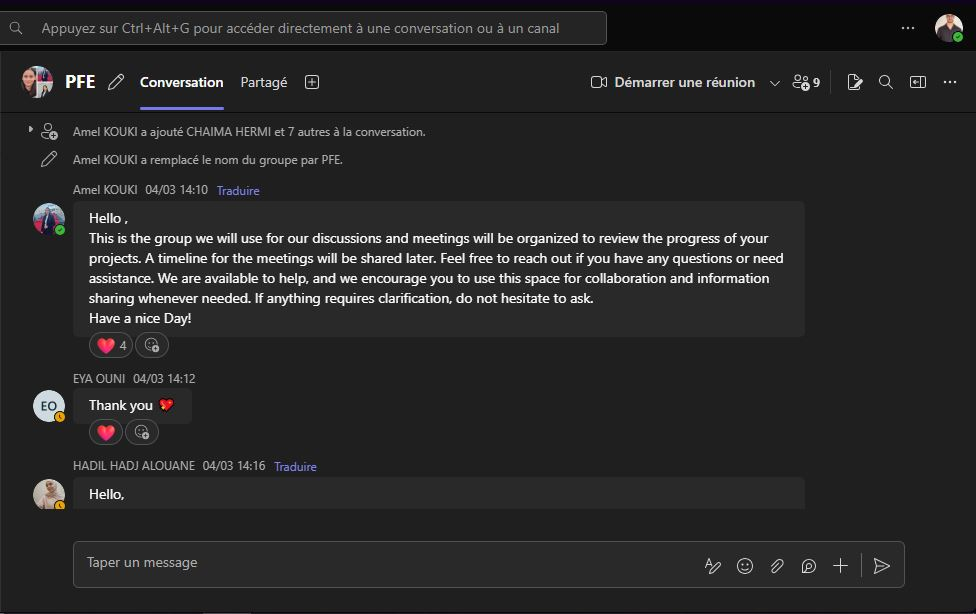
\includegraphics[width=0.85\textwidth]{images/teams.png}
  \caption{Interface de Microsoft Teams utilisée pour la communication et la collaboration.}
  \label{fig:teams}
\end{figure}

% ---------------------------------------------------------------
\section{Diagramme de Gantt}

Un diagramme de Gantt est un outil de planification visuel qui représente le calendrier d'un projet sous forme de barres horizontales. Chaque barre correspond à une tâche ou à un sprint : sa position sur l'axe du temps indique la date de début, sa longueur traduit la durée, et son extrémité droite marque la date de fin prévue. Ce type de diagramme permet d'avoir une vue d'ensemble claire et immédiate de l'enchaînement des activités et de l'état d'avancement du projet.

La figure~\ref{fig:gantt} présente le diagramme de Gantt de notre projet, qui retrace l'enchaînement des huit sprints Agile Scrum, depuis la mise en place initiale jusqu'à la finalisation et au déploiement de la plateforme.

%% Gantt — real sprint dates from git history (Mar 23 – Jul 31 2026 = 19 weeks)
\begin{figure}[H]
\centering
\begin{tikzpicture}[x=0.62cm, y=0.62cm]
  \def\nw{19}
  \def\nr{8}
  \fill[blue!6]  (0,0) rectangle (1.29,\nr);
  \fill[white]   (1.29,0) rectangle (5.57,\nr);
  \fill[blue!6]  (5.57,0) rectangle (10.0,\nr);
  \fill[white]   (10.0,0) rectangle (14.29,\nr);
  \fill[blue!6]  (14.29,0) rectangle (18.57,\nr);
  \foreach \x in {0,1,...,19} { \draw[gray!18] (\x,0) -- (\x,\nr); }
  \fill[blue!82!black] (0,\nr+0.75) rectangle (18.57,\nr+1.55);
  \node[text=white, font=\small\bfseries, anchor=center] at (9.285,\nr+1.15)
    {AI Intelligent Recruiter \textemdash{} Planning du projet (mars\textendash{}juillet 2026)};
  \fill[blue!55!black] (0,\nr) rectangle (18.57,\nr+0.75);
  \foreach \a/\b/\m in {0/1.29/Mars,1.29/5.57/Avril,5.57/10.0/Mai,10.0/14.29/Juin,14.29/18.57/Juillet}{
    \draw[white!50, thin] (\a,\nr) -- (\a,\nr+0.75);
    \node[text=white, font=\footnotesize\bfseries, anchor=center] at ({(\a+\b)/2},\nr+0.375) {\m};
  }
  \draw[white!50, thin] (18.57,\nr) -- (18.57,\nr+0.75);
  \foreach \a in {1.29,5.57,10.0,14.29}{ \draw[gray!40] (\a,0) -- (\a,\nr); }
  \draw[gray!60] (0,0) rectangle (18.57,\nr+1.55);
  \draw[red!60!black, dashed, line width=0.7pt] (10.43,0) -- (10.43,\nr);
  \node[font=\tiny, text=red!60!black, rotate=90, anchor=south] at (10.43,0.1) {Aujourd'hui};
  \foreach \i/\lab/\s/\e/\col in {
    0/{Sprint 0 : Mise en place \& Avatar 3D}/0/0.29/blue!65!black,
    1/{Sprint 1 : Moteur d'entretien agentique}/0.29/1.29/blue!65!black,
    2/{Sprint 2 : Exercices de code \& Docker}/1.29/3.0/blue!65!black,
    3/{Sprint 3 : Détection de fraude}/3.0/5.14/blue!65!black,
    4/{Sprint 4 : Profils \& Multimodal}/5.14/6.0/blue!65!black,
    5/{Sprint 5 : Intégration \& Quiz}/6.0/8.43/blue!65!black,
    6/{Sprint 6 : Consolidation \& Tests}/8.43/10.29/blue!65!black,
    7/{Sprint 7 : Finalisation \& Déploiement}/10.29/18.57/gray!40
  }{
    \pgfmathsetmacro{\yy}{\nr - 0.5 - \i}
    \node[anchor=east, font=\scriptsize] at (-0.2,\yy) {\lab};
    \fill[\col, draw=black!25, thin, rounded corners=1pt] (\s,\yy-0.30) rectangle (\e,\yy+0.30);
  }
\end{tikzpicture}
\caption{Diagramme de Gantt du projet : enchaînement des sprints Agile Scrum (mars--juillet~2026).}
\label{fig:gantt}
\end{figure}

\section{Conclusion}

Ce chapitre a permis de poser le cadre général du projet. Nous avons commencé par présenter l'entreprise d'accueil et ses domaines d'activité. Nous avons ensuite exposé la problématique, analysé les solutions existantes et présenté notre propre solution. Enfin, nous avons décrit la méthodologie adoptée, le découpage en sprints et le planning du projet.

Le chapitre suivant se concentrera sur l'analyse des besoins et la conception de la solution, en présentant les cas d'utilisation, l'architecture générale et les choix technologiques retenus.
     % Ch1 (1/2) : cadrage général du projet
    \chapter[Chapitre 2 : État de l'art et choix technologiques]{Chapitre 2 : État de l'art\\et choix technologiques}
\begin{spacing}{1.2}
\minitoc
\thispagestyle{MyStyle}
\end{spacing}
\clearpage

\section{Introduction}

Ce chapitre dresse un panorama des travaux académiques et des solutions industrielles en matière de recrutement assisté par l'IA, identifie les domaines de recherche qui fondent la conception de notre plateforme, et présente les technologies et \textit{frameworks} retenus pour chaque service. L'objectif est de justifier les choix techniques effectués et de situer le projet par rapport à l'état de l'art.

\section{État de l'art}

Le recrutement assisté par l'intelligence artificielle n'est pas un domaine nouveau, mais il a considérablement évolué ces dernières années avec l'avènement des grands modèles de langage et de l'analyse multimodale. Cette section fait le point sur les travaux et les outils existants dans les quatre domaines qui touchent directement notre plateforme : l'IA appliquée au recrutement, les modèles de langage et les \textit{workflows} agentiques, le traitement de la parole, et la vision par ordinateur. Pour chaque domaine, nous situons les approches courantes et nous indiquons le positionnement retenu dans le projet.

\subsection{L'intelligence artificielle dans le recrutement}

\subsubsection{Analyse automatique des CV et matching candidat-poste}

Les premiers systèmes de présélection automatique, les \textit{ATS} (\textit{Applicant Tracking Systems}), reposaient sur la recherche de mots-clés : le CV était comparé à une liste de termes attendus pour le poste. Ces outils ont réduit le travail manuel, mais au prix d'une grande rigidité — un candidat compétent qui n'employait pas exactement le vocabulaire de l'offre se trouvait écarté sans que personne ne le remarque.

L'arrivée des représentations vectorielles de mots, telles que Word2Vec puis GloVe, a permis de mesurer une proximité sémantique entre deux textes et de dépasser en partie ce problème de vocabulaire. Plus récemment, des modèles à base de \textit{transformers} tels que BERT ont été spécialisés pour la mise en correspondance entre un CV et une description de poste, en tenant compte du contexte des deux côtés. Notre plateforme s'inscrit dans cette lignée : le \textit{matching} ne se fait pas sur des mots-clés bruts, mais sur des \textit{embeddings} produits par des modèles de type Sentence-Transformers, indexés avec FAISS pour permettre une recherche rapide de proximité sémantique.

Une autre approche s'appuie sur les graphes de connaissances. Des plateformes comme Eightfold.ai relient compétences, intitulés de poste et secteurs d'activité pour déduire des qualifications implicites : un candidat qui mentionne « PyTorch » possède vraisemblablement des bases en \textit{deep learning}, même si l'expression n'apparaît pas explicitement dans son CV.

Le biais algorithmique reste un point sensible : un modèle entraîné sur des données de recrutement historiques risque de reproduire les biais de genre ou d'origine présents dans ces données. Notre plateforme limite ce risque en évaluant les candidats par rapport à une grille de critères dérivée de l'offre elle-même, et non d'historiques d'embauche antérieurs.

\subsubsection{IA conversationnelle pour l'entretien automatisé}

Les premiers systèmes d'entretien automatisé utilisaient des \textit{chatbots} à script, incapables de réagir à une réponse inattendue. Les grands modèles de langage ont changé la donne : il est désormais possible de mener un échange ouvert et adaptatif, d'ajuster la difficulté des questions, de relancer sur une réponse incomplète et de maintenir une conversation cohérente sur plusieurs tours.

Des plateformes commerciales comme HireVue ou Interviewer.ai font passer des entretiens vidéo en différé et notent les candidats à partir d'indices textuels et audio-visuels. Ces systèmes diffusent toutefois des questions préenregistrées et ne dialoguent pas en temps réel. C'est précisément là que se situe l'apport de notre solution, qui conduit un entretien synchrone, en direct, où l'agent réagit aux réponses du candidat.

Les architectures dites agentiques vont plus loin en découpant l'entretien en plusieurs phases coordonnées par une machine à états. Notre plateforme suit ce principe : une machine à états développée sur mesure pilote la progression, depuis la phase RH comportementale menée par l'agent conversationnel jusqu'à la phase technique, où les questions sont sélectionnées par un moteur adaptatif de type IRT/CAT.

\subsubsection{Évaluation multimodale du candidat}

Au-delà du texte, plusieurs travaux étudient les signaux audio et vidéo comme indicateurs de la qualité de communication d'un candidat. Des campagnes d'évaluation telles qu'AVEC ont montré que certaines caractéristiques paralinguistiques — débit de parole, hésitations, variations de hauteur de voix — et les unités d'action faciales sont corrélées, faiblement mais de façon constante, avec les notes attribuées par des recruteurs humains.

Les approches récentes combinent transcription, indices audio et \textit{embeddings} d'images vidéo pour produire un score global du candidat. Notre plateforme intègre ces signaux multimodaux à travers l'analyse de sentiment vocal et l'analyse des expressions faciales, en les traitant comme des indices complémentaires plutôt que comme la base de la décision finale, qui reste sous contrôle humain.

\subsubsection{Surveillance automatisée et contrôle d'intégrité}

Avec le passage au recrutement à distance, l'intégrité des évaluations en ligne est devenue un enjeu à la fois technique et éthique. Les solutions de surveillance se rangent en trois catégories : la \textbf{vérification d'identité}, qui confirme que la personne évaluée est bien le candidat attendu ; le \textbf{suivi de l'attention}, qui repère les déviations du regard, les changements de posture et de fenêtre ; et le \textbf{contrôle de l'environnement}, qui détecte des ressources non autorisées.

Des plateformes telles que Proctorio combinent flux caméra, verrouillage du navigateur et analyse de frappe. Les recherches ont toutefois signalé un taux de faux positifs préoccupant, en particulier lorsque la détection de visage perd en précision selon la couleur de peau. Notre plateforme répond à ce risque en croisant plusieurs signaux de détection — changement de fenêtre, détection d'objets par vision par ordinateur, vérification d'identité faciale — plutôt qu'en s'appuyant sur un seul indicateur. Aucune violation ne déclenche une disqualification automatique : toutes sont remontées au recruteur sous forme d'un rapport horodaté, qui tranche.

\subsection{Grands modèles de langage et \textit{workflows} agentiques}

\subsubsection{Modèles de langage à base de \textit{transformers}}

L'architecture \textit{transformer}, introduite par Vaswani \textit{et al.} en 2017, a remplacé les réseaux récurrents par un mécanisme d'auto-attention qui calcule en parallèle les relations entre tous les jetons d'une séquence. Ce choix a rendu possible l'entraînement sur des corpus bien plus volumineux qu'auparavant et a donné naissance au paradigme des modèles de langage pré-entraînés.

BERT a montré qu'un modèle pré-entraîné sur la prédiction de mots masqués pouvait ensuite être spécialisé sur des tâches précises avec très peu de données annotées supplémentaires. La famille GPT a exploré la voie autorégressive, en augmentant la taille de modèles décodeurs jusqu'à des centaines de milliards de paramètres et en faisant apparaître des capacités d'apprentissage à partir de quelques exemples seulement.

Pour notre plateforme, le moteur de dialogue repose sur le modèle \texttt{openai/gpt-oss-120b} servi via Groq, un modèle de type \textit{mixture-of-experts} de 117 milliards de paramètres. Sa capacité à suivre des instructions, son temps de réponse réduit et sa prise en charge des sorties structurées en JSON en font un choix adapté pour orchestrer un entretien à plusieurs tours et produire des grilles d'évaluation directement exploitables par le reste du système.

\subsubsection{\textit{Prompt engineering} et \textit{instruction tuning}}

Le \textit{prompt engineering} consiste à composer le contexte textuel fourni au modèle pour obtenir le comportement voulu, sans modifier ses poids. Plusieurs techniques sont utilisées dans notre plateforme :

\begin{itemize}
  \item \textbf{\textit{System prompts} :} un message prioritaire placé en tête de chaque conversation, qui fixe le rôle du modèle, ses contraintes et le format de sortie attendu. C'est par ce biais qu'est définie la personnalité de l'agent RH « Nour ».
  \item \textbf{Exemples \textit{few-shot} :} quelques paires entrée-sortie insérées dans le prompt pour orienter le style des réponses.
  \item \textbf{\textit{Chain-of-thought} :} le modèle est invité à produire un raisonnement explicite avant sa réponse finale, ce qui améliore la précision sur les tâches d'évaluation complexes.
  \item \textbf{Sortie structurée :} le modèle est contraint à répondre en JSON, ce qui permet aux étapes suivantes du système de consommer sa réponse de façon programmatique, sans analyse de chaîne de caractères fragile.
\end{itemize}

L'\textit{instruction tuning} — un réglage supervisé sur un jeu de paires instruction-réponse, suivi d'un apprentissage par renforcement à partir de retours humains (RLHF) — aligne le modèle de base sur les préférences humaines. C'est ce procédé qui produit les variantes optimisées pour le dialogue employées dans notre solution.

\subsubsection{\textit{Frameworks} agentiques et machines à états}

Au sens des LLM, un agent est un système qui utilise un modèle de langage comme moteur de raisonnement pour décider des actions à mener, les exécuter via des appels d'outils ou d'API, puis recommencer jusqu'à atteindre un objectif. Le paradigme ReAct (\textit{Reason + Act}) formalise cette boucle : le modèle alterne entre produire une réflexion, déclencher une action, observer le résultat, puis recommencer.

Des bibliothèques telles que LangChain et LangGraph proposent des briques réutilisables pour construire de tels agents : gabarits de \textit{prompts}, parseurs de sortie, et graphes d'exécution où les nœuds représentent les étapes de l'agent et les arêtes les transitions conditionnelles. Plutôt que de dépendre d'un de ces \textit{frameworks}, notre plateforme implémente sa propre machine à états, légère et entièrement maîtrisée, mieux adaptée aux contraintes de latence d'un entretien en direct.

Notre solution repose ainsi sur un agent conversationnel unique, « Nour », dont le comportement est piloté par cette machine à états plutôt que par une coordination entre plusieurs modèles distincts. Son fonctionnement s'articule autour de trois mécanismes :

\begin{itemize}
  \item deux \textbf{phases d'entretien} — une phase RH comportementale puis une phase technique — chacune dotée de son propre \textit{prompt} système ;
  \item une \textbf{sélection adaptative} des questions techniques fondée sur la théorie de réponse à l'item (IRT) ;
  \item des \textbf{modes de comportement} qui s'ajustent au niveau de stress détecté chez le candidat (normal, chaleureux, rassurant), afin de préserver son confort sans changer d'interlocuteur.
\end{itemize}

Ce choix d'une implémentation sur mesure maintient un contrôle explicite du flux et des contextes courts, tout en évitant la complexité d'un \textit{framework} agentique externe.

\subsection{Traitement de la parole}

\subsubsection{Reconnaissance automatique de la parole}

La reconnaissance automatique de la parole (ASR) transforme un signal audio brut en transcription textuelle. Les systèmes classiques associaient des modèles de Markov cachés (HMM) pour la modélisation temporelle à des mélanges de gaussiennes (GMM) pour la modélisation acoustique, et nécessitaient un lexique de prononciation et un modèle de langage distincts.

L'apprentissage profond a fait basculer ce domaine vers des modèles de bout en bout, qui apprennent directement la correspondance entre l'audio et le texte. La fonction de coût CTC (\textit{Connectionist Temporal Classification}) a permis un entraînement séquence à séquence sans alignement explicite, et les architectures encodeur-décodeur à attention comme LAS (\textit{Listen, Attend and Spell}) ont encore amélioré la précision. Le modèle wav2vec 2.0 a montré qu'un pré-entraînement auto-supervisé sur de l'audio brut pouvait atteindre des taux d'erreur compétitifs avec seulement quelques heures de données annotées.

Whisper, développé par OpenAI, est un modèle entraîné de façon faiblement supervisée sur des centaines de milliers d'heures d'audio multilingue. Son architecture encodeur-décodeur traite des spectrogrammes log-mel et atteint une précision proche de celle d'un humain en anglais, tout en restant performant sur de nombreuses langues. Notre plateforme utilise Faster-Whisper, une réimplémentation optimisée de Whisper qui réduit fortement le temps de transcription et la consommation mémoire — ce qui est indispensable pour transcrire les réponses du candidat au fil de l'entretien en temps réel.

\subsubsection{Synthèse vocale neuronale}

La synthèse vocale (TTS, \textit{Text-To-Speech}) transforme un texte écrit en parole. Les premiers systèmes reposaient sur la sélection d'unités (assemblage de segments de phonèmes préenregistrés) ou sur la synthèse par formants, et produisaient une voix intelligible mais artificielle.

WaveNet, un modèle génératif travaillant directement sur la forme d'onde au moyen de convolutions causales dilatées, a montré pour la première fois qu'une voix synthétique pouvait être difficile à distinguer d'une voix humaine. Les systèmes suivants, comme Tacotron 2 ou FastSpeech, ont séparé la prédiction du spectrogramme de la génération de la forme d'onde, ce qui a accéléré l'inférence. Les approches récentes (VITS, StyleTTS 2) savent moduler la prosodie et le débit, et reproduire une voix à partir d'un court extrait.

Pour la voix de l'agent conversationnel, notre plateforme s'appuie sur EdgeTTS, qui donne accès aux voix neuronales de Microsoft sans coût d'API. Ce choix s'inscrit dans la contrainte du projet de privilégier des outils gratuits ou exécutables localement. EdgeTTS fonctionne en \textit{streaming} : il commence à renvoyer des fragments audio avant la fin de la synthèse, ce qui limite le délai perçu et contribue à la fluidité de l'échange pendant l'entretien.

\subsubsection{ASR en contexte multilingue}

L'entretien se déroule principalement en français et en anglais, deux langues pour lesquelles Whisper offre une précision élevée sans adaptation particulière. Le choix de Faster-Whisper repose en grande partie sur cette couverture multilingue : un même modèle gère les deux langues d'entretien sans qu'il soit nécessaire de basculer entre plusieurs systèmes ASR.

Le dialecte tunisien (darija) constitue toutefois un cas difficile : il mêle l'arabe classique à des emprunts au français, à l'italien et au berbère, et n'a pas de forme écrite normalisée. Les systèmes entraînés sur l'arabe standard moderne y sont peu performants. Plusieurs pistes existent pour ces langues peu dotées — apprentissage par transfert, modèles multilingues partageant un même espace acoustique, augmentation de données par synthèse vocale — et leur intégration figure parmi les perspectives d'évolution de la plateforme.

\subsection{Vision par ordinateur pour le contrôle d'intégrité}

\subsubsection{Détection et suivi de visage}

La détection de visage consiste à localiser les visages humains dans une image ou une trame vidéo. L'algorithme de Viola-Jones (2001) a introduit le premier détecteur temps réel fondé sur des caractéristiques de type Haar et un classificateur en cascade. Les réseaux de neurones convolutifs profonds ont ensuite dominé les \textit{benchmarks} de détection de visage : MTCNN (\textit{Multi-task Cascaded Convolutional Networks}) et RetinaFace atteignent un rappel élevé même en cas d'occlusion, de variation d'éclairage ou de pose extrême.

Pour la réidentification d'identité, FaceNet a introduit une fonction de coût par triplets qui projette chaque image de visage dans un espace d'embeddings compact de 128 ou 512 dimensions, de sorte que la distance entre les \textit{embeddings} d'une même personne est minimisée et celle entre personnes différentes est maximisée. Cet espace permet une vérification d'identité en un seul exemple (\textit{one-shot}) sans réentraîner le modèle pour chaque nouvelle identité.

Google MediaPipe BlazeFace est un détecteur de visage léger et optimisé pour les appareils mobiles : il restitue six points-clés faciaux en plus de la boîte englobante, et tourne à plus de 200 images par seconde sur un GPU mobile. Ces caractéristiques en font un choix adapté au traitement trame par trame à faible latence requis par le module de détection de fraude de notre plateforme.

\subsubsection{Estimation du regard et suivi oculaire}

L'estimation du regard prédit l'endroit où une personne dirige son attention, soit comme un vecteur de direction 3D, soit comme un point d'intérêt 2D sur un écran. Les méthodes basées sur l'apparence régressent le regard à partir d'une image du visage entier ou d'un recadrage des yeux, à l'aide de CNN entraînés sur des jeux de données de regard tels que MPIIGaze ou GazeCapture.

L'EAR (\textit{Eye Aspect Ratio}) est une heuristique légère dérivée de six points de repère faciaux autour de chaque œil : elle quantifie le degré d'ouverture des yeux et est utilisée pour la détection des clignements et de la somnolence. Notre plateforme combine l'analyse par EAR avec le maillage facial 3D à 468 points de MediaPipe pour déterminer à la fois le taux de clignement et la direction du regard, et signaler tout regard hors écran prolongé comme une violation potentielle d'intégrité.

\subsubsection{Détection d'objets en environnement contrôlé}

La détection d'objets identifie et localise toutes les instances d'un ensemble de classes cibles dans une image. Les détecteurs à deux étapes (R-CNN, Faster R-CNN) génèrent d'abord des propositions de régions, puis classifient chaque région ; ils offrent une haute précision mais sont coûteux en calcul pour les applications temps réel.

Les détecteurs à une étape, comme la famille YOLO (\textit{You Only Look Once}), prédisent les probabilités de classe et les boîtes englobantes en une seule passe, ce qui permet une inférence en temps réel. YOLOv8 (Ultralytics) atteint des performances état de l'art sur le \textit{benchmark} COCO à des vitesses d'inférence supérieures à 100 images par seconde sur des GPU modernes. Il repose sur un \textit{backbone} CSPDarknet, un \textit{neck} PANet pour l'agrégation de caractéristiques multi-échelle et une tête de détection sans ancres (\textit{anchor-free}). Notre plateforme déploie la variante YOLOv8n (nano) pour identifier les objets interdits — téléphone mobile, écran secondaire, notes écrites, personne supplémentaire — dans le flux de la webcam du candidat pendant l'entretien.

\section{Technologies et \textit{frameworks} retenus}

Cette section décrit les technologies retenues pour la réalisation de notre plateforme. Pour chacune, nous précisons son rôle dans le système et la raison du choix.

% ── 2.3.1 ────────────────────────────────────────────────────────────────────
\subsection{\textit{Back-end} et couche API}

\subsubsection{FastAPI}

FastAPI (Python) porte les services liés à l'IA : le moteur d'entretien, l'analyse multimodale et la détection de fraude. Il expose des points d'accès WebSocket pour la communication bidirectionnelle en temps réel pendant l'entretien, servis par le \textit{runtime} ASGI Uvicorn. La documentation OpenAPI générée automatiquement, la validation des requêtes via Pydantic et la prise en charge native de \texttt{async}/\texttt{await} en font un choix adapté pour des services sensibles à la latence et fortement liés aux entrées-sorties, comme le traitement audio en flux.

\subsubsection{Node.js et Express}

Le service métier principal — gestion des utilisateurs, des offres d'emploi, des candidatures et des entretiens — est développé en Node.js avec le \textit{framework} Express. L'accès à la base de données passe par Mongoose, qui fournit une couche de modélisation au-dessus de MongoDB et permet de définir des schémas, des validations et des relations entre documents. Ce service expose l'API REST consommée par le \textit{front-end} React.

\subsubsection{MongoDB}

MongoDB est la base de données principale de la plateforme. Le projet utilise une base unique, \texttt{ai\_recruiter}, qui regroupe les entités candidats, recruteurs, offres, étapes de recrutement, entretiens, paires question-réponse et rapports de violation. Le choix d'une base NoSQL orientée documents se justifie par la nature des données manipulées : des objets imbriqués et de structure variable (transcriptions, résultats d'analyse, sessions d'entretien) qui s'expriment mal dans un schéma relationnel rigide. Cette base a fait l'objet d'une consolidation : trois bases distinctes ont été fusionnées en une seule pour simplifier l'accès aux données et les requêtes inter-collections.

\subsubsection{Redis}

Redis assure le stockage en mémoire de l'état de session du moteur d'entretien. Le contexte de l'entretien — question en cours, historique d'évaluation, sujets déjà abordés — y est conservé, ce qui lui permet de survivre à une coupure passagère de la connexion WebSocket sans obliger le client à retransmettre l'ensemble de l'état. Sa rapidité d'accès est adaptée à un usage où la latence est critique.

\subsubsection{Stockage local structuré}

Les fichiers volumineux — CV des candidats et enregistrements vidéo des entretiens — sont conservés sur le système de fichiers local du serveur, organisé en deux répertoires distincts : \texttt{uploads/} pour les CV et \texttt{recordings/} pour les vidéos. L'accès s'effectue via une route dédiée paramétrée par un identifiant de \texttt{bucket}, ce qui maintient une abstraction légère entre le code applicatif et l'emplacement physique des fichiers, tout en laissant la porte ouverte à une migration vers un stockage objet distribué.

% ── 2.3.2 ────────────────────────────────────────────────────────────────────
\subsection{Pile IA et modèles de langage}

\subsubsection{Groq — moteur d'inférence LLM}

Le moteur de dialogue de la plateforme repose sur le modèle \texttt{openai/gpt-oss-120b}, un modèle \textit{mixture-of-experts} de 117 milliards de paramètres, servi via l'API Groq. Groq exécute les modèles sur des puces LPU (\textit{Language Processing Unit}) spécialisées qui atteignent des débits de sortie nettement supérieurs à ceux des GPU classiques, ce qui réduit la latence perçue pendant l'entretien. Ce modèle assure la génération dynamique des questions, l'évaluation des réponses du candidat et l'orchestration du flux d'entretien ; sa prise en charge native des sorties structurées en JSON permet aux nœuds agents aval de consommer ses résultats directement.

\subsubsection{Moteur d'orchestration de l'entretien}

L'enchaînement de l'entretien n'est pas délégué à un \textit{framework} agentique externe, mais à une machine à états développée sur mesure en Python. Une structure \texttt{InterviewState} transporte l'ensemble du contexte de la session — phase courante, historique des évaluations, métadonnées de la dernière question — tandis qu'une énumération de phases distingue la phase RH comportementale de la phase technique, chacune associée à son propre \textit{prompt} système. À chaque tour, le moteur interroge le LLM (via Groq) pour générer la question suivante ou évaluer la réponse du candidat, sélectionne les questions techniques au moyen du moteur IRT, et ajuste le mode de comportement de l'agent selon le stress détecté. Ce contrôle explicite du flux, sans dépendance externe, facilite le débogage et garantit des temps de réponse compatibles avec un entretien en direct.

\subsubsection{EdgeTTS et ElevenLabs — synthèse vocale}

La synthèse vocale de l'agent repose sur deux fournisseurs. EdgeTTS, qui donne accès aux voix neuronales de Microsoft sans clé ni coût d'API, constitue le fournisseur par défaut : il fonctionne en \textit{streaming} et garantit le fonctionnement de la plateforme dans tous les environnements, sans configuration. ElevenLabs est proposé comme option premium, activée uniquement lorsqu'une clé API est explicitement configurée ; son API de \textit{streaming} émet les premiers fragments audio avant la fin de la synthèse, pour une latence au premier octet réduite. Ce choix s'inscrit dans la contrainte du projet de privilégier des outils gratuits ou exécutables localement, tout en laissant la possibilité d'une voix de meilleure qualité.

\subsubsection{Faster-Whisper — reconnaissance automatique de la parole}

Faster-Whisper est une réimplémentation optimisée du modèle Whisper d'OpenAI, utilisant le moteur CTranslate2 pour réduire la consommation mémoire et accélérer la transcription. Il est déployé localement dans le \textit{speech stack} et transcrit les réponses audio du candidat en temps réel. Le fournisseur ASR peut être sélectionné dynamiquement selon la langue configurée pour la session.

% ── 2.3.3 ────────────────────────────────────────────────────────────────────
\subsection{Vision par ordinateur et apprentissage automatique}

\subsubsection{OpenCV}

OpenCV 4.x est utilisé par le module de détection de fraude pour le décodage des trames, le prétraitement des images et les transformations géométriques appliquées aux flux webcam encodés en base64. Son noyau C++ accessible via des liaisons Python gère efficacement les opérations de traitement d'images à haute cadence, trame par trame.

\subsubsection{MediaPipe}

Google MediaPipe fournit la détection de maillage facial en temps réel, restituant 468 points de repère faciaux 3D par trame. Le module de surveillance utilise cette solution pour calculer l'\textit{Eye Aspect Ratio} (EAR) pour la détection des clignements et pour estimer la pose de la tête ainsi que la direction du regard dans le cadre de la surveillance de l'attention.

\subsubsection{YOLOv8 — Ultralytics}

YOLOv8 (Ultralytics) effectue la détection d'objets en temps réel pour identifier les éléments interdits — téléphones mobiles, écrans secondaires, livres et notes — ainsi que les personnes supplémentaires présentes dans l'environnement du candidat. La variante nano (\texttt{YOLOv8n}) a été retenue afin d'équilibrer précision et latence sur des cibles de déploiement sans GPU.

\subsubsection{PyTorch}

PyTorch sert de \textit{runtime} d'apprentissage profond pour le détecteur YOLO et le module de vérification d'identité. Son graphe de calcul dynamique et son support CUDA natif facilitent le chargement des modèles et l'inférence en temps réel.

\subsubsection{InsightFace — vérification d'identité}

InsightFace, avec le pack de modèles \texttt{buffalo\_l}, calcule un \textit{embedding} de 512 dimensions pour chaque visage détecté. La distance cosinus entre l'\textit{embedding} de référence — calculé à partir de la photo de profil du candidat lors de l'inscription — et chaque \textit{embedding} détecté en cours d'entretien permet d'identifier les tentatives d'usurpation d'identité. Le modèle est téléchargé automatiquement au premier lancement.

% ── 2.3.4 ────────────────────────────────────────────────────────────────────
\subsection{\textit{Front-end} et technologies client}

\subsubsection{React 19 et Vite}

L'interface utilisateur est développée avec React 19, en utilisant Vite 6 comme outil de construction et de développement. Vite offre un démarrage quasi instantané du serveur de développement et un rechargement à chaud des modules (\textit{HMR}), ce qui accélère sensiblement le cycle de développement. React Router DOM assure la navigation côté client, et Socket.IO Client gère la connexion WebSocket temps réel avec le \textit{speech stack} et le moteur d'entretien.

\subsubsection{Three.js, React Three Fiber et Drei}

L'avatar 3D de l'agent conversationnel est rendu dans le navigateur à l'aide de Three.js, avec React Three Fiber comme couche d'intégration déclarative dans React, et Drei pour les composants utilitaires (caméra, éclairage, contrôles orbitaux). La synchronisation labiale (\textit{lip-sync}) est assurée en associant les phonèmes du flux audio TTS aux \textit{morph targets} du maillage facial de l'avatar, pour un rendu naturel et synchronisé.

\subsubsection{Tailwind CSS et Radix UI}

Tailwind CSS fournit un système de styles utilitaires qui évite la prolifération de fichiers CSS séparés et maintient la cohérence visuelle de l'interface. Les composants d'interface accessibles — menus déroulants, boîtes de dialogue, onglets, infobulles — sont issus de la bibliothèque Radix UI, dont les primitives non stylisées sont entièrement compatibles avec les classes Tailwind.

% ── 2.3.5 ────────────────────────────────────────────────────────────────────
\subsection{Infrastructure et DevOps}

\subsubsection{Docker et Docker Compose}

Les services IA (moteur d'entretien, service d'analyse, service YOLO, service de vérification faciale) sont conteneurisés avec Docker. Docker Compose orchestre les dépendances entre services lors du déploiement local et en environnement de test : chaque service dispose de son propre \textit{Dockerfile}, et des variantes CPU et GPU sont prévues pour les services d'inférence lourde.

\subsubsection{WebSocket et Socket.IO}

La communication temps réel entre le \textit{front-end} et les services Python repose sur deux protocoles complémentaires. Socket.IO assure la signalisation entre le navigateur et le serveur Node.js (notifications, état de la salle d'entretien, mises à jour de score). Les connexions WebSocket natives, gérées par FastAPI/Uvicorn, transportent les flux audio et les réponses de l'agent pendant l'entretien, en minimisant la surcharge de protocole pour les données à haute fréquence.

\section{Conclusion}

Ce chapitre a dressé un panorama de l'état de l'art en matière de recrutement assisté par l'IA, de traitement automatique de la parole et de surveillance par vision par ordinateur, et a présenté les choix technologiques retenus pour chaque couche de notre plateforme. La littérature confirme que les entretiens agentiques pilotés par LLM, la synthèse vocale neuronale, la transcription multilingue par Whisper et la détection d'objets par YOLOv8 représentent l'état de l'art dans leurs domaines respectifs. La pile technologique retenue — Groq/LangGraph pour l'orchestration des agents, Faster-Whisper et ElevenLabs/EdgeTTS pour le traitement de la parole, InsightFace et MediaPipe pour la surveillance, et React/Three.js pour l'interface — équilibre productivité de développement, capacité IA et flexibilité opérationnelle. Le chapitre suivant détaille l'architecture du système et les décisions de conception qui intègrent ces technologies en une plateforme cohérente.

     % Ch1 (2/2) : analyse et conception
    % Chapitres 2 à 6 : un chapitre par sprint (réalisation et tests).
    % Anciens fichiers 07-Chapitre3 et 08-Chapitre4 conservés mais non inclus.
    \chapter[Sprint 1 : Socle applicatif et présélection]{Sprint 1 : Socle applicatif\\et présélection intelligente des candidats}
\begin{spacing}{1.2}
\minitoc%
\thispagestyle{MyStyle}
\end{spacing}
\clearpage

\providecommand{\screenshot}[2]{%
  \IfFileExists{../screenshoot/#1}{%
    \includegraphics[width=0.9\textwidth,height=12cm,keepaspectratio]{../screenshoot/#1}%
  }{%
    \fbox{\parbox[c][4.5cm][c]{0.9\textwidth}{\centering\itshape
      Capture d'écran à insérer~: #2\\[4pt]
      \normalfont\small(fichier attendu~: \texttt{screenshoot/#1})}}%
  }%
}

\section{Introduction}

Ce premier sprint pose les fondations de la plateforme NextHire. Il met en place l'environnement de développement, la structure du dépôt, le socle technique du back-end (API REST Node.js, authentification) et les briques de présélection des candidats~: analyse automatique des CV, recommandation d'offres et premiers écrans candidat et recruteur. À l'issue de ce sprint, un candidat peut s'inscrire, téléverser son CV et recevoir des offres recommandées, et un recruteur peut publier une offre.

\section{Objectifs du sprint}

L'objectif principal de ce sprint est défini comme suit~:

\begin{quote}
\itshape Établir les fondations techniques de la plateforme NextHire et son socle de présélection intelligente~: permettre à un candidat de s'inscrire, de téléverser son CV pour en extraire automatiquement un profil structuré et de recevoir des offres recommandées, et à un recruteur de publier une offre assortie d'un quiz de présélection.
\end{quote}

\subsection{Backlog du sprint}

Le tableau~\ref{tab:backlog-s1} présente le backlog de ce sprint~: les récits utilisateurs et tâches techniques sélectionnés depuis le \textit{product backlog} lors de la réunion de planification (\textit{sprint planning}). Comme pour le \textit{product backlog}, chaque élément est priorisé selon la méthode \textbf{MoSCoW} (\textbf{Must}, \textbf{Should}, \textbf{Could}) et estimé en \textit{story points} sur la suite de Fibonacci (1, 2, 3, 5, 8, 13), soit un engagement de 48~points pour ce sprint.

\begin{table}[H]
  \centering
  \footnotesize
  \renewcommand{\arraystretch}{1.3}
  \setlength{\tabcolsep}{5pt}
  \begin{tabularx}{\textwidth}{|>{\centering\arraybackslash}p{1.1cm}|>{\raggedright\arraybackslash}X|>{\centering\arraybackslash}p{1.7cm}|>{\centering\arraybackslash}p{0.9cm}|}
    \hline
    \rowcolor{blue!10}
    \textbf{ID} & \textbf{Récit utilisateur / tâche} & \textbf{Priorité} & \textbf{Est.} \\
    \hline
    T-01 & Initialiser le dépôt Git et la structure \textit{front-end} (React/Vite) et \textit{back-end} (Node.js/Express). & Must & 5 \\
    \hline
    S1 & En tant que candidat, je veux créer un compte et me connecter (JWT ou Google OAuth) afin d'accéder à la plateforme. & Must & 5 \\
    \hline
    S2 & En tant que candidat, je veux téléverser mon CV et obtenir automatiquement un profil structuré (extraction, OCR, analyse NLP). & Must & 8 \\
    \hline
    S3 & En tant que candidat, je veux consulter les offres d'emploi et soumettre une candidature. & Must & 3 \\
    \hline
    S4 & En tant que candidat, je veux recevoir des offres recommandées correspondant à mon profil. & Must & 5 \\
    \hline
    S5 & En tant que candidat, je veux relier mon compte LinkedIn afin d'enrichir mon profil. & Should & 3 \\
    \hline
    S6 & En tant que recruteur, je veux publier une offre d'emploi via l'assistant de création (\textit{Job Wizard}). & Must & 5 \\
    \hline
    S7 & En tant que candidat, je veux passer le quiz de présélection généré automatiquement pour ma candidature afin d'accéder à l'entretien. & Must & 5 \\
    \hline
    S8 & En tant que recruteur, je veux consulter le quiz de présélection de chaque candidature et le score obtenu par le candidat. & Must & 3 \\
    \hline
    S9 & En tant que candidat, je veux suivre le statut de ma candidature depuis mon tableau de bord afin de rester informé de son avancement. & Should & 3 \\
    \hline
    S10 & En tant que recruteur, je veux consulter la liste des candidatures et les profils détaillés afin d'étudier les candidats. & Must & 3 \\
    \hline
  \end{tabularx}
  \caption{Backlog du Sprint~1 : socle applicatif et présélection intelligente.}
  \label{tab:backlog-s1}
\end{table}

\section{Concept du socle de présélection}

Avant l'entretien proprement dit, NextHire filtre et qualifie les candidatures de façon \textit{intelligente}, sans se limiter à une recherche de mots-clés. Ce socle de présélection combine trois mécanismes complémentaires~: l'\textbf{analyse automatique du CV}, qui transforme un document hétérogène en profil structuré~; la \textbf{recommandation d'offres}, qui rapproche ce profil des postes ouverts par similarité sémantique et recouvrement de compétences~; et le \textbf{quiz de présélection}, qui vérifie objectivement les compétences déclarées avant l'accès à l'entretien.

L'ensemble s'appuie sur une base technique commune~: un \textit{front-end} React, un serveur Node.js jouant le rôle de point d'entrée unique, et une authentification centralisée qui oriente chaque utilisateur vers l'espace correspondant à son rôle (candidat, recruteur ou administrateur).

\section{Conception détaillée et architecture}

\subsection{Architecture du socle}

L'architecture micro-services et le pipeline de recommandation hybride ont été présentés en détail au chapitre~\ref{ch:sprint0} (Sprint~0). Ce sprint en concrétise le socle~: le serveur Node.js joue le rôle de point d'entrée unique (\textit{Backend For Frontend}), l'authentification est centralisée par jetons JWT, et la présélection des candidats repose sur deux micro-services Python indépendants, l'un dédié à l'analyse des CV, l'autre à la recommandation d'offres.

\subsection{Inscription, authentification et routage par rôle}

L'inscription crée un compte avec un rôle (candidat, recruteur ou administrateur)~; le mot de passe est haché par \texttt{bcrypt}. À la connexion, le serveur vérifie le mot de passe, signe un jeton JWT portant l'identité et le rôle, puis le client est routé vers l'espace correspondant (contrôle d'accès par rôle, RBAC). La figure~\ref{fig:seq-auth} illustre ce flux.

\begin{figure}[H]
  \centering
  \resizebox{0.85\textwidth}{!}{%
  \begin{tikzpicture}[
    font=\scriptsize, >={Stealth[length=2mm]},
    msg/.style={->, thin}, ret/.style={->, thin, dashed},
    lbl/.style={font=\tiny, fill=white, inner sep=1pt, midway, above},
    lifeline/.style={dashed, thin, gray!70},
    phdr/.style={draw, fill=blue!12, rounded corners=2pt, align=center,
                 font=\scriptsize\bfseries, minimum height=0.7cm, minimum width=2.8cm},
  ]
    \node[phdr] at ( 0,0) {Client\\(React)};
    \node[phdr] at ( 5,0) {Node BFF\\(:3001)};
    \node[phdr] at (10,0) {MongoDB};
    \foreach \x in {0,5,10}{ \draw[lifeline] (\x,-0.42) -- (\x,-8.0); }

    \draw[msg] ( 0,-0.85) -- node[lbl] {POST /api/auth/register \{email, rôle\}} (5,-0.85);
    \draw[->] (5,-1.35) -- ++(0.5,0) -- ++(0,-0.35) -- ++(-0.5,0);
    \node[font=\tiny, anchor=west] at (5.6,-1.52) {hacher le mot de passe (bcrypt)};
    \draw[msg] ( 5,-2.15) -- node[lbl] {insert User \{rôle\}} (10,-2.15);
    \draw[ret] (10,-2.75) -- node[lbl] {\{userId\}} (5,-2.75);
    \draw[ret] ( 5,-3.35) -- node[lbl] {201 Created} (0,-3.35);

    \draw[draw=gray!55, fill=gray!8, rounded corners=2pt, thin] (1.2,-3.75) rectangle (8.8,-4.2);
    \node[font=\tiny, anchor=west] at (1.3,-3.97) {Connexion ultérieure du candidat};

    \draw[msg] ( 0,-4.6) -- node[lbl] {POST /api/auth/login \{email, mot de passe\}} (5,-4.6);
    \draw[msg] ( 5,-5.2) -- node[lbl] {findOne(email)} (10,-5.2);
    \draw[ret] (10,-5.8) -- node[lbl] {\{user, hash\}} (5,-5.8);
    \draw[->] (5,-6.3) -- ++(0.5,0) -- ++(0,-0.35) -- ++(-0.5,0);
    \node[font=\tiny, anchor=west] at (5.6,-6.47) {vérifier bcrypt + signer le JWT \{id, rôle\}};
    \draw[ret] ( 5,-7.1) -- node[lbl] {200 OK \{token\}} (0,-7.1);
    \draw[->] (0,-7.6) -- ++(-0.5,0) -- ++(0,-0.0) ;
    \node[font=\tiny, anchor=west, text width=4.2cm] at (0.2,-7.75) {routage RBAC $\rightarrow$ espace candidat / recruteur / admin};
  \end{tikzpicture}}
  \caption{Diagramme de séquence : inscription, authentification et routage par rôle.}
  \label{fig:seq-auth}
\end{figure}

\subsection{Téléversement du CV, analyse et recommandation}

Le candidat téléverse son CV~; le serveur le confie à un micro-service d'analyse qui en extrait un profil structuré, puis sollicite le micro-service de recommandation pour proposer les offres les plus adaptées. La figure~\ref{fig:seq-cv-reco} détaille ce flux.

\begin{figure}[H]
  \centering
  \resizebox{\textwidth}{!}{%
  \begin{tikzpicture}[
    font=\scriptsize, >={Stealth[length=2mm]},
    msg/.style={->, thin}, ret/.style={->, thin, dashed},
    lbl/.style={font=\tiny, fill=white, inner sep=1pt, midway, above},
    lifeline/.style={dashed, thin, gray!70},
    phdr/.style={draw, fill=blue!12, rounded corners=2pt, align=center,
                 font=\scriptsize\bfseries, minimum height=0.7cm, minimum width=2.5cm},
  ]
    \node[phdr] at ( 0,0) {Candidat\\(React)};
    \node[phdr] at ( 4.5,0) {Node BFF\\(:3001)};
    \node[phdr] at ( 9,0) {Parseur CV\\(:5002)};
    \node[phdr] at (14,0) {Recommandation\\(:5001)};
    \node[phdr] at (18.5,0) {MongoDB};
    \foreach \x in {0,4.5,9,14,18.5}{ \draw[lifeline] (\x,-0.42) -- (\x,-8.6); }

    \draw[msg] ( 0,-0.85) -- node[lbl] {POST /api/users/cv (multipart)} (4.5,-0.85);
    \draw[->] (4.5,-1.35) -- ++(0.5,0) -- ++(0,-0.35) -- ++(-0.5,0);
    \node[font=\tiny, anchor=west] at (5.1,-1.52) {stocker le fichier (Multer)};
    \draw[msg] ( 4.5,-2.15) -- node[lbl] {POST /upload \{fichier\}} (9,-2.15);
    \draw[->] (9,-2.65) -- ++(0.5,0) -- ++(0,-0.35) -- ++(-0.5,0);
    \node[font=\tiny, anchor=west] at (9.6,-2.82) {extraction (pdfplumber / OCR) + NER};
    \draw[ret] ( 9,-3.45) -- node[lbl] {\{profil structuré\}} (4.5,-3.45);
    \draw[msg] ( 4.5,-4.05) -- node[lbl] {update User.profile} (18.5,-4.05);
    \draw[ret] ( 4.5,-4.65) -- node[lbl] {200 OK \{profil\}} (0,-4.65);

    \draw[draw=gray!55, fill=gray!8, rounded corners=2pt, thin] (1.5,-5.05) rectangle (12.5,-5.5);
    \node[font=\tiny, anchor=west] at (1.6,-5.27) {Recommandation d'offres pour le candidat};

    \draw[msg] ( 0,-5.9) -- node[lbl] {GET /recommendation/for-user} (4.5,-5.9);
    \draw[msg] ( 4.5,-6.5) -- node[lbl] {POST /recommend \{profil\}} (14,-6.5);
    \draw[->] (14,-7.0) -- ++(0.5,0) -- ++(0,-0.35) -- ++(-0.5,0);
    \node[font=\tiny, anchor=west] at (14.6,-7.17) {score hybride (FAISS + compétences)};
    \draw[ret] (14,-7.8) -- node[lbl] {\{offres classées\}} (4.5,-7.8);
    \draw[ret] ( 4.5,-8.4) -- node[lbl] {\{offres recommandées\}} (0,-8.4);
  \end{tikzpicture}}
  \caption{Diagramme de séquence : téléversement du CV, analyse et recommandation d'offres.}
  \label{fig:seq-cv-reco}
\end{figure}

\section{Réalisation et interfaces utilisateur}

\subsection{API REST du back-end}

Le backend Node.js (Express) expose une API REST organisée selon une convention de nommage
orientée ressources. L'ensemble des points de terminaison est regroupé sous le préfixe
\texttt{/api} et retourne des réponses JSON. Le serveur joue le rôle de point d'entrée unique
(\textit{Backend For Frontend}) : il monte une quinzaine de routeurs Express thématiques,
chacun responsable d'un domaine fonctionnel. Le tableau~\ref{tab:api-groups} récapitule les
principaux groupes de points de terminaison.

\begin{table}[H]
  \centering
  \footnotesize
  \renewcommand{\arraystretch}{1.3}
  \setlength{\tabcolsep}{5pt}
  \begin{tabularx}{\textwidth}{|>{\raggedright\arraybackslash}p{3.6cm}|>{\raggedright\arraybackslash}p{3.4cm}|>{\raggedright\arraybackslash}X|}
    \hline
    \rowcolor{blue!10}
    \textbf{Préfixe} & \textbf{Routeur} & \textbf{Rôle} \\
    \hline
    \texttt{/api/auth}, \texttt{/api/users} & \texttt{userRoute} & Connexion, inscription, OAuth Google, profils candidat et recruteur, enrôlement facial \\
    \hline
    \texttt{/api/jobs} & \texttt{jobRoute} & Gestion des offres d'emploi \\
    \hline
    \texttt{/api/wizard/jobs} & \texttt{jobWizardRoute} & Assistant de création d'offre (Job Wizard) \\
    \hline
    \texttt{/api/interviews} & \texttt{interviewRoute} & Cycle de vie de l'entretien, événements d'intégrité, rapports \\
    \hline
    \texttt{/api/call-rooms} & \texttt{callRoom} + \texttt{mediaRoute} & Sessions d'entretien IA, surveillance vision, enregistrements \\
    \hline
    \texttt{/api/job-rooms} & \texttt{jobInterviewRoom} & Salles d'entretien partageables, comparaison des candidats \\
    \hline
    \texttt{/quiz} & \texttt{quizRoute} & Quiz de présélection et modèles de quiz \\
    \hline
    \texttt{/api/messages} & \texttt{messages} & Messagerie temps réel recruteur / candidat \\
    \hline
    \texttt{/api/recommendations} & \texttt{recommendationRoute} & Recommandation d'offres basée sur le profil \\
    \hline
    \texttt{/api/recruiter/calendar}, \texttt{/api/internal/scheduling} & \texttt{recruiterCalendar}, \texttt{schedulingInternal} & Planification d'entretiens et intégration Google Calendar \\
    \hline
    \texttt{/api/linkedin} & \texttt{linkedinRoute} & Liaison et enrichissement du profil LinkedIn \\
    \hline
  \end{tabularx}
  \caption{Principaux groupes de points de terminaison REST du backend NextHire.}
  \label{tab:api-groups}
\end{table}

La validation des données entrantes est réalisée directement dans les gestionnaires de routes
et au niveau des schémas Mongoose, qui appliquent les contraintes de type, les champs requis,
les valeurs énumérées et l'unicité (par exemple l'adresse courriel). Plusieurs limiteurs de
débit (\texttt{express-rate-limit}), adossés en option à Redis, protègent les points de
terminaison sensibles tels que la génération de quiz par IA et la soumission des réponses.

\subsection{Authentification et autorisation}

L'authentification repose sur les jetons web JSON (JWT). Le déroulement est le suivant :

\begin{enumerate}
  \item Le client envoie une requête \texttt{POST /api/auth/login} avec son adresse courriel
        et son mot de passe.
  \item Le backend recherche l'utilisateur, vérifie le mot de passe haché avec
        \texttt{bcrypt}, puis génère un JWT signé contenant l'identifiant, l'adresse courriel
        et le rôle de l'utilisateur (\texttt{jwt.sign(\allowbreak\{id, email, role\}\allowbreak)}).
  \item Le client transmet ce JWT en tant que jeton \textit{Bearer} dans l'en-tête
        \texttt{Authorization} de toutes les requêtes suivantes.
  \item Le middleware \texttt{verifyToken} valide la signature et la date d'expiration du
        jeton avant de transmettre la requête ; toute requête non authentifiée reçoit une
        réponse \texttt{401}, de sorte que les gestionnaires métier ne traitent jamais de
        trafic anonyme.
  \item Le contrôle d'accès basé sur les rôles est assuré par le middleware
        \texttt{requireEnterprise} : les points de terminaison réservés au recruteur rejettent
        les requêtes au rôle candidat, avec un repli sur une vérification en base pour les
        jetons antérieurs ne portant pas encore le champ \texttt{role}.
\end{enumerate}

L'authentification via Google OAuth~2.0 est proposée comme méthode de connexion alternative.
Elle s'appuie sur la stratégie \texttt{passport-google-oauth20} : après autorisation de
l'utilisateur, le profil Google est récupéré via le \textit{callback}
\texttt{/auth/google/callback}, l'utilisateur est créé ou retrouvé en base, et un JWT
natif de la plateforme lui est délivré. Les jetons d'accès et de rafraîchissement Google sont
conservés pour permettre l'intégration ultérieure avec Google Calendar.

\subsection{Module d'extraction et d'analyse de CV}

Lorsqu'un candidat téléverse son CV, le fichier binaire (PDF ou image) est reçu par le
middleware \texttt{Multer} et stocké sur le système de fichiers local du serveur. L'analyse
est ensuite déléguée à un micro-service Python (Flask, port~5002) dédié, qui transforme un
document non structuré en un profil candidat exploitable par la plateforme.

\subsubsection{Extraction du texte (pipeline à deux niveaux)}

L'extraction du texte suit une stratégie en deux niveaux, choisie selon la nature du document~:

\begin{itemize}
  \item \textbf{Extraction native (PDF textuels).} La bibliothèque \texttt{pdfplumber} extrait
        le texte directement du PDF. Une reconstruction \textit{column-aware} a été développée
        pour traiter les CV sur deux colonnes~: un histogramme des positions horizontales des
        mots détecte l'espace inter-colonnes, puis le texte est recomposé colonne de gauche puis
        colonne de droite, afin d'éviter le mélange de lignes que produit l'ordre de lecture par
        défaut.
  \item \textbf{Reconnaissance optique (OCR) en repli.} Lorsque le texte natif est insuffisant
        (moins de 120~caractères ou de 20~mots) ou que le document est une image, le service
        rasterise chaque page avec \texttt{PyMuPDF} (facteur~2$\times$), puis applique
        \textbf{PaddleOCR} (modèle anglais, correction de l'orientation des lignes de texte)
        pour reconstruire le contenu. Le texte retenu est celui qui maximise la quantité
        d'information extraite.
\end{itemize}

Le texte obtenu est normalisé (suppression du bruit typographique, des artefacts
\texttt{(cid:n)} et des séparateurs) avant la phase d'analyse.

\subsubsection{Analyse et structuration du profil}

Le texte nettoyé est ensuite analysé par un pipeline de traitement du langage naturel combinant
la bibliothèque \texttt{spaCy} (modèle \texttt{en\_core\_web\_sm}) et un ensemble de règles et
d'expressions régulières bilingues (français/anglais). Ce pipeline extrait les champs
structurés du profil~: \texttt{name}, \texttt{email}, \texttt{phone}, \texttt{skills},
\texttt{languages}, \texttt{experience} (titre, entreprise, durée, description) et
\texttt{education}. Les compétences sont reconnues à partir d'un dictionnaire de référence
(\texttt{skills\_\allowbreak list.txt}), puis normalisées (par exemple \texttt{nodejs}~$\rightarrow$~%
\texttt{Node.js}) et filtrées par un validateur qui écarte les faux positifs (mots génériques,
fragments de phrases, encodages corrompus). Un \textbf{détecteur de domaine} classe enfin le
profil parmi dix familles métier (IA / \textit{Machine Learning}, \textit{data science},
développement logiciel, \textit{DevOps} / \textit{Cloud}, cybersécurité, finance, marketing,
ressources humaines, \textit{design} UX/UI et gestion de projet) par pondération des mots-clés rencontrés.

Pour écarter les documents qui ne sont pas des CV, un \textbf{classifieur binaire} valide le
résultat~: un modèle TF-IDF (n-grammes de 1 à 2) couplé à une régression logistique, entraîné
sur un jeu d'exemples étiquetés (CV contre factures, menus, relevés bancaires, etc.), produit
une probabilité d'appartenance à la classe «~CV~». Cette probabilité est combinée à des
heuristiques (présence de coordonnées, densité de mots-clés, présence de sections structurées)
pour accepter ou rejeter le document. Le profil validé est persisté dans le sous-document
\texttt{profile} de l'entité \texttt{User}, où il sert de contexte à l'agent d'entretien et au
moteur de recommandation décrit ci-après.

\subsection{Module de recommandation et de \textit{matching} d'offres}

Le \textit{matching} entre candidats et offres est assuré par un second micro-service Python
(Flask, port~5001) qui implémente une approche hybride combinant similarité sémantique et
recouvrement explicite des compétences.

\subsubsection{Représentation sémantique et indexation}

Chaque offre ouverte est convertie en un texte agrégé (titre, description, compétences,
langues) puis encodée en un vecteur dense de 384~dimensions par le modèle
\textbf{Sentence-Transformers} \texttt{all-MiniLM-L6-v2}. Si la bibliothèque n'est pas
disponible, le service bascule automatiquement sur un encodeur de repli
(\texttt{HashingVectorizer} de scikit-learn, 384~dimensions), ce qui garantit la continuité de
service. Les vecteurs sont normalisés et indexés dans un index \textbf{FAISS}
(\texttt{IndexFlatIP})~: le produit scalaire sur des vecteurs normalisés équivaut à une
similarité cosinus, ce qui permet une recherche des plus proches voisins efficace. L'index est
reconstruit périodiquement (toutes les heures, ou à la demande via un point d'accès dédié).

\subsubsection{Score hybride}

Le profil du candidat (résumé, compétences, langues, expériences) est encodé et normalisé de la
même manière, puis comparé à l'index FAISS pour obtenir un ensemble d'offres candidates avec
leur score sémantique. Le score final combine deux composantes~:
\[
  \text{score} = 0{,}25 \times \text{(similarité sémantique)} + 0{,}75 \times \text{(recouvrement pondéré des compétences)}.
\]
Le recouvrement des compétences est calculé après canonicalisation des intitulés (un
dictionnaire de synonymes ramène par exemple \texttt{js}, \texttt{reactjs} ou \texttt{node} à
leur forme canonique), puis pondéré~: chaque compétence porte un poids reflétant son importance
pour le poste (les technologies cœur comme React ou JavaScript pèsent davantage que des outils
secondaires). Une offre déjà candidatée par le candidat est exclue des résultats, et seules les
offres dont le score dépasse un seuil configurable (0{,}3 par défaut) sont retournées, classées
par pertinence décroissante. Chaque recommandation expose enfin le détail de son score
(part sémantique et part compétences), ce qui rend le \textit{matching} transparent pour le
candidat.

\subsection{Quiz de présélection et enrichissement LinkedIn}

En complément du \textit{matching}, le socle de présélection comprend un quiz technique de présélection. Dès qu'un candidat postule à une offre, un questionnaire personnalisé est généré automatiquement par l'IA (micro-service de génération de quiz) à partir des compétences attendues pour le poste et de celles du candidat, sans intervention du recruteur~; le candidat doit le réussir avant d'accéder à l'entretien, et les soumissions sont protégées par un limiteur de débit afin d'éviter les tentatives répétées. Par ailleurs, le candidat peut relier son compte LinkedIn à son profil~: un service d'enrichissement récupère ses données professionnelles publiques et complète automatiquement les compétences et expériences détectées dans le CV.

\subsection{Aperçu de l'interface utilisateur}

L'application cliente de NextHire est une application web monopage développée avec React~19
et empaquetée par Vite. Contrairement à une application de bureau, elle s'exécute
intégralement dans le navigateur et ne nécessite aucune installation. Le routage est assuré
par \texttt{react-router-dom}, qui distingue les espaces propres à chaque rôle : les écrans
candidat (profil, planification, salle d'entretien) et les écrans recruteur (espace
entreprise, salles d'entretien, comparaison des candidats), en plus d'un tableau de bord
d'administration.

La protection des routes et la gestion de session reposent sur un contexte React partagé,
\texttt{AuthContext}. À la connexion, le jeton JWT est conservé dans le \texttt{localStorage}
du navigateur, puis attaché à chaque appel au backend sous la forme d'un en-tête
\texttt{Authorization: Bearer <token>}. En cas de réponse signalant un jeton expiré ou
invalide, le contexte déconnecte l'utilisateur et le redirige vers la page de connexion. La
communication en temps réel (entretien, messagerie, alertes d'intégrité) s'appuie quant à
elle sur le client \texttt{socket.io-client}.

\subsection{Écrans candidat}

\subsubsection{Inscription et connexion}

L'accès à la plateforme commence par la page d'inscription et de connexion (routes \texttt{/register} et \texttt{/login}). Le candidat crée un compte avec son adresse courriel et un mot de passe, ou se connecte directement via \textbf{Google OAuth~2.0}. À l'authentification, le jeton JWT délivré par le serveur est conservé côté client et l'utilisateur est redirigé, selon son rôle, vers l'espace correspondant (figure~\ref{fig:login}).

\begin{figure}[H]
  \centering
  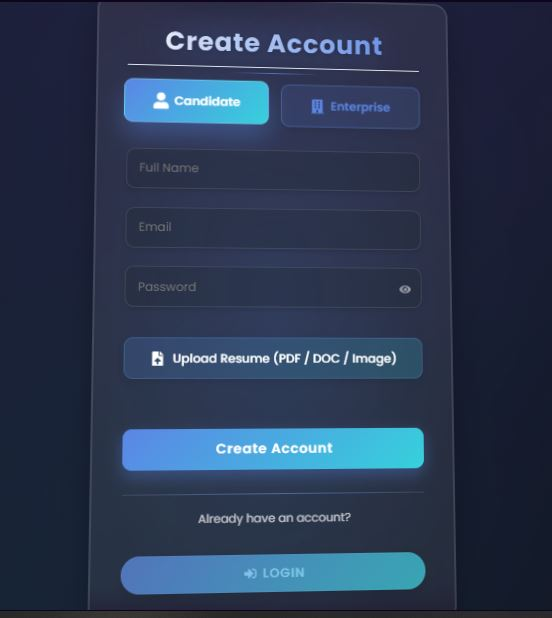
\includegraphics[width=0.48\textwidth,keepaspectratio]{../screenshoot/signup.JPG}\hfill
  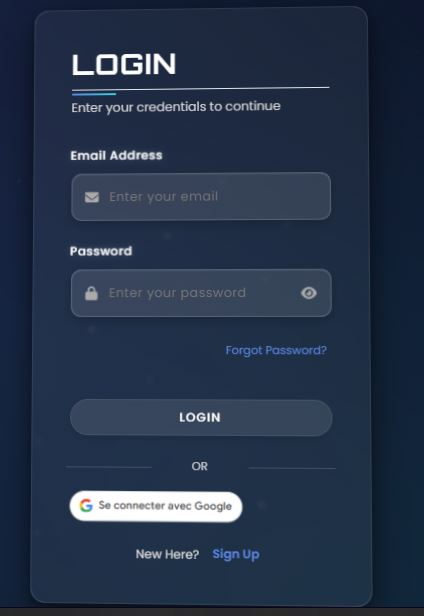
\includegraphics[width=0.48\textwidth,keepaspectratio]{../screenshoot/login.JPG}
  \caption{Écran d'inscription (à gauche) et de connexion (à droite) du candidat.}
  \label{fig:login}
\end{figure}

\subsubsection{Profil et tableau de bord candidat}

L'écran de profil candidat (route \texttt{/candidate/:id}) centralise les informations du
candidat : photo de profil vérifiée pour le contrôle d'identité, compétences, langues,
expériences et CV téléversé. Il présente également les candidatures soumises et les offres
recommandées par le moteur de recommandation. Un indicateur de complétude du profil incite
le candidat à compléter ses informations et à téléverser son CV, étape nécessaire avant de
postuler (figure~\ref{fig:candidate-profile}).

\begin{figure}[H]
  \centering
  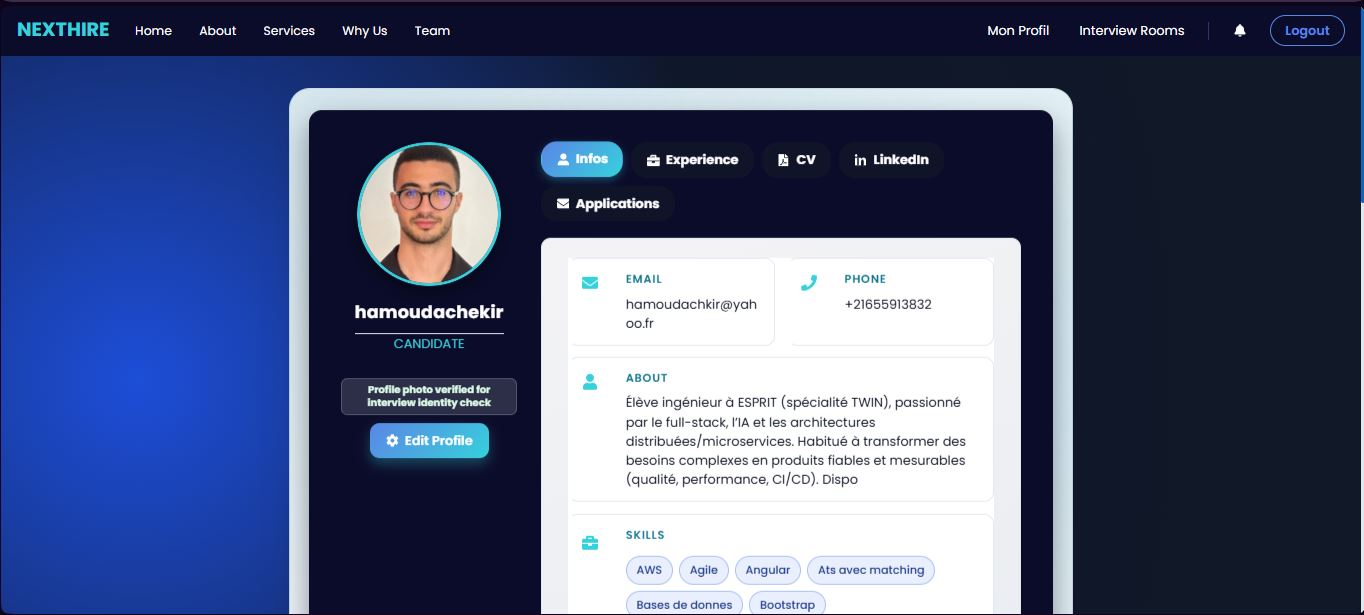
\includegraphics[width=0.48\textwidth,keepaspectratio]{images/profile1.JPG}\hfill
  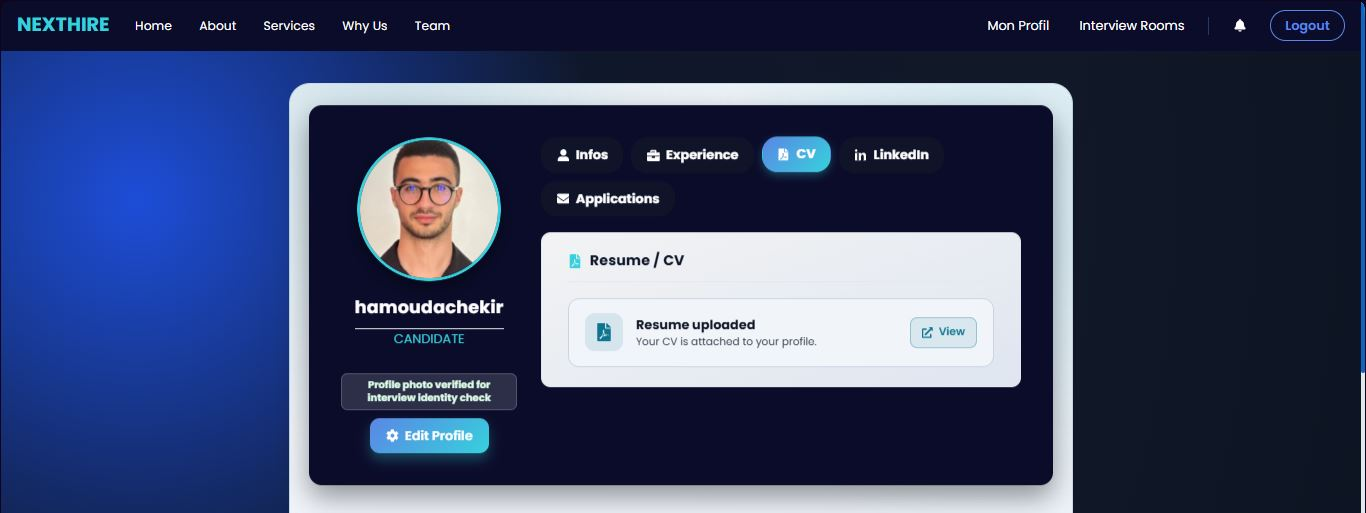
\includegraphics[width=0.48\textwidth,keepaspectratio]{images/profile2.JPG}\\[6pt]
  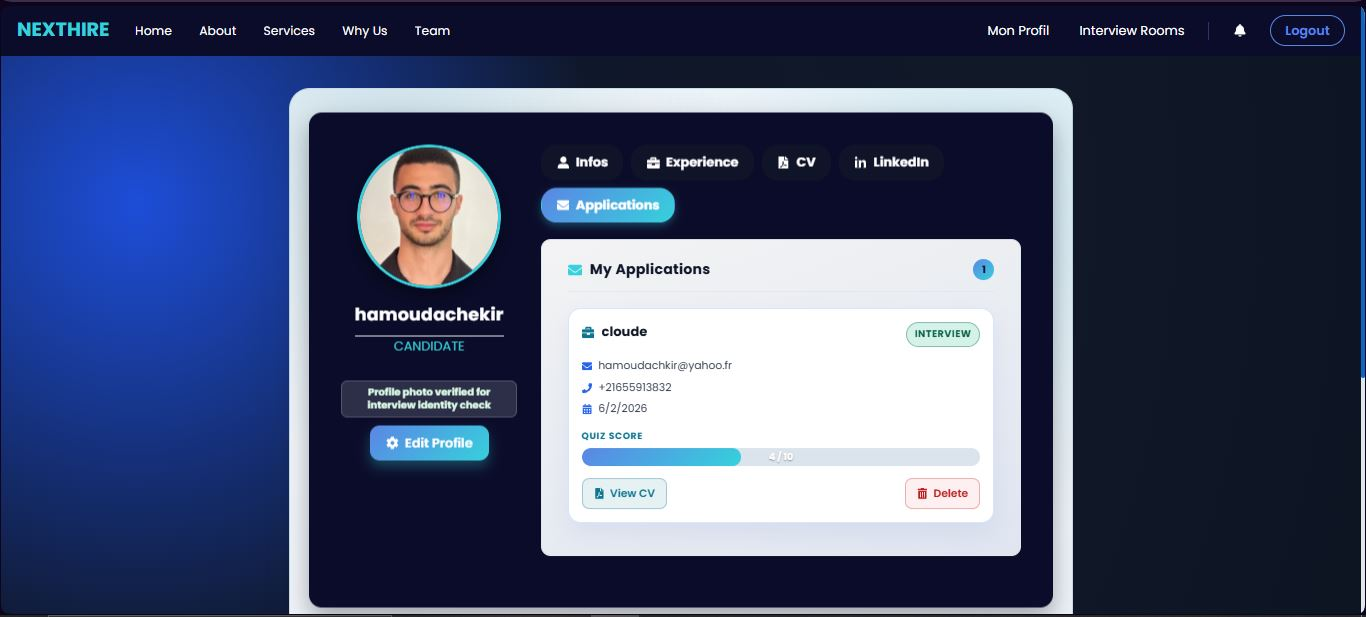
\includegraphics[width=0.75\textwidth,keepaspectratio]{images/profile3.JPG}
  \caption{Écran de profil et tableau de bord du candidat.}
  \label{fig:candidate-profile}
\end{figure}

\subsubsection{Téléversement du CV et profil structuré}

Depuis son profil, le candidat téléverse son CV (PDF ou image). Le fichier est transmis au micro-service d'analyse décrit précédemment, qui en extrait automatiquement un profil structuré : identité, compétences, langues, expériences et formation. Le candidat peut ensuite vérifier et compléter les informations détectées avant de postuler (figure~\ref{fig:cv-upload}).

\begin{figure}[H]
  \centering
  \screenshot{cv-upload.JPG}{Téléversement du CV et profil extrait automatiquement}
  \caption{Téléversement du CV et profil structuré extrait automatiquement.}
  \label{fig:cv-upload}
\end{figure}

\subsubsection{Liaison du compte LinkedIn}

En complément du CV, le candidat peut relier son compte LinkedIn à son profil. Un service d'enrichissement récupère ses données professionnelles publiques et complète automatiquement les compétences et expériences détectées, ce qui améliore la qualité de la présélection et des recommandations (figure~\ref{fig:linkedin}).

\begin{figure}[H]
  \centering
  \screenshot{linkedin-enrichment.JPG}{Liaison du compte LinkedIn et enrichissement du profil}
  \caption{Liaison du compte LinkedIn et enrichissement automatique du profil.}
  \label{fig:linkedin}
\end{figure}

\subsubsection{Page d'accueil et recommandation d'offres}

Dès sa connexion, le candidat arrive sur une page d'accueil qui met en avant une liste
d'offres recommandées personnalisées (figure~\ref{fig:candidate-home}). Le \textit{front-end}
React interroge la route \texttt{GET /recommendation/for-user}, qui relaie la requête au
micro-service de recommandation Python (port~5001) décrit au chapitre~\ref{ch:sprint0} (Sprint~0). Pour la page
d'accueil, le backend demande jusqu'à dix offres (\texttt{top\_k}~=~10) avec un seuil de
similarité abaissé à $0{,}2$ (au lieu de $0{,}3$ par défaut), afin d'élargir l'éventail
d'offres proposées au candidat.

Chaque offre est restituée avec son score de correspondance (\texttt{match\_score}) issu du
score hybride, et les informations de l'entreprise (nom, logo) sont jointes en une seule
requête à la base de données pour enrichir l'affichage. Les offres auxquelles le candidat a
déjà postulé sont automatiquement écartées par le service de recommandation. Le candidat peut
alors consulter le détail d'une offre et postuler directement depuis cette page. Pour préserver
la robustesse de l'interface, l'API se comporte de façon dégradée : si le service de
recommandation est momentanément indisponible, elle renvoie une liste vide plutôt qu'une
erreur, et la page d'accueil reste fonctionnelle.

\begin{figure}[H]
  \centering
  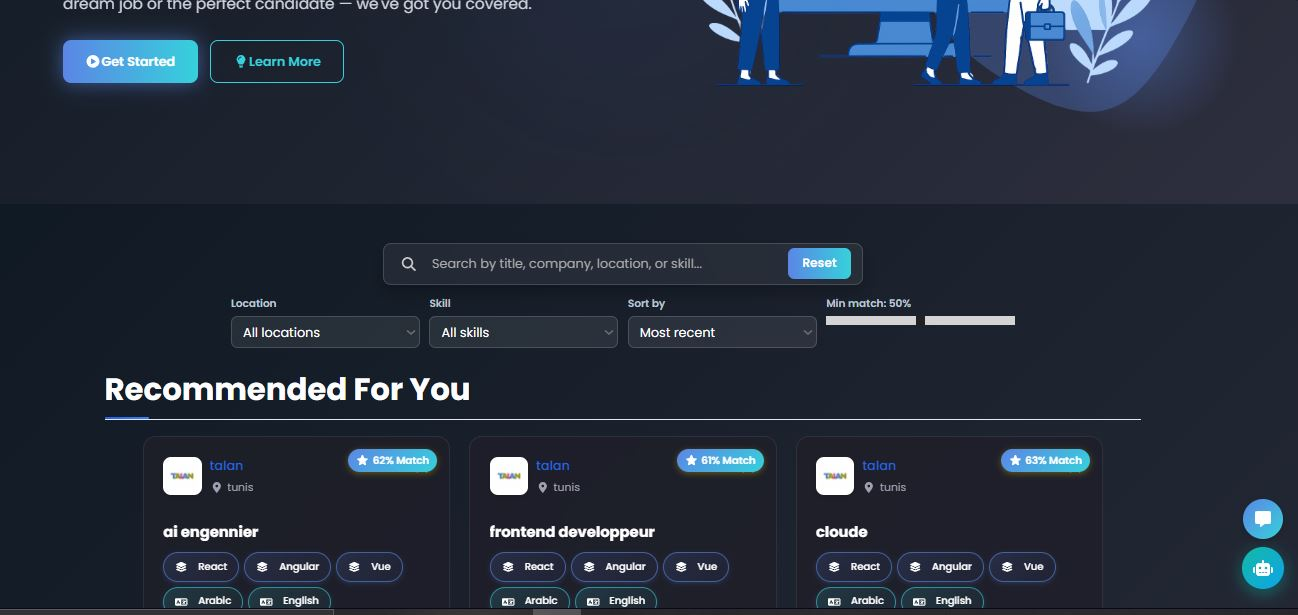
\includegraphics[width=0.9\textwidth,keepaspectratio]{images/home.JPG}
  \caption{Page d'accueil candidat avec les offres recommandées.}
  \label{fig:candidate-home}
\end{figure}

\subsubsection{Quiz de présélection}

Avant d'accéder à l'entretien, le candidat doit réussir le quiz de présélection généré pour sa candidature. Le questionnaire, personnalisé et généré automatiquement par l'IA dès la candidature à partir des compétences attendues pour le poste et de celles du candidat, présente une série de questions (QCM, vrai/faux, réponse courte, mini-exercice) à durée limitée~; le nombre de tentatives est plafonné par un limiteur de débit. Le score obtenu conditionne l'accès à l'étape suivante (figure~\ref{fig:quiz-candidat}).

\begin{figure}[H]
  \centering
  \screenshot{quiz-candidat.JPG}{Passage du quiz de présélection côté candidat}
  \caption{Passage du quiz de présélection par le candidat.}
  \label{fig:quiz-candidat}
\end{figure}

\subsection{Écrans recruteur}

\subsubsection{Tableau de bord recruteur}

L'espace recruteur (route \texttt{/entreprise/:id}, composant \texttt{EntrepriseProfile})
présente les offres d'emploi publiées par l'entreprise, le nombre de candidatures par offre
et la liste des candidats associés. Le recruteur peut y créer ou modifier une offre grâce à
l'assistant de création (\textit{Job Wizard}), suivre l'avancement des candidatures et
accéder au profil de chaque candidat (figure~\ref{fig:recruiter-dashboard}).

\begin{figure}[H]
  \centering
  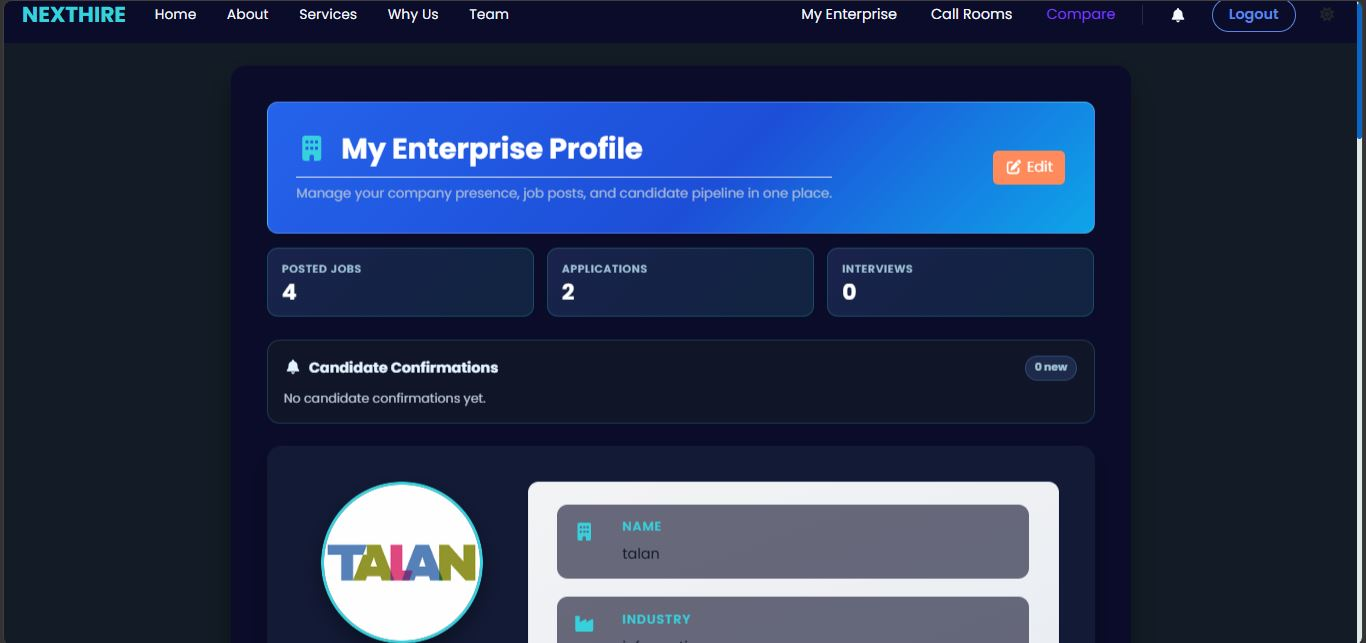
\includegraphics[width=0.9\textwidth,keepaspectratio]{../screenshoot/profilentre.JPG}\\[6pt]
  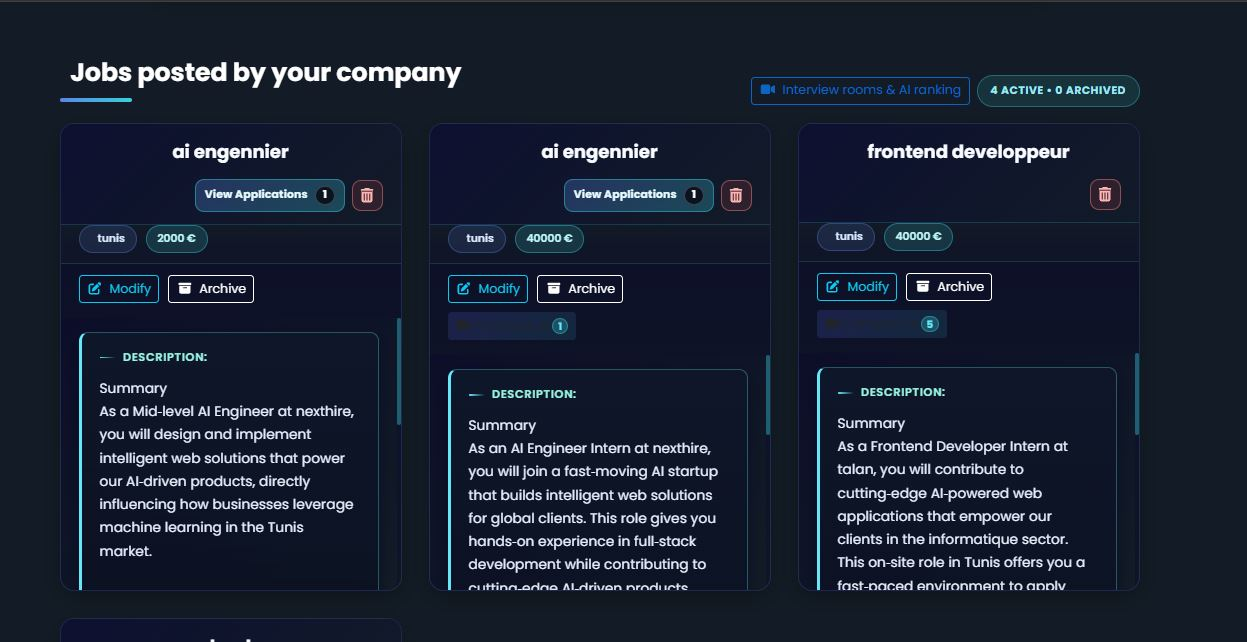
\includegraphics[width=0.9\textwidth,keepaspectratio]{../screenshoot/profjiob.JPG}
  \caption{Tableau de bord recruteur avec vue des offres et des candidatures.}
  \label{fig:recruiter-dashboard}
\end{figure}

\subsubsection{Création d'une offre avec le Job Wizard}

La création d'une offre s'effectue via l'assistant de création (\textit{Job Wizard}), un parcours guidé en plusieurs étapes assisté par l'IA. Le recruteur y renseigne le titre, la description, les compétences requises et le niveau de séniorité~; l'assistant propose des suggestions de contenu et configure les critères d'évaluation pondérés de l'entretien. Le quiz de présélection n'intervient pas à cette étape~: il sera généré automatiquement, par candidat, au moment où celui-ci postule à l'offre (figure~\ref{fig:job-wizard}).

\begin{figure}[H]
  \centering
  \screenshot{job-wizard.JPG}{Assistant de création d'offre (Job Wizard) assisté par IA}
  \caption{Création d'une offre d'emploi via l'assistant \textit{Job Wizard}.}
  \label{fig:job-wizard}
\end{figure}

\section{Tests}

À ce stade du projet, la validation s'est appuyée sur des tests manuels des points de terminaison REST réalisés avec Postman~: création de compte, connexion par JWT, téléversement et analyse de CV, génération des recommandations d'offres et publication d'une offre côté recruteur. Le parcours d'inscription et de complétion de profil a par ailleurs été vérifié de bout en bout dans le navigateur. Les suites de tests automatisées, mutualisées à l'échelle de la plateforme, sont présentées au chapitre~\ref{ch:sprint5} (Sprint~5).

\section{Conclusion}

Ce sprint a livré un socle fonctionnel~: inscription, authentification, analyse de CV, recommandation d'offres et quiz de présélection, ainsi que les premiers espaces candidat et recruteur. Conformément au cadre Scrum, cet incrément a été démontré à nos encadrantes lors de la revue de sprint~; la rétrospective a notamment mis en évidence la grande hétérogénéité des CV réels, ce qui a conduit à renforcer le pipeline d'extraction (reconstruction par colonnes, repli OCR) et à constituer des jeux d'essai plus variés pour les sprints suivants. Le sprint suivant s'appuie sur ces fondations pour introduire la planification des entretiens et la première version de la salle d'entretien en temps réel.
          % Ch2 : Sprint 1 -- Socle de présélection
    \chapter[Sprint 2 : Salle d'entretien temps réel]{Sprint 2 : Une salle d'entretien temps réel\\et la planification des sessions}
\begin{spacing}{1.2}
\minitoc%
\thispagestyle{MyStyle}
\end{spacing}
\clearpage

\providecommand{\screenshot}[2]{%
  \IfFileExists{../screenshoot/#1}{%
    \includegraphics[width=0.9\textwidth,height=12cm,keepaspectratio]{../screenshoot/#1}%
  }{%
    \fbox{\parbox[c][4.5cm][c]{0.9\textwidth}{\centering\itshape
      Capture d'écran à insérer~: #2\\[4pt]
      \normalfont\small(fichier attendu~: \texttt{screenshoot/#1})}}%
  }%
}

\section{Introduction}

Ce chapitre détaille le Sprint~2, consacré à la dimension temps réel de la plateforme NextHire. Il couvre l'ensemble du parcours qui conduit un candidat présélectionné jusqu'à un entretien en direct~: la planification de la rencontre, la création et la jonction d'une salle d'entretien sécurisée, puis l'établissement d'une communication audio et vidéo synchrone entre le candidat et le recruteur. Le chapitre présente successivement les objectifs et le backlog du sprint, le concept de la salle d'entretien synchrone, sa conception détaillée illustrée par des diagrammes de séquence, puis les interfaces réalisées.

\section{Objectifs du sprint}

L'objectif principal de ce sprint est défini comme suit~:

\begin{quote}
\itshape Doter NextHire d'un canal d'entretien synchrone~: permettre à un candidat de planifier son entretien, de rejoindre une salle d'entretien sécurisée et d'y dialoguer en direct avec le recruteur, grâce à une communication temps réel fondée sur WebRTC et Socket.IO.
\end{quote}

\subsection{Backlog du sprint}

Pour atteindre cet objectif, un sous-ensemble du \textit{product backlog} a été sélectionné puis affiné en récits utilisateurs et tâches techniques, afin de constituer le backlog du Sprint~2 (tableau~\ref{tab:backlog-s2}). Comme pour le \textit{product backlog}, chaque élément est priorisé selon la méthode \textbf{MoSCoW} (\textbf{Must}, \textbf{Should}, \textbf{Could}) et estimé en \textit{story points} sur la suite de Fibonacci (1, 2, 3, 5, 8, 13), soit un engagement de 46~points pour ce sprint.

\begin{table}[H]
  \centering
  \footnotesize
  \renewcommand{\arraystretch}{1.3}
  \setlength{\tabcolsep}{5pt}
  \begin{tabularx}{\textwidth}{|>{\centering\arraybackslash}p{1.1cm}|>{\raggedright\arraybackslash}X|>{\centering\arraybackslash}p{1.7cm}|>{\centering\arraybackslash}p{0.9cm}|}
    \hline
    \rowcolor{blue!10}
    \textbf{ID} & \textbf{Récit utilisateur / tâche} & \textbf{Priorité} & \textbf{Est.} \\
    \hline
    T-02 & Mettre en place le micro-service de planification (FastAPI) intégré au calendrier Google (OAuth~2.0) et à l'envoi de courriels de confirmation. & Must & 8 \\
    \hline
    T-03 & Établir l'infrastructure de communication temps réel~: serveur de signalisation Socket.IO et échange de flux audio/vidéo WebRTC. & Must & 8 \\
    \hline
    S1 & En tant que recruteur, je veux lancer la planification et proposer au candidat des créneaux issus de mon calendrier Google. & Must & 5 \\
    \hline
    S2 & En tant que candidat, je veux choisir l'un des créneaux proposés afin de confirmer mon entretien, avec notification automatique par courriel. & Must & 3 \\
    \hline
    S3 & En tant que recruteur, je veux créer une salle d'entretien partageable associée à un poste et à un candidat. & Must & 3 \\
    \hline
    S4 & En tant que candidat, je veux consulter en temps réel les salles d'entretien disponibles et demander à en rejoindre une. & Must & 5 \\
    \hline
    S5 & En tant que recruteur, je veux admettre le candidat dans la salle et démarrer la session d'entretien en direct. & Must & 3 \\
    \hline
    S6 & En tant que participant, je veux dialoguer en audio et vidéo en direct dans la salle, les changements d'état de la session étant diffusés en temps réel à tous les participants. & Must & 8 \\
    \hline
    T-04 & Améliorer les interfaces des espaces candidat et recruteur (planification, liste des salles, salle d'entretien en direct). & Should & 3 \\
    \hline
  \end{tabularx}
  \caption{Backlog du Sprint~2 : planification et salle d'entretien temps réel.}
  \label{tab:backlog-s2}
\end{table}

\section{Concept de la salle d'entretien synchrone}

\subsection{De l'entretien asynchrone à l'entretien synchrone}

La plupart des plateformes de recrutement assisté par l'IA reposent sur l'entretien vidéo \textit{asynchrone}~: le candidat répond seul, face à son écran, à des questions préenregistrées. NextHire fait le choix inverse d'un entretien \textit{synchrone}, conduit en direct dans une salle partagée. Cette salle réunit le candidat et le recruteur (puis, au sprint suivant, l'agent d'entretien vocal) au sein d'une même session, où chaque action (question, réponse, transcription, changement d'état) est diffusée à tous les participants en temps réel. Ce parti pris rend l'échange plus humain et permet une évaluation adaptative, mais impose une infrastructure temps réel robuste, objet de ce sprint.

\subsection{Cycle de vie d'une session d'entretien}

Chaque session est matérialisée par une entité \texttt{CallRoom} qui suit un cycle de vie clair, piloté par deux rôles~:

\begin{itemize}
  \item \textbf{L'hôte (recruteur)} crée la salle pour un poste et un candidat donnés, puis admet le candidat et démarre la session.
  \item \textbf{Le participant (candidat)} découvre la salle dans la liste des salles disponibles, demande à la rejoindre, puis y accède une fois admis.
\end{itemize}

La salle traverse trois états successifs~: \textbf{en attente} (\textit{waiting}, salle créée mais candidat non encore admis), \textbf{active} (entretien en cours) et \textbf{terminée} (\textit{ended}). Chaque transition est diffusée en temps réel à l'ensemble des participants via Socket.IO.

\section{Conception détaillée et architecture}

La conception de ce sprint s'appuie sur les trois protocoles complémentaires présentés au chapitre~\ref{ch:sprint0} (Sprint~0)~: REST pour les opérations CRUD, Socket.IO pour la signalisation et les échanges en temps réel, et WebRTC pour les flux audio et vidéo pair-à-pair. Les trois sections suivantes détaillent les principaux flux, planification, création et jonction de la salle, établissement de la connexion temps réel, chacun illustré par un diagramme de séquence.

\subsection{Planification des entretiens}

La planification est assurée par un micro-service Python (FastAPI, port~5004) dédié. À partir des disponibilités du recruteur, lues dans son calendrier Google, le service \textbf{génère et classe des créneaux proposés}, puis transmet au candidat un lien de confirmation par courriel. Lorsque le candidat retient l'un de ces créneaux, le service crée l'événement correspondant dans Google Calendar (API OAuth~2.0), notifie les deux parties, puis avertit le BFF Node.js par une route interne. La figure~\ref{fig:seq-scheduling} illustre ce flux.

\begin{figure}[H]
  \centering
  \resizebox{\textwidth}{!}{%
  \begin{tikzpicture}[
    font=\scriptsize, >={Stealth[length=2mm]},
    msg/.style={->, thin},
    ret/.style={->, thin, dashed},
    lbl/.style={font=\tiny, fill=white, inner sep=1pt, midway, above},
    lifeline/.style={dashed, thin, gray!70},
    phdr/.style={draw, fill=blue!12, rounded corners=2pt, align=center,
                 font=\scriptsize\bfseries, minimum height=0.7cm, minimum width=2.6cm},
  ]
    \node[phdr] at ( 0,0) {Recruteur\\(React)};
    \node[phdr] at ( 5,0) {Node BFF\\(:3001)};
    \node[phdr] at (10,0) {Scheduling\\(:5004)};
    \node[phdr] at (15,0) {Google Calendar\\+ SMTP};
    \node[phdr] at (19.5,0) {Candidat\\(courriel/React)};
    \foreach \x in {0,5,10,15,19.5}{ \draw[lifeline] (\x,-0.42) -- (\x,-9.8); }

    \draw[msg] ( 0,-0.85) -- node[lbl] {lancer la planification \{candidat, poste\}} (5,-0.85);
    \draw[msg] ( 5,-1.55) -- node[lbl] {POST /api/scheduling/start} (10,-1.55);
    \draw[msg] (10,-2.25) -- node[lbl] {lire les disponibilités du recruteur} (15,-2.25);
    \draw[ret] (15,-2.95) -- node[lbl] {\{créneaux occupés\}} (10,-2.95);
    \draw[->] (10,-3.45) -- ++(0.55,0) -- ++(0,-0.4) -- ++(-0.55,0);
    \node[font=\tiny, anchor=west] at (10.65,-3.65) {générer et classer les créneaux proposés};
    \draw[msg] (10,-4.35) -- node[lbl] {courriel : lien de confirmation} (19.5,-4.35);

    \draw[draw=gray!55, fill=gray!8, rounded corners=2pt, thin] (8.5,-4.8) rectangle (19.0,-5.25);
    \node[font=\tiny, anchor=west] at (8.6,-5.02) {Le candidat ouvre le lien et choisit un créneau};

    \draw[msg] (19.5,-5.65) -- node[lbl] {GET /api/scheduling/public/\{token\}} (10,-5.65);
    \draw[ret] (10,-6.35) -- node[lbl] {\{créneaux proposés\}} (19.5,-6.35);
    \draw[msg] (19.5,-7.05) -- node[lbl] {POST /api/scheduling/public/\{token\}/confirm} (10,-7.05);
    \draw[msg] (10,-7.75) -- node[lbl] {créer l'événement} (15,-7.75);
    \draw[ret] (15,-8.45) -- node[lbl] {\{eventLink\}} (10,-8.45);
    \draw[msg] (10,-9.15) -- node[lbl] {notifier les deux parties (courriels)} (15,-9.15);
    \draw[ret] (10,-9.65) -- node[lbl] {callback /internal/scheduling/candidate-confirmation} (5,-9.65);
  \end{tikzpicture}}
  \caption{Diagramme de séquence : planification d'un entretien (créneaux proposés au candidat).}
  \label{fig:seq-scheduling}
\end{figure}

\subsection{Création et jonction d'une salle d'entretien}

Le cycle de vie d'une session est piloté par le routeur \texttt{callRoom} en coordination avec \texttt{interviewRoute}. Le recruteur crée une salle, qui apparaît instantanément dans la liste des salles disponibles des candidats concernés~; le candidat demande à la rejoindre, et le recruteur confirme son admission. Les principaux points de terminaison sont~:

\begin{itemize}
  \item \texttt{POST /api/call-rooms/create} crée une nouvelle salle d'entretien pour un candidat et un poste donnés.
  \item \texttt{GET /api/call-rooms/available} retourne la liste des salles d'entretien ouvertes pour le candidat.
  \item \texttt{GET /api/call-rooms/:roomId} retourne le contexte complet de la session (profil candidat, exigences du poste, statut).
\end{itemize}

\noindent La signalisation temps réel s'appuie sur les événements Socket.IO émis par les clients (\texttt{call-\allowbreak room-\allowbreak created}, \texttt{call-\allowbreak room-\allowbreak join-\allowbreak request}, \texttt{confirm-\allowbreak candidate-\allowbreak join}), que le serveur relaie sous des noms dédiés (\texttt{new-\allowbreak call-\allowbreak room}, \texttt{candidate-\allowbreak join-\allowbreak request}, \texttt{join-\allowbreak confirmed}), ainsi que sur \texttt{call-\allowbreak room-\allowbreak status-\allowbreak update} pour la mise à jour de la liste des salles disponibles. La figure~\ref{fig:seq-room} en présente l'enchaînement.

\begin{figure}[H]
  \centering
  \resizebox{\textwidth}{!}{%
  \begin{tikzpicture}[
    font=\scriptsize, >={Stealth[length=2mm]},
    msg/.style={->, thin},
    ret/.style={->, thin, dashed},
    lbl/.style={font=\tiny, fill=white, inner sep=1pt, midway, above},
    lifeline/.style={dashed, thin, gray!70},
    phdr/.style={draw, fill=blue!12, rounded corners=2pt, align=center,
                 font=\scriptsize\bfseries, minimum height=0.7cm, minimum width=3.0cm},
  ]
    \node[phdr] at ( 0,0) {Recruteur\\(React)};
    \node[phdr] at ( 6,0) {Node BFF\\Socket.IO :3001};
    \node[phdr] at (11,0) {MongoDB};
    \node[phdr] at (16,0) {Candidat\\(React)};
    \foreach \x in {0,6,11,16}{ \draw[lifeline] (\x,-0.42) -- (\x,-8.6); }

    \draw[msg] ( 0,-0.85) -- node[lbl] {POST /call-rooms/create \{jobId, candidateId\}} (6,-0.85);
    \draw[msg] ( 6,-1.55) -- node[lbl] {insert CallRoom \{status: waiting\}} (11,-1.55);
    \draw[ret] (11,-2.25) -- node[lbl] {\{roomId\}} (6,-2.25);
    \draw[ret] ( 6,-2.95) -- node[lbl] {\{roomId, status: waiting\}} (0,-2.95);
    \draw[msg] ( 6,-3.65) -- node[lbl] {emit "call-room-created"} (16,-3.65);
    \draw[ret] ( 6,-4.0) -- node[lbl, font=\tiny] {relayé "new-call-room"} (16,-4.0);
    \draw[msg] (16,-4.65) -- node[lbl] {emit "call-room-join-request" \{roomId\}} (6,-4.65);
    \draw[msg] ( 6,-5.35) -- node[lbl] {relayé "candidate-join-request"} (0,-5.35);
    \draw[msg] ( 0,-6.05) -- node[lbl] {emit "confirm-candidate-join"} (6,-6.05);
    \draw[msg] ( 6,-6.75) -- node[lbl] {update CallRoom \{status: active\}} (11,-6.75);
    \draw[ret] ( 6,-7.45) -- node[lbl] {relayé "join-confirmed" $\rightarrow$ redirection} (16,-7.45);
    \draw[ret] ( 6,-8.15) -- node[lbl] {emit "call-room-status-update" \{active\}} (0,-8.15);
  \end{tikzpicture}}
  \caption{Diagramme de séquence : création et jonction d'une salle d'entretien.}
  \label{fig:seq-room}
\end{figure}

\subsection{Signalisation temps réel et établissement WebRTC}

Une fois le candidat admis, la connexion média est négociée par échange de signalisation via Socket.IO~: les deux pairs s'échangent leurs descriptions de session (offre et réponse SDP) puis leurs candidats ICE, le serveur Node se limitant à relayer ces messages entre les deux clients sans jamais y accéder. Une fois la négociation terminée, le flux audio et vidéo circule directement en pair-à-pair entre le candidat et le recruteur, sans transiter par le serveur. La figure~\ref{fig:seq-webrtc} détaille cet établissement.

\begin{figure}[H]
  \centering
  \resizebox{0.92\textwidth}{!}{%
  \begin{tikzpicture}[
    font=\scriptsize, >={Stealth[length=2mm]},
    msg/.style={->, thin},
    ret/.style={->, thin, dashed},
    lbl/.style={font=\tiny, fill=white, inner sep=1pt, midway, above},
    lifeline/.style={dashed, thin, gray!70},
    phdr/.style={draw, fill=blue!12, rounded corners=2pt, align=center,
                 font=\scriptsize\bfseries, minimum height=0.7cm, minimum width=3.0cm},
  ]
    \node[phdr] at ( 0,0) {Candidat\\(React)};
    \node[phdr] at ( 7,0) {Node\\Socket.IO :3001};
    \node[phdr] at (14,0) {Recruteur\\(React)};
    \foreach \x in {0,7,14}{ \draw[lifeline] (\x,-0.42) -- (\x,-9.4); }

    \draw[msg] ( 0,-0.85) -- node[lbl] {emit "join-interview" \{interviewId\}} (7,-0.85);
    \draw[msg] ( 7,-1.55) -- node[lbl] {emit "user-connected"} (14,-1.55);
    \draw[msg] (14,-2.25) -- node[lbl] {emit "offer" \{SDP\}} (7,-2.25);
    \draw[msg] ( 7,-2.95) -- node[lbl] {relais "offer" \{SDP\}} (0,-2.95);
    \draw[msg] ( 0,-3.65) -- node[lbl] {emit "answer" \{SDP\}} (7,-3.65);
    \draw[msg] ( 7,-4.35) -- node[lbl] {relais "answer" \{SDP\}} (14,-4.35);

    \draw[draw=green!50!black, fill=green!5, rounded corners=3pt, dashed, thin]
      (-0.4,-4.8) rectangle (14.4,-6.5);
    \node[font=\tiny\bfseries, text=green!40!black, anchor=north west] at (-0.3,-4.85)
      {loop [échange des candidats ICE]};
    \draw[msg] ( 0,-5.55) -- node[lbl] {emit "ice-candidate"} (7,-5.55);
    \draw[msg] ( 7,-6.15) -- node[lbl] {relais "ice-candidate"} (14,-6.15);

    \draw[<->, very thick, green!45!black] (0,-7.1) -- node[font=\tiny, fill=white, midway]
      {Connexion P2P établie : flux audio/vidéo (WebRTC)} (14,-7.1);
    \draw[msg] ( 7,-8.0) -- node[lbl] {diffusion de l'état de la salle (Socket.IO)} (0,-8.0);
    \draw[msg] ( 7,-8.7) -- node[lbl] {diffusion de l'état de la salle (Socket.IO)} (14,-8.7);
  \end{tikzpicture}}
  \caption{Diagramme de séquence : signalisation et établissement de la connexion WebRTC.}
  \label{fig:seq-webrtc}
\end{figure}

\section{Réalisation et interfaces utilisateur}

Cette section présente les interfaces réalisées au cours du sprint, en suivant le parcours d'un entretien~: planification, création de la salle, accès du candidat, puis entretien en direct.

\subsection{Planification de l'entretien}

Côté recruteur, l'interface de planification permet de lancer la planification et de proposer au candidat des créneaux issus de son calendrier Google (figure~\ref{fig:scheduling-ui}). Le candidat retient ensuite l'un des créneaux depuis le lien reçu par courriel~; sa confirmation déclenche la création de l'événement Google Calendar et l'envoi des courriels de notification aux deux parties.

\begin{figure}[H]
  \centering
  \screenshot{scheduling.JPG}{Planification : proposition et confirmation d'un créneau}
  \caption{Interface de planification d'un entretien côté recruteur.}
  \label{fig:scheduling-ui}
\end{figure}

\subsection{Création de la salle d'entretien}

Le recruteur crée une salle d'entretien associée à un poste~; cette opération génère la session \texttt{CallRoom} partagée et la rend visible aux candidats concernés. Avant le démarrage, les participants se retrouvent dans une salle d'attente (\textit{lobby}), où le recruteur admet le candidat (figure~\ref{fig:room-creation}).

\begin{figure}[H]
  \centering
  \screenshot{room-creation.JPG}{Création d'une salle d'entretien et salle d'attente}
  \caption{Création d'une salle d'entretien et salle d'attente (\textit{lobby}).}
  \label{fig:room-creation}
\end{figure}

\subsection{Salles d'entretien disponibles}

Le candidat dispose d'un écran listant les salles d'entretien disponibles auxquelles il peut se joindre (figure~\ref{fig:available-rooms}), alimenté par la route \texttt{GET /api/call-rooms/available}. Cette liste se met à jour en temps réel grâce à Socket.IO~: lorsqu'un recruteur ouvre une nouvelle salle, celle-ci apparaît instantanément chez les candidats concernés, et toute salle clôturée ou déjà démarrée en est retirée automatiquement. Pour rejoindre un entretien, le candidat envoie une demande (\texttt{call-room-join-request}) puis attend la confirmation du recruteur~; dès que celle-ci est reçue, il est redirigé automatiquement vers la salle. Un mécanisme de secours par interrogation périodique assure cette redirection même si l'événement temps réel venait à être manqué.

\begin{figure}[H]
  \centering
  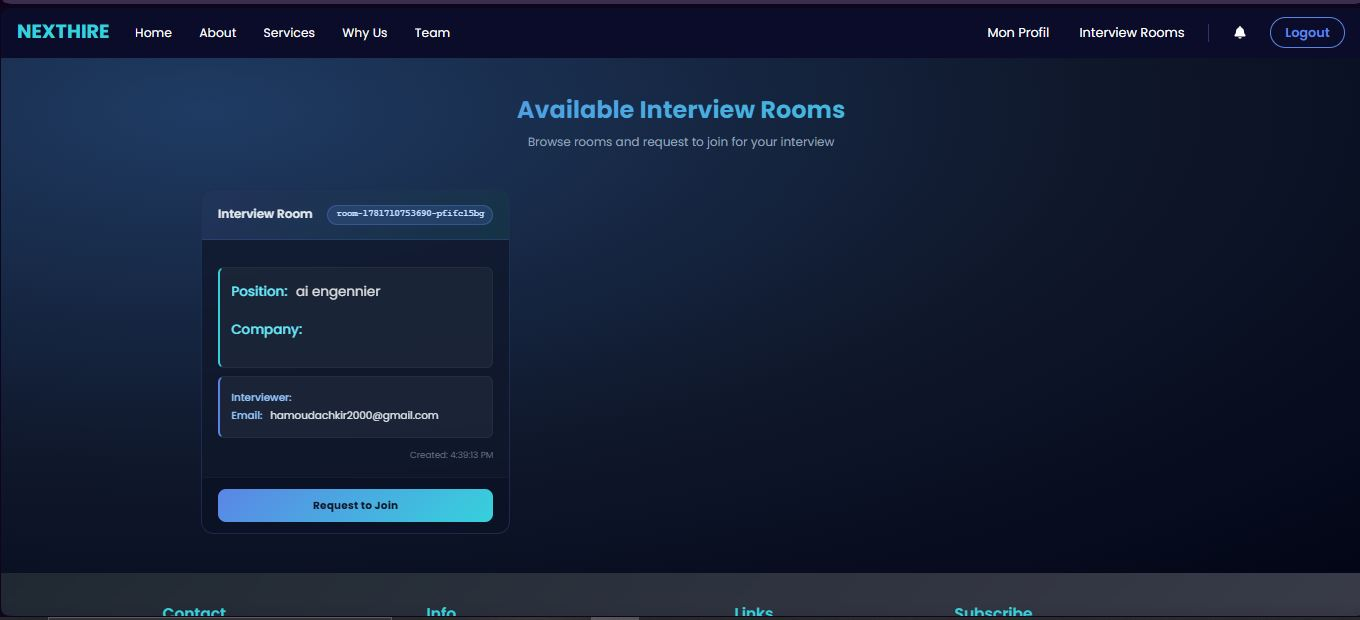
\includegraphics[width=0.9\textwidth,keepaspectratio]{images/available-room.JPG}
  \caption{Liste des salles d'entretien disponibles pour le candidat.}
  \label{fig:available-rooms}
\end{figure}

\subsection{La salle d'entretien en direct}

Une fois le candidat admis, les deux participants se retrouvent dans la salle d'entretien en direct. Les flux audio et vidéo circulent en pair-à-pair grâce à WebRTC, tandis que l'état de la salle et les échanges sont synchronisés en temps réel via Socket.IO (figure~\ref{fig:callroom}). Le pipeline vocal et l'agent d'entretien adaptatif y seront intégrés au sprint suivant.

\begin{figure}[H]
  \centering
  \screenshot{callroom.JPG}{Salle d'entretien temps réel (audio/vidéo WebRTC)}
  \caption{La salle d'entretien en direct entre le candidat et le recruteur.}
  \label{fig:callroom}
\end{figure}

\section{Tests}

La validation de ce sprint a porté sur l'intégration du module de planification (création d'événements Google Calendar et envoi des courriels de confirmation) et sur la signalisation WebRTC/Socket.IO de la salle d'entretien, vérifiée manuellement avec deux clients connectés simultanément (un candidat, un recruteur)~: création de la salle, demande et confirmation de jonction, puis établissement de la connexion audio/vidéo. Les tests automatisés de bout en bout du parcours recruteur sont présentés au chapitre~\ref{ch:sprint5} (Sprint~5).

\section{Conclusion}

Ce sprint a doté NextHire d'un canal d'entretien synchrone complet~: planification intégrée au calendrier, création et jonction d'une salle d'entretien sécurisée, et établissement d'une communication audio et vidéo temps réel entre le candidat et le recruteur. La revue de sprint a permis de dérouler le parcours complet, de la planification jusqu'à la salle en direct, devant nos encadrantes~; la rétrospective a souligné le coût de mise au point de la signalisation WebRTC (traversée NAT, permissions médias), d'où la décision de tester systématiquement les fonctionnalités temps réel sur plusieurs navigateurs et conditions réseau dès les sprints suivants. Le sprint suivant exploite cette salle pour y faire intervenir l'agent d'entretien vocal adaptatif, cœur fonctionnel de la plateforme.
          % Ch3 : Sprint 2 -- Salle d'entretien
    \chapter[Sprint 3 : Agent vocal adaptatif]{Sprint 3 : Un agent d'entretien vocal\\adaptatif piloté par LLM}
\begin{spacing}{1.2}
\minitoc
\thispagestyle{MyStyle}
\end{spacing}
\clearpage

\providecommand{\screenshot}[2]{%
  \IfFileExists{../screenshoot/#1}{%
    \includegraphics[width=0.9\textwidth,height=12cm,keepaspectratio]{../screenshoot/#1}%
  }{%
    \fbox{\parbox[c][4.5cm][c]{0.9\textwidth}{\centering\itshape
      Capture d'écran à insérer~: #2\\[4pt]
      \normalfont\small(fichier attendu~: \texttt{screenshoot/#1})}}%
  }%
}

\section{Introduction}

Ce troisième sprint constitue le cœur du projet~: il livre l'agent d'entretien vocal piloté par un grand modèle de langage, son moteur adaptatif IRT-lite et la pile vocale (transcription et synthèse). L'avatar 3D parlant donne un visage à l'assistante d'entretien \textit{Nour} et rend l'échange plus naturel.

\section{Objectifs du sprint}

L'objectif principal de ce sprint est défini comme suit~:

\begin{quote}
\itshape Concevoir et réaliser le cœur conversationnel de NextHire~: un agent d'entretien vocal qui conduit en temps réel un entretien adaptatif, en générant et en évaluant les questions au moyen d'un grand modèle de langage, en ajustant la difficulté au niveau du candidat (IRT-lite) et en s'exprimant par la voix à travers un avatar 3D.
\end{quote}

\subsection{Backlog du sprint}

Le tableau~\ref{tab:backlog-s3} présente le backlog du Sprint~3.

\begin{table}[H]
  \centering
  \footnotesize
  \renewcommand{\arraystretch}{1.3}
  \setlength{\tabcolsep}{5pt}
  \begin{tabularx}{\textwidth}{|>{\centering\arraybackslash}p{1.1cm}|>{\raggedright\arraybackslash}X|>{\centering\arraybackslash}p{1.8cm}|}
    \hline
    \rowcolor{blue!10}
    \textbf{ID} & \textbf{Récit utilisateur} & \textbf{Priorité} \\
    \hline
    S1 & En tant que candidat, je veux passer un entretien vocal en direct mené par un agent IA. & Haute \\
    \hline
    S2 & En tant que candidat, je veux que les questions s'adaptent à mon niveau au fil de l'entretien. & Haute \\
    \hline
    S3 & En tant que candidat, je veux voir et entendre un avatar 3D qui pose les questions (voix et synchronisation labiale). & Haute \\
    \hline
    S4 & En tant que candidat, je veux suivre la transcription de mes réponses en temps réel. & Moyenne \\
    \hline
    S5 & En tant que recruteur, je veux obtenir une évaluation structurée à l'issue de l'entretien. & Haute \\
    \hline
  \end{tabularx}
  \caption{Backlog du Sprint~3 : Agent d'entretien vocal adaptatif.}
  \label{tab:backlog-s3}
\end{table}

\section{Concept de l'entretien vocal adaptatif}

L'entretien de NextHire est conduit par un agent conversationnel unique, l'assistante «~Nour~», pilotée par une machine à états développée sur mesure plutôt que par un \textit{framework} multi-agents. L'entretien se déroule en deux phases successives, une phase RH comportementale puis une phase technique, chacune dotée de son propre \textit{prompt} système.

La phase technique repose sur une sélection adaptative des questions~: à chaque tour, la capacité estimée du candidat ($\theta$) est mise à jour selon une règle IRT-lite, ce qui oriente la difficulté de la question suivante. L'agent ajuste par ailleurs son ton au niveau de stress détecté chez le candidat (normal, chaleureux, rassurant), sans changer d'interlocuteur. Enfin, l'avatar 3D donne un visage à l'agent~: il énonce les questions par synthèse vocale et synchronise le mouvement de ses lèvres avec l'audio.

\section{Conception détaillée et architecture}

\subsection{Le moteur d'entretien}

Le moteur d'entretien (\texttt{InterviewEngine}) est une machine à états Python native, sans dépendance à LangChain ni LangGraph. Il enchaîne plusieurs nœuds, initialisation de session, ouverture, attente de réponse, traitement de la réponse, mise à jour IRT-lite et gestion du stress, génération de la question, puis clôture, autour d'un état partagé \texttt{InterviewState} (configuration du poste, tour courant, capacité estimée $\theta$, niveau de stress). Sa réalisation repose sur un appel JSON unique au LLM Groq (\texttt{openai/gpt-oss-120b}) par tour, qui fusionne l'évaluation de la réponse et la génération de la question suivante, et sur une série de \textit{guards} déterministes traités sans appel LLM (changement de langue, demande de répétition, réponse hors-sujet). L'état de session est conservé dans Redis, avec repli en mémoire en cas d'indisponibilité. La figure~\ref{fig:interview-engine} en présente la machine à états et l'état \texttt{InterviewState} associé.

\begin{figure}[H]
  \centering
  \resizebox{\textwidth}{!}{%
  \begin{tikzpicture}[
    font=\scriptsize,
    >=Stealth,
    box/.style={draw, rounded corners=3pt, fill=blue!10,
                minimum width=3.4cm, minimum height=0.65cm, align=center, font=\tiny},
    io/.style={draw, dashed, rounded corners=3pt, fill=orange!12,
               minimum width=3.4cm, minimum height=0.65cm, align=center, font=\tiny},
    dec/.style={draw, diamond, fill=yellow!15, aspect=2.4, align=center,
                inner sep=1pt, font=\tiny},
    term/.style={draw, ellipse, fill=gray!25, minimum width=1.8cm,
                 minimum height=0.5cm, align=center, font=\tiny\bfseries},
    ann/.style={draw=blue!30, fill=blue!4, align=left, text width=3.9cm,
                inner sep=2.5pt, font=\tiny, rounded corners=2pt},
  ]

  %% ── Main flow (centered at x = 0) ──────────────────────────────────────
  \node[term] (start) at (0,    0)    {START};
  \node[box]  (N0)    at (0,  -1.4)  {initialise\_session};
  \node[box]  (N1)    at (0,  -2.7)  {ouverture};
  \node[io]   (N2)    at (0,  -4.1)  {await\_response};
  \node[box]  (N3)    at (0,  -5.4)  {traitement\_réponse};
  \node[box]  (N4)    at (0,  -6.7)  {update\_irt\_stress};
  \node[dec]  (D1)    at (0,  -8.1)  {should\_end ?};
  \node[dec]  (D2)    at (0,  -9.7)  {switch\_phase ?};
  \node[box]  (N5)    at (0, -11.1)  {generate\_question};
  \node[box]  (N6)    at (5,  -8.1)  {end\_interview};
  \node[term] (endn)  at (5,  -9.3)  {END};

  %% ── Arrows ──────────────────────────────────────────────────────────────
  \draw[->] (start) -- (N0);
  \draw[->] (N0)    -- (N1);
  \draw[->] (N1)    -- (N2);
  \draw[->] (N2)    -- node[right,font=\tiny,fill=white,inner sep=0pt]
                         {transcription STT} (N3);
  \draw[->] (N3)    -- (N4);
  \draw[->] (N4)    -- (D1);
  \draw[->] (D1)    -- node[right,font=\tiny]{Non} (D2);
  \draw[->] (D2)    -- node[right,font=\tiny]{Non} (N5);
  \draw[->] (D1.east) -- node[above,font=\tiny]{Oui} (N6.west);
  \draw[->] (N6)      -- (endn);
  \draw[->] (D2.east) -- ++(0.7,0) |-
            node[right,font=\tiny,pos=0.4]{Oui $\to$ technique}
            (N5.east);
  \draw[->] (N5.south) -- ++(0,-0.45) -- ++(-3.0,0) |- (N2.west);

  %% ── Main Interview Loop bounding box ────────────────────────────────────
  \draw[dashed, draw=gray!55, rounded corners=3pt]
    (-2.1,-3.3) rectangle (2.1,-11.85);
  \node[font=\tiny, text=gray, fill=white, inner sep=1pt]
    at (0,-3.3) {Boucle principale d'entretien};

  %% ── Annotation boxes ─────────────────────────────────────────────────
  \node[ann] at (7.0, -1.4) {
    InterviewState créé\\
    -- interview\_id, job\_title, skills\\
    -- seniority, eval\_criteria, style
  };
  \node[ann] at (7.0, -2.7) {
    Tour 0 : message fixe «Nour»\\
    -- aucun appel LLM
  };
  \node[ann] at (7.0, -4.1) {
    [I/O] Bloquant -- attend\\
    transcription WebSocket\\
    Faster Whisper STT :8012
  };
  \node[ann] at (7.0, -5.4) {
    Guards déterministes OU LLM\\
    Groq $\to$ score, conf., question,\\
    difficulty, skill\_focus, done
  };
  \node[ann] at (7.0, -6.7) {
    IRT-lite : $\theta \mathrel{+}= 0.4(\mathrm{score}{-}0.5)$\\
    \phantom{IRT-lite : }$+\, 0.1(\mathrm{conf.}{-}0.5)$\\
    stress\_level $\to$ agent\_mode\\
    (normal/warm/supportive/reset)
  };
  \node[ann] at (7.0,-11.1) {
    Skill rotation + déduplication\\
    (similarité de tokens $\geq 0.65$), fallback bank
  };
  \node[ann] at (9.8, -9.3) {
    build\_final\_report() :\\
    weighted scores, hiring\_rec\\
    $\to$ POST /call-rooms/:id/end
  };

  %% ── InterviewState panel (top-right) ─────────────────────────────────
  \draw[draw=black!45, rounded corners=3pt, fill=gray!5]
    (8.2, 0.5) rectangle (13.0, -2.8);
  \node[font=\tiny\bfseries] at (10.6, 0.32) {InterviewState (dataclass)};
  \draw[black!30] (8.2,-0.1) -- (13.0,-0.1);
  \node[font=\tiny, align=left, text width=4.4cm] at (10.6,-1.45) {
    \textbf{Session / Config :} interview\_id,\\
    \quad candidate\_name, job\_title, skills,\\
    \quad seniority, evaluation\_criteria,\\
    \quad interview\_style, preferred\_language\\[2pt]
    \textbf{Live Turn :} phase, turn\_index,\\
    \quad theta (IRT), transcript, evaluations,\\
    \quad intro\_question\_count\\[2pt]
    \textbf{Contrôle :} stress\_level,\\
    \quad struggle\_streak, ended
  };

  \end{tikzpicture}%
  }%
  \caption{Machine à états de l'agent d'entretien NextHire
           (\textit{custom Python} -- sans LangGraph/LangChain).}
  \label{fig:interview-engine}
\end{figure}

\subsection{Pile vocale (STT et TTS)}

La pile vocale est portée par un micro-service FastAPI dédié. La transcription des réponses du candidat est assurée en continu par Faster-Whisper, dont le fournisseur et la langue sont sélectionnés selon la configuration de la session. La synthèse vocale de l'assistante \textit{Nour} s'appuie sur Edge TTS, qui fonctionne en \textit{streaming}~: les premiers fragments audio sont émis avant la fin de la synthèse, ce qui réduit la latence perçue. L'audio est diffusé au client via Socket.IO et synchronisé avec le mouvement des lèvres de l'avatar.

\subsection{Flux d'une session d'entretien}

La figure~\ref{fig:seq-interview} illustre le flux de messages d'une session d'entretien IA NextHire, de l'initialisation de la salle jusqu'à la génération du rapport final.

Les étapes clés sont les suivantes.

\begin{sloppypar}
\begin{enumerate}
  \item \textbf{Initialisation.} Le candidat ouvre la page d'entretien. Le client React envoie
        une requête \texttt{GET} vers \texttt{/api/call-rooms/\{roomId\}} au backend Node.js,
        qui récupère le document \texttt{CallRoom} dans MongoDB (contexte du poste, profil
        candidat, statut de la session) et retourne ces données au client.

  \item \textbf{Vérification d'identité.} Le candidat soumet une image de sa webcam pour
        la vérification faciale. Le backend appelle le service Face Verify (Python, port 8011),
        qui compare l'embedding de l'image en direct avec celui enregistré lors de l'inscription
        (similarité cosinus, modèle InsightFace \textit{buffalo-l}) et autorise l'entretien
        si le seuil de correspondance est atteint.

  \item \textbf{Démarrage de l'entretien.} Le client établit une connexion Socket.IO avec le
        backend. Celui-ci initialise une session auprès de l'Interview Agent via REST. L'agent
        crée un objet \texttt{InterviewState} en mémoire, appelle le LLM Groq avec le prompt
        système pour générer la question d'ouverture, transmet le texte à Edge TTS pour la
        synthèse vocale, et diffuse l'audio au candidat.

  \item \textbf{Boucle Q\&A.} Le candidat répond oralement. L'audio PCM est envoyé au backend
        via Socket.IO, transcrit par Faster Whisper (STT), puis transmis à l'Interview Agent.
        L'agent évalue la réponse via le LLM (scoring IRT-lite, mise à jour du score de
        capacité adaptative) et génère la question suivante. La boucle se répète jusqu'à ce
        que le champ \texttt{done} retourné par le LLM soit \texttt{true}.

  \item \textbf{Fin de l'entretien.} L'agent retourne l'évaluation finale avec la transcription
        complète. Le backend construit le rapport recruteur, le persiste dans MongoDB, déclenche
        l'analyse post-entretien en arrière-plan (service Analysis), et notifie le client via
        Socket.IO.
\end{enumerate}
\end{sloppypar}

\begin{figure}[H]
  \centering
  \resizebox{\textwidth}{!}{%
  \begin{tikzpicture}[
    font=\scriptsize,
    >={Stealth[length=2mm]},
    msg/.style={->, thin},
    ret/.style={->, thin, dashed},
    lbl/.style={font=\tiny, fill=white, inner sep=1pt, midway, above},
    lifeline/.style={dashed, thin, gray!70},
    phdr/.style={draw, fill=blue!12, rounded corners=2pt, align=center,
                 font=\scriptsize\bfseries, minimum height=0.65cm, minimum width=2.8cm},
  ]

  %% ── Participant boxes ──────────────────────────────────────────────────
  \node[phdr] at ( 0, 0) {React\\(Client)};
  \node[phdr] at ( 4, 0) {Node.js\\(:3001)};
  \node[phdr] at ( 8, 0) {Interview Agent\\(:8013)};
  \node[phdr] at (12, 0) {Speech Stack\\(STT/TTS :8012)};
  \node[phdr] at (16, 0) {Groq\\(LLM API)};
  \node[phdr] at (20, 0) {MongoDB};
  \node[phdr] at (24, 0) {Analysis Service\\(:8090)};

  %% ── Lifelines ──────────────────────────────────────────────────────────
  \draw[lifeline] ( 0,-0.38) -- ( 0,-21.5);
  \draw[lifeline] ( 4,-0.38) -- ( 4,-21.5);
  \draw[lifeline] ( 8,-0.38) -- ( 8,-21.5);
  \draw[lifeline] (12,-0.38) -- (12,-21.5);
  \draw[lifeline] (16,-0.38) -- (16,-21.5);
  \draw[lifeline] (20,-0.38) -- (20,-21.5);
  \draw[lifeline] (24,-0.38) -- (24,-21.5);

  %% ════════════════════════════════════════════════════════════════════════
  %% 1. Initialisation
  %% ════════════════════════════════════════════════════════════════════════
  \node[font=\tiny\bfseries, anchor=east] at (-0.3,-0.75) {1.};
  \draw[msg] ( 0,-0.75) -- node[lbl] {GET /api/call-rooms/:roomId} (4,-0.75);
  \draw[msg] ( 4,-1.30) -- node[lbl] {findOne(roomId)} (20,-1.30);
  \draw[ret] (20,-1.85) -- node[lbl] {CallRoom \{jobContext, status, candidateInfo\}} (4,-1.85);
  \draw[ret] ( 4,-2.40) -- node[lbl] {200 OK \{roomId, jobContext\}} (0,-2.40);

  %% ════════════════════════════════════════════════════════════════════════
  %% 2. Vérification d'identité faciale
  %% ════════════════════════════════════════════════════════════════════════
  \node[font=\tiny\bfseries, anchor=east] at (-0.3,-2.85) {2.};
  \draw[msg] (0,-2.85) -- node[lbl] {POST /face-verify \{webcam\_frame\}} (4,-2.85);
  \draw[draw=orange!70, fill=orange!8, rounded corners=1pt, thin]
    (4.1,-3.10) rectangle (7.9,-3.65);
  \node[font=\tiny, anchor=west] at (4.2,-3.38)
    {[Face Verify :8011] compare\_embedding};
  \draw[ret] (4,-3.95) -- node[lbl] {\{allowInterview: true, similarity: 0.92\}} (0,-3.95);
  \draw[msg] (4,-4.45) -- node[lbl] {PATCH call-rooms \{faceVerification: matched\}} (20,-4.45);

  %% ════════════════════════════════════════════════════════════════════════
  %% 3. Démarrage de l'entretien
  %% ════════════════════════════════════════════════════════════════════════
  \node[font=\tiny\bfseries, anchor=east] at (-0.3,-4.95) {3.};
  \draw[msg] (0,-4.95) -- node[lbl] {Socket.IO connect(roomId)} (4,-4.95);
  \draw[msg] (4,-5.55) -- node[lbl] {POST /session/start \{jobContext, candidateProfile, style\}} (8,-5.55);
  %% self-arrow: create InterviewState
  \draw[->] (8,-6.15) -- ++(0.6,0) -- ++(0,-0.40) -- ++(-0.6,0);
  \node[font=\tiny, anchor=west] at (8.70,-6.35) {create InterviewState};
  \draw[msg] (8,-6.90) -- node[lbl] {chat.completions(COMPACT\_SYSTEM + opening\_prompt)} (16,-6.90);
  \draw[ret] (16,-7.50) -- node[lbl] {\{next\_question, score:0.5, done:false\}} (8,-7.50);
  \draw[ret] ( 8,-8.05) -- node[lbl] {\{question\_text\}} (4,-8.05);
  \draw[msg] ( 4,-8.55) -- node[lbl] {POST /api/tts \{question\_text\}} (12,-8.55);
  \draw[ret] (12,-9.10) -- node[lbl] {audio stream} (4,-9.10);
  \draw[ret] ( 4,-9.60) -- node[lbl] {emit("agent-audio",\ audio)} (0,-9.60);

  %% ════════════════════════════════════════════════════════════════════════
  %% 4. Boucle Q&A
  %% ════════════════════════════════════════════════════════════════════════
  \node[font=\tiny\bfseries, anchor=east] at (-0.3,-10.1) {4.};
  %% Loop frame
  \draw[draw=green!50!black, fill=green!5, rounded corners=3pt, dashed, thin]
    (-0.3,-10.1) rectangle (21.3,-18.5);
  \node[font=\tiny\bfseries, text=green!40!black, anchor=north west]
    at (-0.2,-10.15) {loop [répéter jusqu'à done = true]};

  \draw[msg] ( 0,-10.75) -- node[lbl] {emit("audio-chunk",\ PCM\_audio)} (4,-10.75);
  \draw[msg] ( 4,-11.35) -- node[lbl] {POST /api/transcribe \{audio\}} (12,-11.35);
  \draw[ret] (12,-11.95) -- node[lbl] {\{text: transcript\}} (4,-11.95);
  \draw[msg] ( 4,-12.55) -- node[lbl] {POST /session/turn \{interview\_id, transcript\}} (8,-12.55);
  %% self-arrow: IRT update
  \draw[->] (8,-13.15) -- ++(0.6,0) -- ++(0,-0.40) -- ++(-0.6,0);
  \node[font=\tiny, anchor=west] at (8.70,-13.35)
    {update\_theta(score,\ confidence) : IRT-lite};
  \draw[msg] ( 8,-13.95) -- node[lbl] {chat.completions(contexte + réponse candidat)} (16,-13.95);
  \draw[ret] (16,-14.55) -- node[lbl] {\{score, next\_question, difficulty, done\}} (8,-14.55);
  \draw[ret] ( 8,-15.15) -- node[lbl] {\{question, score, done\}} (4,-15.15);
  \draw[msg] ( 4,-15.75) -- node[lbl] {POST /api/tts \{next\_question\} [if !done]} (12,-15.75);
  \draw[ret] (12,-16.35) -- node[lbl] {audio stream} (4,-16.35);
  \draw[ret] ( 4,-16.95) -- node[lbl] {emit("agent-audio",\ audio)} (0,-16.95);
  %% guard box
  \draw[draw=gray!50, fill=gray!8, rounded corners=1pt, thin]
    (0.5,-17.75) rectangle (7.5,-18.25);
  \node[font=\tiny] at (4.0,-18.00)
    {[done = true] $\Rightarrow$ sortie de boucle};

  %% ════════════════════════════════════════════════════════════════════════
  %% 5. Fin de l'entretien
  %% ════════════════════════════════════════════════════════════════════════
  \node[font=\tiny\bfseries, anchor=east] at (-0.3,-18.8) {5.};
  \draw[ret] ( 8,-18.80) -- node[lbl] {\{done:true, final\_evaluation, transcript\}} (4,-18.80);
  \draw[msg] ( 4,-19.40) -- node[lbl] {PATCH /call-rooms/:id \{status:ended, recruiterReport\}} (20,-19.40);
  \draw[ret] (20,-19.95) -- node[lbl] {200 OK} (4,-19.95);
  \draw[msg] ( 4,-20.50) -- node[lbl] {POST /api/interviews/:id/analyze-video (async, fire-and-forget)} (24,-20.50);
  \draw[ret] ( 4,-21.05) -- node[lbl] {emit("interview-ended",\ \{score, summary\})} (0,-21.05);

  \end{tikzpicture}%
  }
  \caption{Diagramme de séquence : session d'entretien IA NextHire.}
  \label{fig:seq-interview}
\end{figure}

\section{Réalisation et interfaces utilisateur}

\subsection{Écran d'entretien avec avatar 3D}

L'écran principal d'entretien (route \texttt{/call-room/:roomId}, composant
\texttt{CallRoomActive}) constitue le cœur de l'interaction en direct avec le candidat. Il
affiche un avatar~3D animé, rendu avec \texttt{three.js} et \texttt{react-three-fiber}, qui
incarne l'assistante d'entretien \textit{Nour} : l'avatar énonce vocalement les questions et
synchronise le mouvement de ses lèvres avec l'audio (\textit{lip-sync}). Un panneau de
transcription en temps réel restitue au candidat ses propres réponses au fur et à mesure de
la conversation, tandis que la surveillance d'intégrité (vision et identité) s'exécute en
arrière-plan tout au long de la session (figure~\ref{fig:interview-avatar}).

\begin{figure}[H]
  \centering
  \screenshot{interview-avatar.JPG}{Salle d'entretien avec avatar 3D et transcription}
  \caption{Écran d'entretien avec avatar 3D (assistante \textit{Nour}).}
  \label{fig:interview-avatar}
\end{figure}

\subsection{Transcription en direct des réponses}

Pendant que le candidat parle, son audio est transcrit en continu par la pile vocale (Faster-Whisper) et affiché en temps réel dans un panneau dédié, ce qui lui permet de suivre ses propres réponses au fil de l'échange (figure~\ref{fig:transcription}). Cette transcription alimente directement l'évaluation de la réponse par l'agent.

\begin{figure}[H]
  \centering
  \screenshot{transcription.JPG}{Panneau de transcription en temps réel des réponses du candidat}
  \caption{Transcription en direct des réponses du candidat pendant l'entretien.}
  \label{fig:transcription}
\end{figure}

\subsection{Déroulement d'un tour d'entretien}

À chaque tour, l'agent énonce une question par la voix de l'avatar, le candidat y répond oralement, puis l'agent évalue la réponse et enchaîne avec la question suivante, dont la difficulté s'ajuste au niveau détecté. La figure~\ref{fig:interview-qa} illustre un tour complet côté candidat.

\begin{figure}[H]
  \centering
  \screenshot{interview-qa.JPG}{Question de l'agent et réponse transcrite du candidat}
  \caption{Déroulement d'un tour d'entretien côté candidat.}
  \label{fig:interview-qa}
\end{figure}

\section{Tests et performances}

\subsection{Tests unitaires du moteur d'entretien}

Deux modules de tests unitaires couvrent le moteur d'entretien Python, sous
\texttt{voice\_engine/tests/}.

\begin{itemize}
  \item \texttt{test\_smoke.py} (4 tests) : détection d'activité vocale (VAD), repérage des
        silences et fusion des segments par chevauchement maximal, validés sur des signaux
        NumPy synthétiques. Les dépendances lourdes (PyTorch, Faster-Whisper, pyannote) sont
        remplacées par des doublures installées dans \texttt{sys.modules} avant tout import~;
        ce module ne requiert donc ni modèle ni réseau.
  \item \texttt{test\_interview\_agent\_conversation.py} (5 tests) : forme de la réponse de
        l'agent (message + scoring), repli sur une question de secours en cas d'échec du
        fournisseur LLM, reformulation d'une demande de répétition sans appel LLM, et
        distinction entre une vraie réponse contenant des répétitions et une demande de
        répétition. Ce module ne dépend d'aucune bibliothèque lourde~: il importe directement
        le moteur d'entretien et substitue uniquement le client LLM par une doublure scriptée.
\end{itemize}

\subsection{Évaluation des performances}

Le cycle vocal d'un tour d'entretien se décompose en trois étapes~: la transcription
(STT), l'appel au LLM, puis la synthèse vocale (TTS). Sur la machine de développement
(CPU uniquement, sans accélération GPU), la transcription par Faster-Whisper constitue
nettement le poste le plus coûteux du cycle et le principal goulot d'étranglement observé
en environnement de développement~; un déploiement avec accélération GPU réduirait
fortement ce poste, Faster-Whisper \texttt{small} étant conçu pour fonctionner en deçà du
temps réel sur GPU.

\begin{sloppypar}
Pour les deux étapes servies par API externe, un point de conception mérite d'être
souligné~: le moteur d'entretien NextHire \textbf{fusionne l'évaluation de la réponse et
la génération de la question suivante en un unique appel JSON} au LLM Groq, plutôt que de
les traiter en deux requêtes séparées. Cette conception évite un aller-retour LLM
supplémentaire à chaque tour. Combinée à la synthèse vocale Edge TTS en \textit{streaming}
(premiers fragments audio émis avant la fin de la synthèse), elle maintient la composante
de raisonnement et de restitution vocale de l'ordre de la seconde, condition nécessaire
au maintien d'une conversation perçue comme fluide une fois le goulot d'étranglement de
la transcription résolu par le GPU.
\end{sloppypar}

\section{Conclusion}

Ce sprint a livré la fonctionnalité centrale de NextHire~: un entretien vocal synchrone, adaptatif et incarné par un avatar 3D, dont la latence inter-tour reste compatible avec une conversation naturelle. Le sprint suivant consolide cette salle d'entretien en y intégrant la surveillance d'intégrité et en fiabilisant l'ensemble des micro-services.
          % Ch4 : Sprint 3 -- Agent vocal adaptatif
    \chapter[Sprint 4 : Surveillance d'intégrité]{Sprint 4 : Une surveillance d'intégrité\\multicouche pour des entretiens fiables}
\begin{spacing}{1.2}
\minitoc
\thispagestyle{MyStyle}
\end{spacing}
\clearpage

\providecommand{\screenshot}[2]{%
  \IfFileExists{../screenshoot/#1}{%
    \includegraphics[width=0.9\textwidth,height=12cm,keepaspectratio]{../screenshoot/#1}%
  }{%
    \fbox{\parbox[c][4.5cm][c]{0.9\textwidth}{\centering\itshape
      Capture d'écran à insérer~: #2\\[4pt]
      \normalfont\small(fichier attendu~: \texttt{screenshoot/#1})}}%
  }%
}

\section{Introduction}

Le quatrième sprint consolide la salle d'entretien en y intégrant la surveillance d'intégrité et fiabilise l'ensemble des micro-services. Il met en place le détecteur de fraude à trois niveaux (MediaPipe côté client, vérification faciale InsightFace, détection d'objets YOLOv8n) ainsi que l'écran de vérification préalable à l'entretien.

\section{Objectifs du sprint}

L'objectif principal de ce sprint est défini comme suit~:

\begin{quote}
\itshape Garantir l'intégrité des entretiens à distance par une surveillance multicouche~: détecter en temps réel les comportements suspects (visages multiples, objets interdits, perte d'attention, usurpation d'identité) tout en préservant la confidentialité du candidat et en laissant la décision finale au recruteur.
\end{quote}

\subsection{Backlog du sprint}

Le tableau~\ref{tab:backlog-s4} présente le backlog du Sprint~4.

\begin{table}[H]
  \centering
  \footnotesize
  \renewcommand{\arraystretch}{1.3}
  \setlength{\tabcolsep}{5pt}
  \begin{tabularx}{\textwidth}{|>{\centering\arraybackslash}p{1.1cm}|>{\raggedright\arraybackslash}X|>{\centering\arraybackslash}p{1.8cm}|}
    \hline
    \rowcolor{blue!10}
    \textbf{ID} & \textbf{Récit utilisateur} & \textbf{Priorité} \\
    \hline
    S1 & En tant que recruteur, je veux être alerté si un autre visage ou une autre personne apparaît pendant l'entretien. & Haute \\
    \hline
    S2 & En tant que recruteur, je veux détecter la présence d'objets interdits (téléphone, écran, notes). & Haute \\
    \hline
    S3 & En tant que recruteur, je veux vérifier en continu que le candidat est bien la personne enrôlée. & Haute \\
    \hline
    S4 & En tant que candidat, je veux passer un contrôle préalable (caméra, microphone, identité) avant d'entrer en entretien. & Haute \\
    \hline
    S5 & En tant que recruteur, je veux consulter un rapport d'intégrité horodaté à l'issue de l'entretien. & Haute \\
    \hline
  \end{tabularx}
  \caption{Backlog du Sprint~4 : Surveillance d'intégrité.}
  \label{tab:backlog-s4}
\end{table}

\section{Concept de la surveillance d'intégrité}

Avec le passage au recrutement à distance, l'intégrité de l'entretien devient un enjeu à la fois technique et éthique. NextHire y répond par une surveillance \textit{multicouche}~: plutôt que de s'appuyer sur un unique indicateur, source de faux positifs bien documentés, la plateforme croise plusieurs signaux de détection, exécutés là où ils sont les plus pertinents.

Trois principes guident cette conception~: la \textbf{défense en profondeur} (plusieurs détecteurs indépendants), la \textbf{minimisation des données biométriques} (les trames transmises au serveur pour la vérification faciale et la détection d'objets sont traitées en mémoire et jamais persistées~; seuls les vecteurs d'\textit{embedding} qui en résultent sont conservés) et la \textbf{décision humaine}~: aucune violation ne disqualifie automatiquement un candidat~; toutes sont horodatées et remontées au recruteur, qui tranche.

\section{Conception détaillée et architecture}

\subsection{Architecture multicouche du détecteur}

Contrairement à une approche monolithique où l'ensemble de la détection s'exécuterait dans
un unique serveur, NextHire répartit la surveillance d'intégrité sur trois couches
complémentaires, ce qui réduit la charge réseau~: la première couche (MediaPipe) s'exécute
entièrement dans le navigateur et ne transmet aucune image, tandis que les deux couches
serveur (vérification faciale, détection d'objets) reçoivent des trames de la webcam mais
les traitent en mémoire sans jamais les persister :

\begin{itemize}
  \item \textbf{Analyse côté client (React).} Le composant \texttt{VisionMonitor} exécute
        directement dans le navigateur le modèle \textit{MediaPipe Face Landmarker}
        (bibliothèque \texttt{@mediapipe/tasks-vision}) à une cadence de 5~images/s. Il assure
        la détection du visage, le contrôle de présence, de centrage, de distance, de
        l'éclairage et de l'attention, sans transmettre la vidéo au serveur.
  \item \textbf{Service de vérification d'identité (Python / Flask).} Le service
        \texttt{face\_verification\_service} encapsule le modèle \textit{InsightFace}
        (\texttt{buffalo\_l}) via ONNXRuntime pour la confrontation d'identité 1:1.
  \item \textbf{Service de détection d'objets (Python / FastAPI).} Le service
        \texttt{yolo-service} encapsule le modèle \textit{YOLOv8n} pour la détection d'objets
        interdits dans le champ de la caméra.
\end{itemize}

Les événements produits par ces trois couches sont transmis au backend Node.js via
Socket.IO et REST, puis horodatés et enregistrés dans le document \texttt{CallRoom} de la
session. Par conception, ces détecteurs ne produisent que des constats objectifs (présence
d'objet, nombre de personnes, identité) : ils n'infèrent ni émotion, ni stress, ni
caractéristique personnelle, et le recruteur demeure le seul décideur final. La figure~\ref{fig:cheat-pipeline} synthétise ce pipeline de détection.

\begin{figure}[H]
  \centering
  \resizebox{0.88\textwidth}{!}{%
  \begin{tikzpicture}[
    font=\scriptsize,
    >=Stealth,
    src/.style={draw, rounded corners=3pt, fill=blue!12,
                minimum width=2.8cm, minimum height=0.60cm, align=center, font=\tiny\bfseries},
    evt/.style={draw=gray!45, rounded corners=2pt, fill=gray!7,
                minimum width=2.8cm, align=center, font=\tiny, text width=2.6cm, inner sep=2pt},
    agg/.style={draw, rounded corners=3pt, fill=orange!12,
                minimum width=11.0cm, minimum height=0.65cm, align=center, font=\tiny\bfseries},
    logb/.style={draw, rounded corners=3pt, fill=blue!8,
                 minimum width=11.0cm, minimum height=0.65cm, align=center, font=\tiny},
    rep/.style={draw, rounded corners=3pt, fill=green!10,
                minimum width=11.0cm, minimum height=0.65cm, align=center, font=\tiny},
    post/.style={draw, rounded corners=3pt, fill=purple!8,
                 minimum width=11.0cm, minimum height=0.65cm, align=center, font=\tiny},
  ]

  %% ── Source service boxes (top row) ──────────────────────────────────────
  \node[src] (S1) at (-5.0, 0.5)  {MediaPipe\\(client React)};
  \node[src] (S2) at (-1.7, 0.5)  {InsightFace\\Face Verify :8011};
  \node[src] (S3) at (1.7,  0.5)  {YOLOv8n\\YOLO Vision :8001};
  \node[src] (S4) at (5.0,  0.5)  {Navigateur\\(client React)};

  %% ── Event type boxes ────────────────────────────────────────────────────
  \node[evt, below=0.35cm of S1] (E1) {
    NO\_FACE\\MULTI\_FACE\\LOOK\_AWAY\\LIGHTING
  };
  \node[evt, below=0.35cm of S2] (E2) {
    Cosine similarity\\vs stored embedding\\(512-d InsightFace)
  };
  \node[evt, below=0.35cm of S3] (E3) {
    PHONE\_VISIBLE\\MULTI\_PEOPLE\\SCREEN\_DEVICE\\REFERENCE\_MAT
  };
  \node[evt, below=0.35cm of S4] (E4) {
    TAB\_SWITCH\\FULLSCREEN\_EXIT\\COPY\_PASTE
  };

  %% ── Aggregation layer ───────────────────────────────────────────────────
  \node[agg] (AGG)  at (0, -3.0) {Violation Aggregator : Serveur Node.js BFF};
  \node[logb](LOG)  at (0, -4.1) {visionMonitoring.events + integrityEvents (MongoDB)};
  \node[rep]  (REP) at (0, -5.1) {integrityReportService : risk\_level, score 0--100, recommandation};
  \node[post] (PST) at (0, -6.2) {Post-analyse LangGraph (analysis\_service :8090)};

  %% ── Fan-in arrows from event boxes to aggregator ────────────────────────
  \draw[->] (E1.south) -- (E1.south |- AGG.north);
  \draw[->] (E2.south) -- (E2.south |- AGG.north);
  \draw[->] (E3.south) -- (E3.south |- AGG.north);
  \draw[->] (E4.south) -- (E4.south |- AGG.north);

  %% ── Vertical pipeline arrows ────────────────────────────────────────────
  \draw[->] (AGG) -- (LOG);
  \draw[->] (LOG) -- (REP);
  \draw[->] (REP) -- (PST);

  \end{tikzpicture}%
  }%
  \caption{Architecture du pipeline de détection de fraude en temps réel de NextHire.}
  \label{fig:cheat-pipeline}
\end{figure}

\subsection{Surveillance d'intégrité en temps réel}

La figure~\ref{fig:seq-integrity} illustre le flux de surveillance d'intégrité qui s'exécute
en parallèle de chaque session d'entretien. Le système combine la détection d'objets (YOLO),
la vérification continue d'identité (Face Verify) et la surveillance des actions navigateur
pour détecter en temps réel tout comportement suspect.

\begin{sloppypar}
\begin{enumerate}
  \item \textbf{Activation.} À l'ouverture de la salle d'entretien, le backend vérifie que
        le profil facial du candidat est bien enregistré (embedding InsightFace) et notifie
        le client que la surveillance est active.

  \item \textbf{Boucle d'analyse vidéo.} Durant l'entretien, le client envoie des trames
        vidéo encodées en Base64 via Socket.IO. Le backend les transmet en parallèle au service
        YOLO Vision (détection de téléphone, document, écran, personnes multiples) et au
        service Face Verify (correspondance d'identité par similarité cosinus). En cas de
        violation détectée, l'événement est enregistré dans le document \texttt{CallRoom}
        avec son type, sa sévérité et l'identifiant de la question en cours.

  \item \textbf{Événements navigateur.} La page surveille les changements d'onglet, la
        sortie du plein écran et les tentatives de copier-coller, et les transmet immédiatement
        au backend. Ces événements sont enregistrés avec la sévérité \textit{critical}.

  \item \textbf{Rapport d'intégrité.} À la fin de la session, le backend agrège tous les
        événements, calcule un score de risque global et persiste le
        \texttt{integrityReport} (niveau de risque, synthèse, recommandation recruteur)
        dans MongoDB.
\end{enumerate}
\end{sloppypar}

\begin{figure}[H]
  \centering
  \resizebox{\textwidth}{!}{%
  \begin{tikzpicture}[
    font=\scriptsize,
    >={Stealth[length=2mm]},
    msg/.style={->, thin},
    ret/.style={->, thin, dashed},
    lbl/.style={font=\tiny, fill=white, inner sep=1pt, midway, above},
    lifeline/.style={dashed, thin, gray!70},
    phdr/.style={draw, fill=blue!12, rounded corners=2pt, align=center,
                 font=\scriptsize\bfseries, minimum height=0.65cm, minimum width=2.7cm},
  ]

  %% ── Participants ──────────────────────────────────────────────────────
  \node[phdr] at ( 0, 0) {React\\(Client)};
  \node[phdr] at ( 4, 0) {Node.js\\(:3001)};
  \node[phdr] at ( 9, 0) {YOLO Vision\\(:8001)};
  \node[phdr] at (14, 0) {Face Verify\\(:8011)};
  \node[phdr] at (19, 0) {MongoDB};

  %% ── Lifelines ─────────────────────────────────────────────────────────
  \draw[lifeline] ( 0,-0.38) -- ( 0,-15.0);
  \draw[lifeline] ( 4,-0.38) -- ( 4,-15.0);
  \draw[lifeline] ( 9,-0.38) -- ( 9,-15.0);
  \draw[lifeline] (14,-0.38) -- (14,-15.0);
  \draw[lifeline] (19,-0.38) -- (19,-15.0);

  %% ════════════════════════════════════════════════════════════════════════
  %% 1. Activation
  %% ════════════════════════════════════════════════════════════════════════
  \node[font=\tiny\bfseries, anchor=east] at (-0.3,-0.75) {1.};
  \draw[msg] ( 0,-0.75) -- node[lbl] {Socket.IO connect(roomId) + startMonitoring} (4,-0.75);
  \draw[msg] ( 4,-1.40) -- node[lbl] {POST /face-verify/start \{frames, liveness\}} (14,-1.40);
  \draw[ret] (14,-1.95) -- node[lbl] {\{status, similarity, threshold: 0.60\}} (4,-1.95);
  \draw[ret] ( 4,-2.50) -- node[lbl] {emit("monitoring-ready")} (0,-2.50);

  %% ════════════════════════════════════════════════════════════════════════
  %% 2. Loop — analyse vidéo
  %% ════════════════════════════════════════════════════════════════════════
  \node[font=\tiny\bfseries, anchor=east] at (-0.3,-2.95) {2.};
  \draw[draw=green!50!black, fill=green!5, rounded corners=3pt, dashed, thin]
    (-0.3,-2.95) rectangle (20.3,-9.70);
  \node[font=\tiny\bfseries, text=green!40!black, anchor=north west]
    at (-0.2,-3.00) {loop [chaque trame vidéo : environ 1 img / 1,5~s]};

  \draw[msg] ( 0,-3.65) -- node[lbl] {emit("video-frame", \{frame: base64, questionId\})} (4,-3.65);
  \draw[msg] ( 4,-4.25) -- node[lbl] {POST /detect-frame \{frame\}} (9,-4.25);
  \draw[ret] ( 9,-4.85) -- node[lbl] {\{objects: [...], persons: N\}} (4,-4.85);
  \draw[msg] ( 4,-5.45) -- node[lbl] {POST /face-verify/check \{frame\}} (14,-5.45);
  \draw[ret] (14,-6.05) -- node[lbl] {\{status, similarity\}} (4,-6.05);

  %% alt: violation détectée
  \draw[draw=red!50, fill=red!4, rounded corners=2pt, thin]
    (0.4,-6.55) rectangle (19.7,-9.30);
  \node[font=\tiny\bfseries, text=red!60!black, anchor=north west]
    at (0.5,-6.60) {alt [violation détectée : PHONE\_VISIBLE, MULTIPLE\_FACES, TAB\_SWITCH, ...]};
  \draw[msg] ( 4,-7.25) -- node[lbl] {enregistrer violation \{type, severity, evidence, questionId\}} (19,-7.25);
  \draw[ret] ( 4,-7.95) -- node[lbl] {emit("integrity-alert", \{type, severity\})} (0,-7.95);
  \draw[thin, gray!50] (0.4,-8.45) -- (19.7,-8.45);
  \node[font=\tiny, text=gray!55, anchor=west] at (0.5,-8.35) {else};
  \draw[ret] ( 4,-8.90) -- node[lbl] {emit("frame-ok")} (0,-8.90);

  %% ════════════════════════════════════════════════════════════════════════
  %% 3. Événements navigateur
  %% ════════════════════════════════════════════════════════════════════════
  \node[font=\tiny\bfseries, anchor=east] at (-0.3,-10.15) {3.};
  \draw[msg] ( 0,-10.15) -- node[lbl] {emit("browser-event", \{type: TAB\_SWITCH | FULLSCREEN\_EXIT\})} (4,-10.15);
  \draw[msg] ( 4,-10.80) -- node[lbl] {enregistrer événement \{type, severity: critical\}} (19,-10.80);
  \draw[ret] ( 4,-11.40) -- node[lbl] {emit("integrity-alert", \{type, severity: critical\})} (0,-11.40);

  %% ════════════════════════════════════════════════════════════════════════
  %% 4. Rapport d'intégrité
  %% ════════════════════════════════════════════════════════════════════════
  \node[font=\tiny\bfseries, anchor=east] at (-0.3,-12.00) {4.};
  \draw[->] (4,-12.00) -- ++(0.6,0) -- ++(0,-0.40) -- ++(-0.6,0);
  \node[font=\tiny, anchor=west] at (4.70,-12.20) {generateIntegrityReport(roomId)};
  \draw[msg] ( 4,-12.80) -- node[lbl] {sauvegarder integrityReport \{riskLevel, riskScore, keyFindings\}} (19,-12.80);
  \draw[ret] (19,-13.40) -- node[lbl] {200 OK} (4,-13.40);
  \draw[ret] ( 4,-13.90) -- node[lbl] {emit("integrity-report-ready", \{riskLevel, score\})} (0,-13.90);

  \end{tikzpicture}%
  }
  \caption{Diagramme de séquence : surveillance d'intégrité en temps réel.}
  \label{fig:seq-integrity}
\end{figure}

\section{Réalisation et interfaces utilisateur}

\subsection{Modules de détection}

\subsubsection{Détection du visage et de visages multiples}

Le \texttt{VisionMonitor} client s'appuie sur \textit{MediaPipe Face Landmarker} pour
localiser le visage du candidat sur chaque trame. L'absence prolongée de visage déclenche une
violation \texttt{NO\_FACE\_DETECTED}, tandis que la détection de plusieurs visages déclenche
\texttt{MULTIPLE\_FACES\_DETECTED}. En parallèle, la vérification d'identité continue est
confiée au service \textit{InsightFace} : pour chaque trame contrôlée, le service calcule
un \textit{embedding} facial normalisé de 512 dimensions et le compare, par similarité
cosinus, à l'\textit{embedding} de référence enregistré lors de l'inscription. Une similarité
inférieure au seuil de \texttt{0{,}60} signale une discordance d'identité.

\subsubsection{Suivi de l'attention et du cadrage}

À partir des points de repère faciaux fournis par \textit{MediaPipe Face Landmarker}, le
moniteur évalue en continu plusieurs indicateurs géométriques : le centrage du visage dans le
cadre (tolérances de \texttt{0{,}18} en horizontal et \texttt{0{,}20} en vertical), la
distance à la caméra estimée par le ratio surfacique du visage (plage acceptable de
\texttt{0{,}12} à \texttt{0{,}55}), la qualité de l'éclairage (luminance moyenne) et la
netteté de l'image. Une orientation du regard hors de l'écran maintenue au-delà du seuil
temporel déclenche une violation \texttt{LOOKING\_AWAY\_LONG}, et un visage mal cadré ou trop
éloigné produit respectivement \texttt{FACE\_NOT\_CENTERED} et \texttt{BAD\_FACE\_DISTANCE}.

\subsubsection{Détection d'objets}

Le service \texttt{yolo-service} charge le modèle pré-entraîné \textit{YOLOv8n} et restreint
les détections aux classes COCO pertinentes : téléphone (\texttt{cell phone}, 67), livre
(\texttt{book}, 73), ordinateur portable (\texttt{laptop}, 63), écran (\texttt{tv}, 62) et
personne (\texttt{person}, 0). Des seuils de confiance spécifiques par classe sont appliqués
(\texttt{0{,}30} pour le téléphone et le livre, \texttt{0{,}50} pour les écrans) afin de
limiter les faux positifs sur des trames webcam de 640~pixels. Chaque détection retenue est
convertie en violation typée : \texttt{PHONE\_VISIBLE}, \texttt{REFERENCE\_MATERIAL\_VISIBLE},
\texttt{SCREEN\_DEVICE\_VISIBLE}, \texttt{MULTIPLE\_PEOPLE} ou \texttt{NO\_PERSON\_VISIBLE}.

\subsection{Alerte d'intégrité en temps réel}

Lorsqu'une violation est détectée pendant l'entretien (par exemple un téléphone dans le champ de la caméra, la présence d'un second visage ou un changement d'onglet), une alerte est remontée en temps réel et l'événement correspondant est horodaté dans la session. La figure~\ref{fig:integrity-alert} en montre un exemple.

\begin{figure}[H]
  \centering
  \screenshot{integrity-alert.JPG}{Alerte d'intégrité affichée lors de la détection d'une violation}
  \caption{Exemple d'alerte d'intégrité en temps réel pendant l'entretien.}
  \label{fig:integrity-alert}
\end{figure}

\subsection{Production du rapport d'intégrité}

À la fin de la session, le backend Node.js agrège l'ensemble des violations enregistrées via
le service \texttt{integrityReportService}. Chaque type de violation contribue à un score de
risque pondéré : par exemple, la présence de plusieurs personnes ou de plusieurs visages
pèse 25~points, un téléphone ou un écran détecté 15~points, une absence du candidat 15~points,
et un changement d'onglet 10~points. Le score cumulé est plafonné à 100, puis traduit en un
niveau de risque (\textit{low} en deçà de 31, \textit{medium} de 31 à 65, \textit{high} à
partir de 66) accompagné d'une recommandation textuelle. Le rapport d'intégrité ainsi constitué est
persisté dans le document \texttt{CallRoom} et présenté au recruteur dans son tableau de bord
sous forme de chronologie d'événements et de cartes de synthèse (figure~\ref{fig:integrity-report}),
sans génération de fichier PDF externe.

\begin{figure}[H]
  \centering
  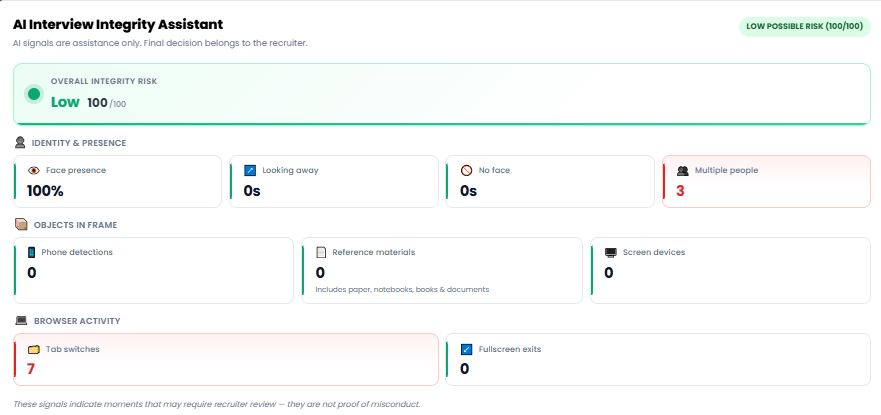
\includegraphics[width=0.9\textwidth,keepaspectratio]{../screenshoot/integrity.JPG}
  \caption{Exemple de rapport d'intégrité présenté au recruteur dans le tableau de bord NextHire.}
  \label{fig:integrity-report}
\end{figure}

\subsection{Écran de vérification pré-entretien}

Avant d'accéder à la salle d'entretien, le candidat passe par un écran de vérification
(composants \texttt{FaceVerification} et \texttt{VisionMonitor}). Celui-ci contrôle d'abord
les autorisations de la caméra et du microphone via l'API \textit{Permissions} du navigateur,
puis exécute un précontrôle en temps réel : présence et centrage du visage, qualité de
l'éclairage et unicité du visage dans le cadre. En parallèle, la vérification d'identité
faciale confronte l'image en direct à l'\textit{embedding} de référence du candidat
(InsightFace). Le candidat ne peut rejoindre l'entretien en direct que lorsque l'ensemble de
ces contrôles est validé (figure~\ref{fig:pre-interview}).

\begin{figure}[H]
  \centering
  \screenshot{pre-interview-verification.JPG}{Vérification caméra, micro et identité faciale}
  \caption{Écran de vérification pré-entretien.}
  \label{fig:pre-interview}
\end{figure}

\subsection{Vérification faciale \textit{fail-closed}}

Avant chaque entretien, un module de vérification d'identité compare l'image capturée en temps
réel par la webcam à la photo de profil enregistrée lors de l'enrôlement. La comparaison repose
sur un vecteur d'embedding de 512 dimensions calculé par InsightFace (modèle \texttt{buffalo\_l})
et une similarité cosinus. Le comportement est \textit{fail-closed} : toute condition anormale
bloque l'accès à la salle d'entretien plutôt que de le laisser passer.

\begin{itemize}
  \item \textbf{Service indisponible.} Si le micro-service de vérification faciale ne répond
        pas, la décision de démarrage est refusée (\texttt{status: 'failed',
        reason: 'face\_verification\_disabled'}).
  \item \textbf{Candidat non enrôlé.} Si aucun profil facial n'a été préalablement enregistré
        pour le candidat, l'accès est bloqué et un événement d'audit
        \texttt{NOT\_ENROLLED} est enregistré.
  \item \textbf{Similarité insuffisante.} Si la similarité cosinus entre les deux embeddings
        est inférieure au seuil $\tau = 0{,}60$, la vérification échoue et l'événement est journalisé
        avec les métadonnées d'audit (nombre de trames valides, score moyen).
\end{itemize}

La confidentialité est préservée par conception : les trames webcam transmises au serveur
pour la vérification ne sont jamais persistées et sont traitées en mémoire par le service
Python le temps du calcul de l'\textit{embedding}. Seul ce vecteur de 512 dimensions est
conservé, ce qui limite l'exposition des données biométriques au strict nécessaire. La figure~\ref{fig:face-verify-failed} illustre le cas où l'accès est refusé faute de correspondance d'identité.

\begin{figure}[H]
  \centering
  \screenshot{face-verify-failed.JPG}{Accès refusé : l'identité ne correspond pas au profil enrôlé}
  \caption{Comportement \textit{fail-closed} : accès à la salle refusé en cas de discordance d'identité.}
  \label{fig:face-verify-failed}
\end{figure}

\section{Tests}

\subsection{Test de la décision de vérification faciale}

Le module décisionnel de la vérification faciale est couvert par un test en
\texttt{node:assert} (\texttt{faceVerifyDecision.test.js}) regroupant 12~assertions. Celles-ci
vérifient le comportement \textit{fail-closed} de la décision de démarrage d'entretien :
la projection de sélection des candidats n'expose jamais l'\textit{embedding} facial parent,
une correspondance stricte n'est validée que lorsque le nombre minimal de trames concordantes
est atteint, et toute configuration ambiguë conduit à un refus plutôt qu'à une autorisation.

\section{Conclusion}

Ce sprint a fiabilisé la salle d'entretien en la dotant d'une surveillance d'intégrité multicouche et d'une vérification d'identité \textit{fail-closed}, sans jamais exposer les images brutes du candidat. Le sprint suivant complète la plateforme par l'aide à la décision (rapports pondérés, comparaison des candidats), le tableau de bord administrateur et la phase de finalisation.
          % Ch5 : Sprint 4 -- Consolidation
    \chapter[Sprint 5 : Aide à la décision et finalisation]{Sprint 5 : Aide à la décision, rapports pondérés\\et finalisation de la plateforme}
\begin{spacing}{1.2}
\minitoc
\thispagestyle{MyStyle}
\end{spacing}
\clearpage

\providecommand{\screenshot}[2]{%
  \IfFileExists{../screenshoot/#1}{%
    \includegraphics[width=0.9\textwidth,height=12cm,keepaspectratio]{../screenshoot/#1}%
  }{%
    \fbox{\parbox[c][4.5cm][c]{0.9\textwidth}{\centering\itshape
      Capture d'écran à insérer~: #2\\[4pt]
      \normalfont\small(fichier attendu~: \texttt{screenshoot/#1})}}%
  }%
}

\section{Introduction}

Le cinquième et dernier sprint enrichit la plateforme de ses fonctionnalités d'aide à la décision et la prépare au déploiement. Il introduit l'analyse multimodale post-entretien, la comparaison et le classement des candidats, le tableau de bord administrateur, puis consolide la sécurité et la conformité avant la phase de finalisation, de tests et de durcissement.

\section{Objectifs du sprint}

L'objectif principal de ce sprint est défini comme suit~:

\begin{quote}
\itshape Compléter NextHire par ses fonctionnalités d'aide à la décision, rapport d'entretien pondéré, analyse multimodale et comparaison des candidats, et finaliser la plateforme (tableau de bord administrateur, sécurité, conformité RGPD, tests et déploiement), la décision finale demeurant celle du recruteur.
\end{quote}

\subsection{Backlog du sprint}

Le tableau~\ref{tab:backlog-s5} présente le backlog du Sprint~5.

\begin{table}[H]
  \centering
  \footnotesize
  \renewcommand{\arraystretch}{1.3}
  \setlength{\tabcolsep}{5pt}
  \begin{tabularx}{\textwidth}{|>{\centering\arraybackslash}p{1.1cm}|>{\raggedright\arraybackslash}X|>{\centering\arraybackslash}p{1.8cm}|}
    \hline
    \rowcolor{blue!10}
    \textbf{ID} & \textbf{Récit utilisateur} & \textbf{Priorité} \\
    \hline
    S1 & En tant que recruteur, je veux un rapport d'entretien pondéré selon les critères du poste. & Haute \\
    \hline
    S2 & En tant que recruteur, je veux comparer et classer les candidats d'un même poste. & Haute \\
    \hline
    S3 & En tant que recruteur, je veux revoir en détail un entretien terminé (transcription, scores, intégrité). & Haute \\
    \hline
    S4 & En tant qu'administrateur, je veux superviser l'activité de la plateforme via un tableau de bord. & Moyenne \\
    \hline
    S5 & En tant qu'utilisateur, je veux que mes données soient protégées (RBAC, RGPD, chiffrement). & Haute \\
    \hline
  \end{tabularx}
  \caption{Backlog du Sprint~5 : Aide à la décision et finalisation.}
  \label{tab:backlog-s5}
\end{table}

\section{Concept de l'aide à la décision}

À l'issue des entretiens, NextHire assiste le recruteur dans sa décision sans jamais s'y substituer. Cette aide repose sur trois apports complémentaires~: un \textbf{rapport d'entretien pondéré}, produit par l'agent selon les critères du poste (compétences techniques, communication, expérience, comportement, intégrité)~; une \textbf{analyse multimodale} post-entretien, qui ajoute des indices affectifs (émotion faciale, sentiment vocal) à titre contextuel~; et un \textbf{classement multicritères} des candidats pour un même poste.

Conformément au principe de décision humaine retenu dès la conception, ces éléments \textit{informent} le recruteur~: aucune embauche n'est décidée automatiquement, et la décision finale reste une action explicite et tracée.

\section{Conception détaillée et architecture}

\subsection{Génération du rapport post-entretien}

La figure~\ref{fig:seq-report} illustre le flux de génération du rapport post-entretien,
déclenché automatiquement dès la fin de la session. Le rapport final combine l'évaluation
pondérée de l'agent IA, dont les poids sont configurés par offre via le Job Wizard et
somment à 100 (par exemple~: technique 40\,\%, communication 20\,\%, expérience 20\,\%,
comportement 10\,\%, intégrité 10\,\%), et l'analyse multimodale produite par le service
Analysis via un pipeline LangGraph.

\begin{sloppypar}
\begin{enumerate}
  \item \textbf{Déclenchement.} Dès que l'agent retourne \texttt{done:true}, le backend
        récupère le snapshot de la session (transcription, évaluations IRT, critères du
        poste) depuis MongoDB pour construire l'évaluation pondérée.

  \item \textbf{Analyse post-entretien.} Le backend déclenche le service Analysis en
        arrière-plan (fire-and-forget). Ce service exécute un pipeline LangGraph : il
        récupère le document complet de la session, appelle un LLM (fournisseur configurable~:
        Gemini, NVIDIA NIM, OpenAI, Anthropic ou Ollama local) pour analyser
        la transcription, évaluer les compétences et produire des recommandations, puis
        persiste la timeline comportementale dans MongoDB.

  \item \textbf{Construction du rapport recruteur.} Le backend assemble le rapport final
        à partir du snapshot de l'agent, du rapport d'intégrité et des résultats de
        l'analyse, le persiste dans MongoDB et notifie le client de la fin de la session.

  \item \textbf{Consultation.} Le recruteur ouvre la fiche depuis le tableau de bord. Le
        backend renvoie le rapport complet (scores, violations, transcription,
        recommandations de l'IA).
\end{enumerate}
\end{sloppypar}

\begin{figure}[H]
  \centering
  \resizebox{\textwidth}{!}{%
  \begin{tikzpicture}[
    font=\scriptsize,
    >={Stealth[length=2mm]},
    msg/.style={->, thin},
    ret/.style={->, thin, dashed},
    lbl/.style={font=\tiny, fill=white, inner sep=1pt, midway, above},
    lifeline/.style={dashed, thin, gray!70},
    phdr/.style={draw, fill=blue!12, rounded corners=2pt, align=center,
                 font=\scriptsize\bfseries, minimum height=0.65cm, minimum width=2.7cm},
  ]

  %% ── Participants ──────────────────────────────────────────────────────
  \node[phdr] at ( 0,  0) {React\\(Recruteur)};
  \node[phdr] at ( 4.5,0) {Node.js\\(:3001)};
  \node[phdr] at (10,  0) {Analysis Service\\(:8090)};
  \node[phdr] at (15.5,0) {LLM Provider\\(Gemini / NVIDIA / ...)};
  \node[phdr] at (21,  0) {MongoDB};

  %% ── Lifelines ─────────────────────────────────────────────────────────
  \draw[lifeline] ( 0,  -0.38) -- ( 0,  -14.5);
  \draw[lifeline] ( 4.5,-0.38) -- ( 4.5,-14.5);
  \draw[lifeline] (10,  -0.38) -- (10,  -14.5);
  \draw[lifeline] (15.5,-0.38) -- (15.5,-14.5);
  \draw[lifeline] (21,  -0.38) -- (21,  -14.5);

  %% ════════════════════════════════════════════════════════════════════════
  %% 1. Déclenchement
  %% ════════════════════════════════════════════════════════════════════════
  \node[font=\tiny\bfseries, anchor=east] at (-0.3,-0.75) {1.};
  \draw[->] (4.5,-0.75) -- ++(0.6,0) -- ++(0,-0.40) -- ++(-0.6,0);
  \node[font=\tiny, anchor=west] at (5.15,-0.95)
    {buildWeightedEvaluation(agentSnapshot, criteria)};
  \draw[msg] (4.5,-1.60) -- node[lbl] {findOne(callRoom) : transcript + integrityEvents} (21,-1.60);
  \draw[ret] (21,-2.20) -- node[lbl] {\{transcription, evaluations, violations\}} (4.5,-2.20);

  %% ════════════════════════════════════════════════════════════════════════
  %% 2. Analyse post-entretien
  %% ════════════════════════════════════════════════════════════════════════
  \node[font=\tiny\bfseries, anchor=east] at (-0.3,-2.85) {2.};
  \draw[msg] (4.5,-2.85) -- node[lbl] {POST /api/interviews/\{id\}/analyze-video} (10,-2.85);
  \draw[msg] (10,  -3.50) -- node[lbl] {findOne(callRoom) \{full document\}} (21,-3.50);
  \draw[ret] (21,  -4.10) -- node[lbl] {\{transcription, visionEvents, agentEvaluations\}} (10,-4.10);
  %% self-arrow: LangGraph pipeline
  \draw[->] (10,-4.70) -- ++(0.6,0) -- ++(0,-0.40) -- ++(-0.6,0);
  \node[font=\tiny, anchor=west] at (10.70,-4.90) {LangGraph pipeline (analyse multimodale)};
  \draw[msg] (10,  -5.60) -- node[lbl] {chat.completions(transcript + job\_context + criteria)} (15.5,-5.60);
  \draw[ret] (15.5,-6.20) -- node[lbl] {\{skills\_scores, strengths, gaps, recommendations\}} (10,-6.20);
  \draw[msg] (10,  -6.85) -- node[lbl] {PATCH callRoom \{behavioralTimeline, analyzed: true\}} (21,-6.85);
  \draw[ret] (10,  -7.45) -- node[lbl] {\{status: done\}} (4.5,-7.45);

  %% ════════════════════════════════════════════════════════════════════════
  %% 3. Construction du rapport recruteur
  %% ════════════════════════════════════════════════════════════════════════
  \node[font=\tiny\bfseries, anchor=east] at (-0.3,-8.10) {3.};
  \draw[->] (4.5,-8.10) -- ++(0.6,0) -- ++(0,-0.40) -- ++(-0.6,0);
  \node[font=\tiny, anchor=west] at (5.15,-8.30)
    {buildRecruiterReport(snapshot, integrity, analysis)};
  \draw[msg] (4.5,-9.00) -- node[lbl] {PATCH callRoom \{status:ended, recruiterReport, integrityReport\}} (21,-9.00);
  \draw[ret] (21, -9.60) -- node[lbl] {200 OK} (4.5,-9.60);
  \draw[ret] (4.5,-10.15) -- node[lbl] {emit("interview-ended", \{overallScore, reportReady: true\})} (0,-10.15);

  %% ════════════════════════════════════════════════════════════════════════
  %% 4. Consultation du rapport (recruteur)
  %% ════════════════════════════════════════════════════════════════════════
  \node[font=\tiny\bfseries, anchor=east] at (-0.3,-10.90) {4.};
  \draw[msg] ( 0,-10.90) -- node[lbl] {GET /api/callrooms/\{id\}} (4.5,-10.90);
  \draw[msg] (4.5,-11.55) -- node[lbl] {findOne(callRoom).populate(job, user)} (21,-11.55);
  \draw[ret] (21, -12.15) -- node[lbl] {\{recruiterReport, integrityReport, transcript, score\}} (4.5,-12.15);
  %% scoring breakdown note
  \draw[draw=orange!60, fill=orange!6, rounded corners=1pt, thin]
    (4.6,-12.70) rectangle (12.5,-13.35);
  \node[font=\tiny, anchor=west] at (4.7,-13.02)
    {tech 40\% · comm 20\% · exp 20\% · behav 10\% · integrity 10\%};
  \draw[ret] (4.5,-13.80) -- node[lbl] {200 OK \{fullReport, violations, ranking\}} (0,-13.80);

  \end{tikzpicture}%
  }
  \caption{Diagramme de séquence : génération du rapport post-entretien.}
  \label{fig:seq-report}
\end{figure}

\subsection{Analyse multimodale post-entretien}

Distincte du détecteur de fraude, dont les signaux restent de simples constats objectifs, l'analyse multimodale post-entretien enrichit l'évaluation du candidat par deux sources complémentaires de signal affectif. Pour l'\textbf{émotion faciale}, le service d'analyse s'appuie sur \textit{Py-Feat}, une boîte à outils entraînée sur le corpus \textit{AffectNet} d'images de visages réels. Plutôt que de prédire directement des probabilités d'émotion, souvent peu fiables, Py-Feat extrait les \textit{unités d'action faciales} (FACS, \textit{Facial Action Coding System}), mouvements élémentaires des muscles du visage, à partir desquelles sont dérivés les états émotionnels normalisés (joie, surprise, neutralité, etc.). Pour le \textbf{sentiment vocal}, la réponse du candidat, une fois transcrite par Faster-Whisper, est soumise à un modèle de classification de séquences fondé sur \textit{RoBERTa} (\texttt{cardiffnlp/twitter-roberta-base-sentiment-latest}), qui restitue une polarité (positif, neutre, négatif) assortie d'un score de confiance.

Il importe de souligner que ces signaux multimodaux sont traités comme des \textit{indices complémentaires}, destinés à contextualiser la prestation du candidat (par exemple, moduler le comportement de l'agent en cas de stress détecté), et non comme un déterminant de la décision. Aucune note d'embauche n'est calculée à partir de l'émotion ou du sentiment : l'évaluation des compétences repose sur le contenu des réponses, et la décision finale demeure une prérogative exclusive du recruteur humain. Ce parti pris répond aux préoccupations éthiques bien documentées concernant l'inférence d'états affectifs en contexte de recrutement.

\section{Réalisation et interfaces utilisateur}

\subsection{Rapport d'entretien pondéré}

Pour chaque entretien terminé, NextHire produit un rapport pondéré qui synthétise la performance du candidat selon les critères du poste, accompagné d'une recommandation d'embauche à quatre niveaux (\textit{Strong Hire}, \textit{Hire}, \textit{Maybe}, \textit{No Hire}). Le recruteur y retrouve les scores par critère, les points forts et les lacunes, ainsi que les indices comportementaux issus de l'analyse multimodale (figure~\ref{fig:report}).

\begin{figure}[H]
  \centering
  \screenshot{reporte.JPG}{Rapport d'entretien pondéré et recommandation d'embauche}
  \caption{Rapport d'entretien pondéré présenté au recruteur.}
  \label{fig:report}
\end{figure}

\subsection{Salles d'entretien et comparaison des candidats}

L'écran des salles d'entretien (route \texttt{/entreprise/:entrepriseId/interview-rooms},
composant \texttt{JobInterviewRooms}) permet au recruteur de créer une salle partageable
associée à un poste et de suivre les sessions des candidats. À l'issue de plusieurs entretiens,
l'écran de comparaison (\texttt{CandidateComparison}) classe les candidats selon un score
composite (technique, communication, résolution de problèmes, adéquation RH) et restitue le
résumé exécutif ainsi que la recommandation d'embauche produite par l'agent d'analyse
(figure~\ref{fig:candidate-comparison}).
Ce score composite de classement, score global, adéquation au poste, couverture des compétences, confiance du rapport et pénalité de biais, est distinct de la grille d'évaluation par question utilisée pendant l'entretien, qui repose sur le score adaptatif IRT-lite~$\theta$ mis à jour à chaque tour. Les deux grilles répondent à des objectifs complémentaires : l'une note la qualité de chaque réponse en temps réel, l'autre agrège les résultats de l'entretien pour permettre la comparaison entre candidats.

\begin{figure}[H]
  \centering
  \begin{subfigure}{0.6\textwidth}
    \centering
    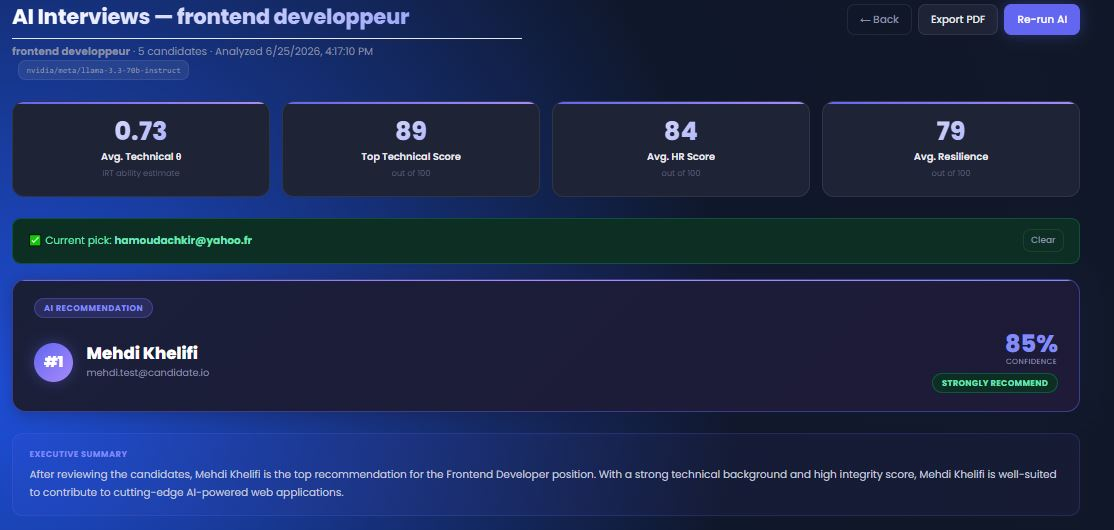
\includegraphics[width=\linewidth,keepaspectratio]{../screenshoot/compa1.JPG}
    \caption{Indicateurs agrégés et recommandation d'embauche de l'IA.}
    \label{fig:candidate-comparison-a}
  \end{subfigure}
  \par\medskip
  \begin{subfigure}{0.6\textwidth}
    \centering
    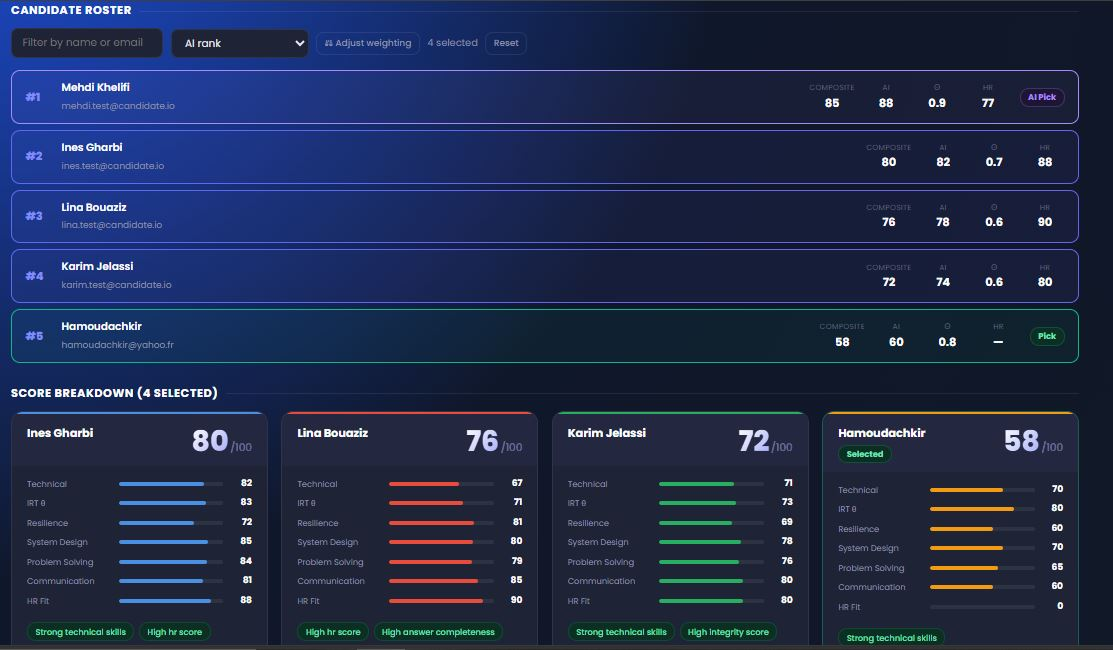
\includegraphics[width=\linewidth,keepaspectratio]{../screenshoot/compa2.JPG}
    \caption{Classement des candidats et détail des scores par dimension.}
    \label{fig:candidate-comparison-b}
  \end{subfigure}
  \par\medskip
  \begin{subfigure}{0.6\textwidth}
    \centering
    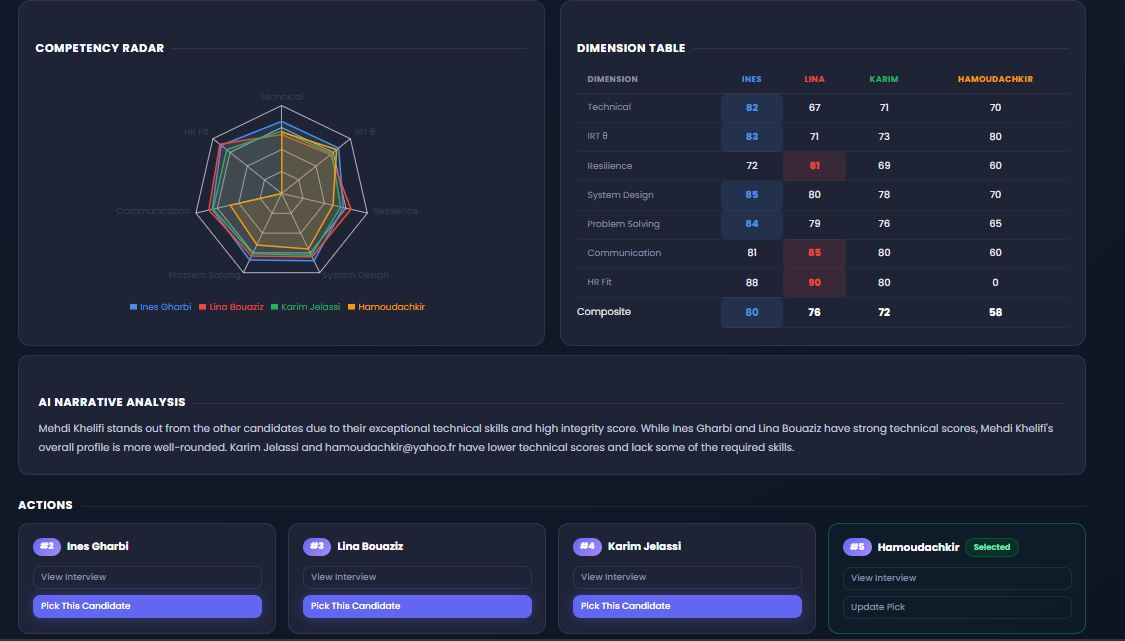
\includegraphics[width=\linewidth,keepaspectratio]{../screenshoot/compa3.JPG}
    \caption{Radar de compétences, tableau comparatif des dimensions et analyse narrative.}
    \label{fig:candidate-comparison-c}
  \end{subfigure}
  \caption{Écran de comparaison et de classement des candidats pour un poste.}
  \label{fig:candidate-comparison}
\end{figure}

\subsection{Écran de revue d'entretien}

L'écran de revue permet au recruteur d'examiner en détail un entretien terminé. Il affiche
en en-tête le nom du candidat, le poste concerné et la date de l'entretien. En dessous, une
transcription interactive liste chaque question posée par l'agent, la réponse du candidat,
le score et la justification produits par l'évaluation pondérée, ainsi que les éventuelles
violations détectées. Le rapport d'intégrité associé (niveau de risque, chronologie des
événements, recommandation) est présenté en regard, sans génération de fichier PDF externe
(figure~\ref{fig:interview-review}).

\begin{figure}[H]
  \centering
  \screenshot{interview-review.JPG}{Revue d'entretien : transcription, scores, intégrité}
  \caption{Écran de revue d'entretien côté recruteur.}
  \label{fig:interview-review}
\end{figure}

\subsection{Tableau de bord administrateur}

NextHire intègre un espace d'administration séparé, accessible sous le préfixe
\texttt{/dashboard}, protégé par un gardien de route dédié (\texttt{AdminProtectedRoute}).
Cet espace offre une vue centralisée de l'ensemble de la plateforme sans être lié à un
compte recruteur particulier.

\subsubsection{Vue d'ensemble et indicateurs clés}

La page d'accueil du tableau de bord agrège en temps réel les données de la plateforme via
l'endpoint \texttt{GET /api/admin/stats}. Six cartes d'indicateurs sont affichées en grille~:
le nombre de candidats inscrits, d'entreprises enregistrées, d'offres publiées, de
candidatures reçues, d'entretiens créés et d'entretiens planifiés. Deux graphiques complètent
cette vue~: un diagramme en anneau (\textit{donut chart}) représentant la répartition des
offres par statut, et un histogramme miniature indiquant l'évolution des candidatures dans
le temps. Un second diagramme en anneau distingue les entretiens confirmés des entretiens
en attente de planification (figure~\ref{fig:admin-dashboard}).

\begin{figure}[H]
  \centering
  \screenshot{admin-dashboard.JPG}{Tableau de bord admin : KPI, graphiques, listes récentes}
  \caption{Tableau de bord administrateur~: indicateurs en temps réel et graphiques d'activité.}
  \label{fig:admin-dashboard}
\end{figure}

\subsubsection{Gestion des entités}

La barre de navigation latérale donne accès à cinq sections de gestion~:

\begin{itemize}
  \item \textbf{Candidates} (\texttt{/dashboard/manage-candidates}) : liste paginée des
        candidats avec leurs informations de profil et leur statut de vérification.
  \item \textbf{Companies} (\texttt{/dashboard/manage-employees}) : gestion des comptes
        entreprise et de leurs informations administratives.
  \item \textbf{Jobs} (\texttt{/dashboard/jobs}) : consultation de toutes les offres publiées
        sur la plateforme, indépendamment de l'entreprise propriétaire.
  \item \textbf{Calendar} (\texttt{/dashboard/calendar}) : vue calendrier des entretiens
        planifiés sur l'ensemble des salles actives.
  \item \textbf{Settings} (\texttt{/dashboard/settings}) : paramètres globaux de la
        plateforme.
\end{itemize}

Cet espace d'administration permet de superviser l'activité de la plateforme et de
corriger d'éventuelles anomalies sans intervenir directement dans les comptes utilisateurs,
conformément au principe de séparation des responsabilités retenu lors de la conception.

\subsection{Messagerie et assistant conversationnel (NextBot)}

Au-delà du pipeline d'entretien, la page d'accueil intègre deux fonctionnalités
transverses visant à enrichir l'expérience candidat~: une messagerie directe avec le
recruteur et un assistant conversationnel alimenté par un LLM.

\subsubsection{Messagerie candidat--recruteur}

Les échanges sont persistés via un modèle \texttt{Message} (expéditeur, destinataire,
texte, horodatage, statut de lecture) exposé par une API REST dédiée
(\texttt{POST /api/messages/send}, \texttt{GET /api/messages/history/:user1/:user2},
\texttt{GET /api/messages/user/:userId}). La livraison en temps réel repose sur Socket.IO~:
l'émission d'un message déclenche un événement \texttt{send-message} côté serveur, relayé
au destinataire via \texttt{receive-message}, tandis que l'historique de la conversation est
chargé par requête REST à l'ouverture de la discussion. Le composant \texttt{MessagePopup}
fournit l'interface de discussion, réutilisée à la fois pour les échanges entre utilisateurs
et pour les interactions avec l'assistant.

\begin{figure}[H]
  \centering
  \screenshot{messaging.JPG}{Messagerie candidat--recruteur sur la page d'accueil}
  \caption{Interface de messagerie candidat--recruteur.}
  \label{fig:messaging}
\end{figure}

\subsubsection{NextBot : assistant conversationnel}

Le chatbot, nommé NextBot, est traité comme un utilisateur spécial (identifiant
\texttt{"bot"}) au sein de la même infrastructure de messagerie plutôt que comme un service
indépendant. Les requêtes adressées au bot (\texttt{POST /api/messages/bot/interaction})
sont transmises à l'API Groq (compatible OpenAI), via le modèle \texttt{gpt-oss-120b}. Pour
contextualiser ses réponses, le service enrichit le \textit{prompt} système avec le profil du
candidat (compétences, expérience) ainsi que les six derniers échanges de la conversation,
ce qui lui permet de fournir des conseils personnalisés sur la recherche d'emploi, la
préparation aux entretiens et la navigation sur la plateforme, sans recourir à une base
vectorielle~: il s'agit d'un enrichissement de contexte directement puisé dans MongoDB,
et non d'une recherche par similarité.

\begin{figure}[H]
  \centering
  \screenshot{chatbot.JPG}{Assistant conversationnel NextBot sur la page d'accueil}
  \caption{Assistant conversationnel NextBot.}
  \label{fig:chatbot}
\end{figure}

\section{Sécurité et conformité}

La sécurité de NextHire repose sur une stratégie de défense en profondeur : plusieurs couches
indépendantes couvrent l'identité, l'autorisation, la protection contre les abus, l'intégrité
de l'entretien et la conformité réglementaire. Cette section consolide l'ensemble des mécanismes
implémentés dans la plateforme.

\subsection{Autorisation par rôles -- RBAC}

Le contrôle d'accès basé sur les rôles est assuré par le middleware \texttt{requireEnterprise},
appliqué à tous les points de terminaison réservés aux recruteurs. Son comportement suit deux
chemins :

\begin{itemize}
  \item \textbf{Chemin rapide.} Si le JWT porte le champ \texttt{role = 'ENTERPRISE'},
        l'accès est accordé immédiatement sans requête base de données.
  \item \textbf{Repli base de données.} Pour les jetons antérieurs ne portant pas encore
        le champ \texttt{role} (compatibilité ascendante), le middleware interroge MongoDB
        (\texttt{User.findById().select('role').lean()}) et met à jour \texttt{req.user.role}
        en mémoire pour les middlewares aval.
\end{itemize}

Toute requête dont le rôle ne correspond pas à \texttt{ENTERPRISE} reçoit une réponse
\texttt{HTTP 403} avant d'atteindre la logique métier. Cette approche \textit{fail-closed}
garantit qu'une erreur de configuration (jeton sans rôle, base indisponible) bloque l'accès
plutôt que de l'autoriser par défaut.

\subsection{Limitation de débit}

Deux limiteurs de débit indépendants, fondés sur \texttt{express-rate-limit}, protègent les
points de terminaison à risque élevé, comme le récapitule le tableau~\ref{tab:rate-limiters}.

\begin{table}[H]
  \centering
  \footnotesize
  \renewcommand{\arraystretch}{1.3}
  \begin{tabularx}{\textwidth}{|>{\raggedright\arraybackslash}p{3.5cm}|>{\raggedright\arraybackslash}X|>{\raggedright\arraybackslash}p{2.8cm}|}
    \hline
    \textbf{Limiteur} & \textbf{Règle} & \textbf{Clé de comptage} \\
    \hline
    \texttt{aiGenerationRateLimiter} & 10 requêtes par minute par utilisateur (configurable via \texttt{AI\_GENERATION\_MAX\_PER\_MINUTE}) & \texttt{req.user.\_id} (repli sur IP) \\
    \hline
    \texttt{quizRateLimiter} & 3 soumissions par tranche de 24\,h par couple candidat\,+\,offre (configurable via \texttt{QUIZ\_MAX\_ATTEMPTS\_PER\_DAY}) & \texttt{candidateId-jobId} (repli sur IP) \\
    \hline
  \end{tabularx}
  \caption{Limiteurs de débit de la plateforme NextHire.}
  \label{tab:rate-limiters}
\end{table}

Les deux limiteurs partagent la même architecture de stockage : en développement, un compteur
en mémoire est utilisé ; en production, un stockage Redis (\texttt{rate-limit-redis}) est activé
par la variable d'environnement \texttt{QUIZ\_RATE\_LIMIT\_USE\_REDIS=true}. En cas d'échec de
connexion à Redis, le système se replie automatiquement sur le compteur en mémoire avec un
avertissement journalisé. Les requêtes ayant échoué à la validation (\textit{skipFailedRequests})
ne sont pas décomptées du quota.

\subsection{Conformité RGPD}

La plateforme a été conçue pour respecter les principes du Règlement Général sur la Protection
des Données :

\begin{itemize}
  \item \textbf{Consentement explicite.} Le candidat est informé, lors de l'enrôlement facial
        et avant le démarrage de l'entretien, que sa webcam et son microphone sont activés
        à des fins d'évaluation. L'entretien ne peut commencer sans validation de cette étape.
  \item \textbf{Minimisation des données biométriques.} Les trames webcam transmises au
        serveur pour la vérification faciale et la détection d'objets sont traitées en
        mémoire et ne sont jamais persistées~; seuls les embeddings (vecteurs de
        512 dimensions) qui en résultent sont conservés.
  \item \textbf{Décision finale humaine.} Le rapport post-entretien généré par l'IA fournit
        des scores, des points forts et des lacunes, et se conclut par une recommandation
        (\textit{Strong Hire / Hire / Maybe / No Hire}) ; la décision finale
        d'acceptation ou de refus reste une action explicite du recruteur, tracée en base de
        données. L'IA n'embauche pas : elle informe.
  \item \textbf{Chiffrement des données en transit.} Toutes les communications entre le
        navigateur et les services backend sont protégées par TLS (HTTPS). Les mots de
        passe ne sont jamais stockés en clair : seul leur condensé (\texttt{bcrypt} ou
        \texttt{bcryptjs} selon le module) est persisté.
\end{itemize}

\section{Tests et validation}

\subsection{Stratégie de tests et outillage}

La validation de NextHire suit le principe de la pyramide des tests : une base large de tests
unitaires rapides et isolés, un étage intermédiaire de tests d'intégration qui éprouvent les
frontières entre composants, et un sommet plus étroit de tests de bout en bout et de validation
système. Les dépendances lourdes (modèles PyTorch, Faster-Whisper, YOLO, accès réseau aux
API Groq et Edge TTS, MongoDB, Redis) sont remplacées par des doublures
(\textit{stubs} enregistrés dans \texttt{sys.modules} côté Python, données factices côté
Node.js), de sorte que la suite s'exécute en quelques secondes, sans GPU ni clé d'API. Les
tests qui exigent une infrastructure réelle sont isolés et ignorés automatiquement lorsque
celle-ci est absente. Le tableau~\ref{tab:test-frameworks} récapitule les frameworks employés
par service et par niveau.

\begin{table}[H]
  \centering
  \footnotesize
  \renewcommand{\arraystretch}{1.3}
  \setlength{\tabcolsep}{5pt}
  \begin{tabularx}{\textwidth}{|>{\raggedright\arraybackslash}p{3.4cm}|>{\raggedright\arraybackslash}p{2.3cm}|>{\raggedright\arraybackslash}p{3.0cm}|>{\raggedright\arraybackslash}X|}
    \hline
    \rowcolor{blue!10}
    \textbf{Service} & \textbf{Niveau} & \textbf{Framework} & \textbf{Fichier représentatif} \\
    \hline
    Backend Node.js & Unitaire & \texttt{node:assert} & \texttt{faceVerifyDecision.test.js} \\
    \hline
    Moteur d'entretien (\texttt{voice\_engine}) & Unitaire & \texttt{unittest} + stubs & \texttt{test\_interview\_agent\_conversation.py} \\
    \hline
    Service d'analyse (\texttt{analysis\_service}) & Unitaire / intégration & \texttt{pytest} & \texttt{test\_report\_schema.py} \\
    \hline
    Frontend (React) & Bout en bout & Playwright & \texttt{e2e-rh-job-match.spec.js} \\
    \hline
    Système & Validation & Scripts Python & \texttt{tests/} (charge, chaos, ML, intégrité) \\
    \hline
  \end{tabularx}
  \caption{Frameworks de test par service et par niveau.}
  \label{tab:test-frameworks}
\end{table}

\subsection{Tests unitaires du service d'analyse}

Le service d'analyse post-entretien constitue la suite la plus fournie : neuf modules de tests
\texttt{pytest} sous \texttt{analysis\_service/tests/}. Ils couvrent la validation du schéma de
rapport (\texttt{report\_schema}), la fusion et le polissage des rapports, l'extraction des
métadonnées d'entretien, le service FFmpeg et le service média. Le tableau~\ref{tab:analysis-tests}
détaille la répartition et les résultats d'exécution.

\begin{table}[H]
  \centering
  \footnotesize
  \renewcommand{\arraystretch}{1.25}
  \setlength{\tabcolsep}{6pt}
  \begin{tabularx}{\textwidth}{|>{\raggedright\arraybackslash}X|>{\centering\arraybackslash}p{2.0cm}|>{\centering\arraybackslash}p{2.0cm}|}
    \hline
    \rowcolor{blue!10}
    \textbf{Module de test} & \textbf{Tests} & \textbf{Réussis} \\
    \hline
    \texttt{test\_enhanced\_report.py} & 48 & 48 \\ \hline
    \texttt{test\_media\_service.py} & 33 & 33 \\ \hline
    \texttt{test\_report\_polish\_merge.py} & 22 & 22 \\ \hline
    \texttt{test\_ffmpeg\_service.py} & 19 & 19 \\ \hline
    \texttt{test\_interview\_metadata.py} & 19 & 19 \\ \hline
    \texttt{test\_phase2\_features.py} & 18 & 17 (1 ignoré) \\ \hline
    \texttt{test\_report\_schema.py} & 15 & 15 \\ \hline
    \texttt{test\_report\_quality.py} & 9 & 9 \\ \hline
    \texttt{test\_report\_new\_fields.py} & 8 & 8 \\ \hline
    \rowcolor{gray!8}
    \textbf{Total} & \textbf{191} & \textbf{190 (1 ignoré)} \\ \hline
  \end{tabularx}
  \caption{Résultats d'exécution des tests unitaires du service d'analyse.}
  \label{tab:analysis-tests}
\end{table}

\subsection{Tests d'intégration, de bout en bout et de validation système}

\paragraph{Bout en bout (Frontend).} Un scénario Playwright
(\texttt{e2e-rh-job-match.spec.js}) pilote un navigateur réel pour valider le parcours
recruteur d'appariement candidat~/~offre (\textit{job match}) à travers l'application et le
backend. Ce test nécessite la pile complète en cours d'exécution et est donc exécuté lors des
campagnes d'intégration.

\paragraph{Validation système (suite Phase~6).} Le répertoire \texttt{tests/} à la racine
regroupe une suite de validation système couvrant plusieurs préoccupations transversales :
tests de charge (\texttt{load/} : \textit{locust}, exécution concurrente d'entretiens, charge
WebSocket), tests de robustesse (\texttt{chaos/} : pannes simulées de MongoDB, de Redis, du
\textit{worker} et expiration GPU), validation ML (\texttt{ml/} : détection de dérive et
validation en mode ombre), intégrité des rapports (\texttt{integrity/}) et audit de cohérence
(\texttt{audit/} : détection d'orphelins, rejeu déterministe). Ces tests s'exécutent contre une
infrastructure vivante et sont déclenchés manuellement lors des campagnes de validation.

\subsection{Synthèse cumulative}

Le tableau~\ref{tab:cumulative-tests} consolide le décompte et les taux de réussite des tests
automatisés exécutés sans infrastructure externe. L'ensemble des 199~tests unitaires
(\texttt{pytest} et \texttt{unittest}) ainsi que les 12~assertions du test Node.js réussissent,
soit un taux de réussite de 100~\%. Chaque dépendance native lourde est interceptée avant import,
ce qui permet à la suite de s'exécuter en quelques secondes.

\begin{table}[H]
  \centering
  \footnotesize
  \renewcommand{\arraystretch}{1.25}
  \setlength{\tabcolsep}{6pt}
  \begin{tabularx}{\textwidth}{|>{\raggedright\arraybackslash}X|>{\centering\arraybackslash}p{1.8cm}|>{\centering\arraybackslash}p{1.8cm}|>{\centering\arraybackslash}p{2.0cm}|}
    \hline
    \rowcolor{blue!10}
    \textbf{Service} & \textbf{Fichiers} & \textbf{Tests} & \textbf{Taux de réussite} \\
    \hline
    \texttt{analysis\_service} (pytest) & 9 & 190 & 100~\% \\ \hline
    \texttt{voice\_engine} (unittest) & 2 & 9 & 100~\% \\ \hline
    Backend Node.js (\texttt{node:assert}) & 1 & 12 assertions & 100~\% \\ \hline
    Frontend (Playwright, E2E) & 1 & 2 scénarios & infrastructure requise \\ \hline
    \rowcolor{gray!8}
    \textbf{Total (hors infrastructure)} & \textbf{12} & \textbf{211 vérifications} & \textbf{100~\%} \\ \hline
  \end{tabularx}
  \caption{Synthèse cumulative des tests automatisés de NextHire.}
  \label{tab:cumulative-tests}
\end{table}

\subsection{Couverture de code}

La couverture du service d'analyse a été mesurée avec \texttt{pytest-cov}. Sur l'ensemble du
paquet \texttt{app} (4218~instructions), la suite couvre 45~\% des instructions. Cette valeur
globale reflète un choix de périmètre délibéré : les tests ciblent en priorité le cœur métier
(schéma et construction des rapports, évaluation des questions, appariement aux offres,
services média), tandis que les couches d'infrastructure (workers RQ, registre de modèles ML
multi-locataires, RBAC, métriques) sont éprouvées au niveau de l'intégration système. Le
tableau~\ref{tab:analysis-coverage} présente la couverture des modules les plus exercés.

\begin{table}[H]
  \centering
  \footnotesize
  \renewcommand{\arraystretch}{1.25}
  \setlength{\tabcolsep}{6pt}
  \begin{tabularx}{\textwidth}{|>{\raggedright\arraybackslash}X|>{\centering\arraybackslash}p{2.6cm}|}
    \hline
    \rowcolor{blue!10}
    \textbf{Module} & \textbf{Couverture (instructions)} \\
    \hline
    \texttt{schemas/report\_schema.py} & 99~\% \\ \hline
    \texttt{services/report\_service.py} & 91~\% \\ \hline
    \texttt{services/question\_evaluator.py} & 89~\% \\ \hline
    \texttt{services/sentiment\_service.py} & 86~\% \\ \hline
    \texttt{services/job\_match\_service.py} & 84~\% \\ \hline
    \texttt{services/ffmpeg\_service.py} & 81~\% \\ \hline
    \texttt{services/qna\_service.py} & 79~\% \\ \hline
    \texttt{services/interview\_metadata.py} & 54~\% \\ \hline
    \rowcolor{gray!8}
    \textbf{Ensemble du paquet \texttt{app}} & \textbf{45~\%} \\ \hline
  \end{tabularx}
  \caption{Couverture d'instructions par module du service d'analyse (\texttt{pytest-cov}).}
  \label{tab:analysis-coverage}
\end{table}

\section{Conclusion}

Ce dernier sprint a complété NextHire par ses fonctionnalités d'aide à la décision, analyse multimodale, comparaison et classement des candidats, revue d'entretien, et par son tableau de bord administrateur, tout en renforçant la sécurité et la conformité RGPD. La suite de tests automatisés (211~vérifications, taux de réussite de 100~\% hors infrastructure) et les mesures de performance valident la faisabilité technique de la solution. La conclusion générale du rapport reviendra sur les apports de la plateforme et ses perspectives d'évolution.
          % Ch6 : Sprint 5 -- Finalisation
    
    % Conclusion du rapport
    \chapter*{CONCLUSION ET PERSPECTIVES}
\markboth{\MakeUppercase{CONCLUSION GÉNÉRALE}}{}
\addcontentsline{toc}{chapter}{CONCLUSION GÉNÉRALE}
\adjustmtc
\thispagestyle{MyStyle}

% Guide pour la rédaction de la Conclusion et Perspectives

La \textbf{Conclusion Générale} a pour objectif de résumer les contributions du projet et d’ouvrir des perspectives d’évolution. Elle doit inclure les éléments suivants :

\begin{itemize}
    \item \textbf{Synthèse des réalisations :} Récapitulez les principales étapes du projet et les résultats obtenus.
    \item \textbf{Impact et apports :} Mettez en avant l'importance du projet et les bénéfices qu’il apporte aux utilisateurs ou à l’entreprise.
    \item \textbf{Limites :} Identifiez brièvement les contraintes ou améliorations possibles.
    \item \textbf{Perspectives d’évolution :} Décrivez les pistes d’amélioration et d’extension du projet :
    \begin{itemize}
        \item \textbf{À court terme :} Actions immédiates après la mise en place du projet.
        \item \textbf{À moyen terme :} Évolutions possibles dans les mois ou années à venir.
        \item \textbf{À long terme :} Vision future et extensions potentielles du projet.
    \end{itemize}
\end{itemize}

\noindent Cette conclusion doit être rédigée de manière synthétique et mettre en avant la valeur ajoutée du projet ainsi que son potentiel d’évolution.


    % Bibliographie
    \addcontentsline{toc}{chapter}{WEBOGRAPHIE}

\adjustmtc
\renewcommand\bibname{WEBOGRAPHIE}

\begin{thebibliography}{9}

\bibitem{TALAN}
\textbf{Talan Tunisie}. Page web de l'entreprise \textbf{[en ligne]}.\\Dernière consultation : 21/03/2025.\\Disponible à : \url{https://www.talan.com/global/fr}


\end{thebibliography}


    % Dernière page (A4 plein format) — pas de page blanche traînante après la 4e de couverture
    \clearpage
    \pagestyle{empty}
    \includepdf[pages=1, width=\paperwidth, height=\paperheight, pagecommand={\thispagestyle{empty}}]{end.pdf}

\end{document}
